% Monografia para Projeto de Fim de Curso - Exemplo no LaTeX
%-----------------------------------------------------------


%---------------Inicialização de pacotes--------------------

\documentclass[12pt,a4paper,notitlepage,twoside]{book}

\usepackage{graphicx}
\usepackage[utf8]{inputenc}
\usepackage[brazil]{babel}		
\usepackage[T1]{fontenc}
\usepackage{amsmath,amssymb}
\usepackage{amsthm,amsfonts}
\usepackage{bm}
\usepackage[short]{optidef}
\usepackage[table]{xcolor}
\definecolor{lightgray}{gray}{0.9}

\usepackage[hidelinks]{hyperref}

\usepackage{abntex2abrev}
%\usepackage[num, overcite, abnt-emphasize=bf, abnt-etal-list=3]{abntex2cite} 
\usepackage[num, abnt-emphasize=bf, abnt-etal-list=3]{abntex2cite} 
\citebrackets[]

\usepackage{setspace}
\usepackage{parskip}
\usepackage[toc,page]{appendix}
\usepackage[framed, numbered]{matlab-prettifier}

\usepackage{import}
\usepackage{booktabs}
\usepackage{float}
\usepackage[skip=10pt]{caption}

\usepackage[a4paper,top=30mm,bottom=30mm,inner=30mm,outer=25mm,headheight=7mm,headsep=6mm,footskip=7mm]{geometry}
\usepackage{enumerate}


\usepackage{tikz}
\usetikzlibrary{trees}
\usepackage[american]{circuitikz}
\usepackage{pgfplots}
\pgfplotsset{compat=1.16}
\usepackage{tikz-qtree}

\makeindex

\setstretch{1.10} %%um pouco melhor que espaçamento simples

\renewcommand{\lstlistingname}{Código}
\renewcommand{\lstlistlistingname}{Lista de Códigos}
\lstset{%
        inputencoding=utf8,
        extendedchars=true,
        literate=%
        {é}{{\'{e}}}1
        {è}{{\`{e}}}1
        {ê}{{\^{e}}}1
        {ë}{{\¨{e}}}1
        {É}{{\'{E}}}1
        {Ê}{{\^{E}}}1
        {û}{{\^{u}}}1
        {ù}{{\`{u}}}1
        {ú}{{\'{u}}}1
        {â}{{\^{a}}}1
        {à}{{\`{a}}}1
        {á}{{\'{a}}}1
        {ã}{{\~{a}}}1
        {Á}{{\'{A}}}1
        {Â}{{\^{A}}}1
        {Ã}{{\~{A}}}1
        {ç}{{\c{c}}}1
        {Ç}{{\c{C}}}1
        {õ}{{\~{o}}}1
        {ó}{{\'{o}}}1
        {ô}{{\^{o}}}1
        {Õ}{{\~{O}}}1
        {Ó}{{\'{O}}}1
        {Ô}{{\^{O}}}1
        {î}{{\^{i}}}1
        {Î}{{\^{I}}}1
        {í}{{\'{i}}}1
        {Í}{{\~{Í}}}1
}
\usepackage{longtable}

%---------------Início do documento-------------------------

\begin{document}


\begin{titlepage}
\begin{center}
{\large Universidade Federal de Minas Gerais\\
Escola de Engenharia \\
Curso de Graduação em Engenharia de Controle e Automação\\}

\vspace{6cm}
{\bf\Large Controle Ótimo Aplicado em\vspace{0.2cm}

um Veiculo Elétrico de Competição}
\vspace{4cm}

%\hspace{0.3\textwidth} \parbox{0.65\textwidth}
{\large Michael Feliphe da Silva Barbosa}
\vspace{2cm}  
   
\vspace{2cm}          
%\hspace{0.3\textwidth} 
{\large Orientador: Prof. Dimas Abreu Archanjo Dutra, Dr.}\\
{\large Supervisor: Prof. Víctor Costa da Silva Campos, Dr.}

\vfill
%\hspace{0.3\textwidth} 
{\large Belo Horizonte, Julho de 2020 }
\end{center}

\end{titlepage}

\newpage
\clearpage
\thispagestyle{empty}


\begin{titlepage}

\centering
\textbf{Monografia}\\
\vspace{2cm}
\centering
\textbf{Título da Monografia}\\
\vspace{5cm} 

\parbox{1.0\textwidth} 
{\large 
Monografia submetida à banca examinadora
designada pelo Colegiado Didático do Curso de
Graduação em Engenharia de Controle e
Automação da Universidade Federal de Minas
Gerais, como parte dos requisitos para aprovação na
disciplina Projeto Final de Curso II.}

\vspace{7cm} 
\centering
Belo Horizonte, Julho de 2014

\end{titlepage}


\pagenumbering{roman}
\addcontentsline{toc}{chapter}{Resumo}

\begin{center}
\huge{{\bf Resumo}}
\vspace{2cm}
\end{center}

No Resumo, em uma única página, em no máximo dois parágrafos, você explicita os seguintes itens: objetivos do projeto e descrição sucinta do local onde ele foi desenvolvido; metodologia utilizada; e resultados alcançados. Leitores experientes decidem se prosseguirão para a leitura do texto completo após lerem o resumo, a conclusão e a introdução. Por isso nestes lugares você deve colocar um esforço maior de convencimento. Além disso, a linguagem utilizada deve ser acessível a leitores com pouca familiaridade com a área, limitando o uso de jargões.
 
\begin{sloppypar}
Este novo parágrafo serve para mostrar que ao pular uma ou mais linhas no texto do arquivo .tex, o \TeX\ entende que você está iniciando outro parágrafo. O comando sloppypar força o texto a não ultrapassar as margens. Só deve ser usado se este problema ocorrer.
\end{sloppypar}

 
\clearpage
\thispagestyle{empty}
\cleardoublepage


\addcontentsline{toc}{chapter}{Abstract}

\begin{center}
\huge{{\bf Abstract}}
\vspace{2cm}
\end{center}

The UFMG's electric vehicle, the DT1, is a prototype used in energy efficiency competitions. 
Its most recent autonomy measurement is a $226.9$ [km/kWh] mark held in the 2019 Shell EcoMarathon Americas student competition. 
This end-of-course project aims to determine, based on the application of the optimal control theory, the sequence and activation of the electric motor 
(track strategy) so that the autonomy of the DT1 is the maximum possible on the current track of the Shell EcoMarathon Americas competition at the Sonoma raceway.

To achieve this objective, a mathematical model of the longitudinal dynamics of the prototype vehicle was first determined. 
Based on this model and the determinations of the Shell EcoMarathon organization for measuring autonomy, an optimal control problem was formulated that 
was solved using the FALCON.m software. However, the vehicle model has not been validated experimentally, due to the realization of this project during 
the Emergency Remote Education regime and this does not allow us to state that the track strategy found is optimal for the real case.

\textbf{Keywords} -- Electric Vehicle, Energy Efficiency, Shell EcoMarathon Competition, Vehicle Model, Optimal Control Problem, FALCON.m.

 
\clearpage
\thispagestyle{empty}
\cleardoublepage


\addcontentsline{toc}{chapter}{Agradecimentos}

\begin{center}
\huge{{\bf Agradecimentos}}
\vspace{4cm}
\end{center}

Aqui vai o texto dos agradecimentos.
 
\clearpage
\thispagestyle{empty}
\cleardoublepage
\tableofcontents
%\markboth{Conteúdo}{Conteúdo}

\clearpage
%\thispagestyle{empty}
%\cleardoublepage

% Normalmente, este arquivo só contém isto.
\listoffigures
\addcontentsline{toc}{chapter}{Lista de Figuras}
%\markboth{Lista de Figuras}{Lista de Figuras}

\clearpage
%\thispagestyle{empty}
%\cleardoublepage

% Normalmente, este arquivo só contém isto.
\listoftables
\addcontentsline{toc}{chapter}{Lista de Tabelas}
%\markboth{Lista de Tabelas}{Lista de Tabelas}

\clearpage
%\thispagestyle{empty}
%\cleardoublepage

% Normalmente, este arquivo só contém isto.

\pagenumbering{arabic}
\setcounter{page}{1}
\chapter{Introdução}
\label{chap:intro}
\thispagestyle{empty}

Esté capitulo explica a motivação e objetivos deste projeto de otimização do desempenho em competições de um veículo elétrico protótipo de alta eficiência.
Apresenta a equipe de competição estudantil Milhagem UFMG onde este PFC foi realizado. E, também, descreve a estrutura desta monografia.

\section{Motivação e Justificativa}
\label{sec:motivacao}

A equipe Milhagem UFMG constrói protótipos de veículos para participar de competições
de eficiência energética. Atualmente a equipe possui dois veículos: o M84 equipado com um motor a combustão interna a gasolina e o DT1,
 apresentado na Figura \ref{fig:DT1}, que possui motor elétrico e bateria. As competições em que a
equipe participa são a Shell Eco-Marathon Brasil (nacional) e a Shell EcoMarathon Americas (internacional).
Nestas competições os veículos devem consumir a
menor quantidade de energia para percorrer trajeto, ou seja, devem ter a maior eficiência
energética.

\begin{figure}[h]
    \centering
    \caption{Veículo elétrico protótipo DT1}
    \label{fig:DT1}
    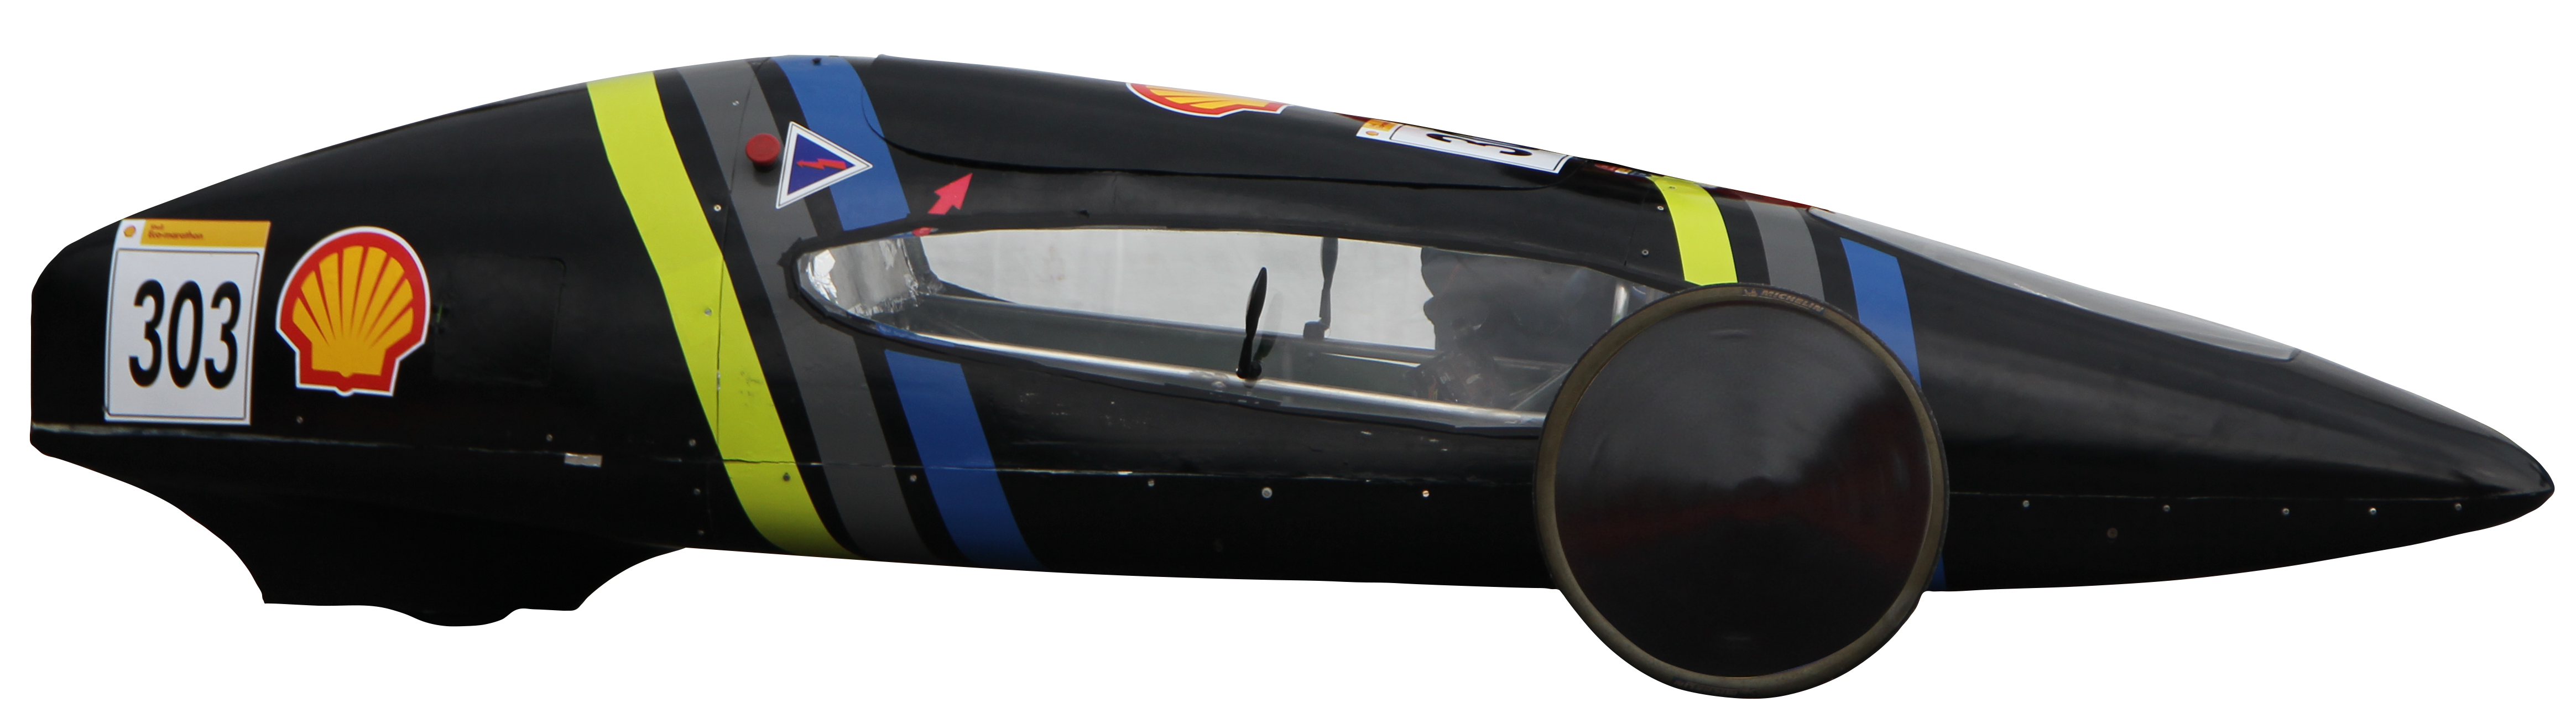
\includegraphics[scale=0.11]{Introducao/Figuras/dt1.png}
    \caption*{\footnotesize{Fonte: Equipe Milhagem UFMG}}
\end{figure}

Os principais fatores que influenciam no consumo de energia do veículo são a
aerodinâmica, o peso total, a resistência ao rolamento, o relevo do trajeto e a estratégia
de pista. Essa estratégia consiste na forma e nos momentos em que o motor deve ser
acionado. Um exemplo de uma estratégia de pista muito utilizada nesses protótipos é a
estratégia start-stop, na qual o motor é desligado quando a velocidade é maior que 30
km/h e religado apenas quando é menor que 20 km/h, semelhante a um controle on-off
com histerese.

Durante a avaliação da eficiência energética de um protótipo ele deve seguir as seguintes
restrições: posições inicial e final fixas, velocidade inicial nula, velocidade instantânea
máxima e velocidade média mínima. Uma vez que essas restrições permitem inúmeras
estratégias de pista tem-se a necessidade encontrar a estratégia que maximize a
eficiência energética do veículo durante a avaliação de consumo.

% A teorias de controle ótimo fornece o embasamento para a
% que a estratégia de maior eficiência seja calculada numericamente. Para isso antes é necessário
%  a determinação do modelo matemático que represente o comportamento dinâmico do veiculo.

\section{Objetivos do Projeto}
\label{sec:objetivos}

Tendo em vista o exposto acima, este projeto tem por objetivos direcionados ao protótipo DT1:

\begin{enumerate}[(a)]
    \item Definir o modelo matemático para a dinâmica do protótipo;
    \item Formular o problema de controle ótimo (OCP) pra obter a estratégia ótima;
    \item Implementar o algoritmo para solução desse OCP;
    \item Definir a estratégia ótima para a pista da Shell EcoMarathon Américas de 2019.
\end{enumerate}

\section{Local de Realização}
\label{sec:empresa}


Esse projeto foi desenvolvido na equipe de de competição Milhagem UFMG, na qual o autor foi integrante de 2013 à 2015 e em 2018. A equipe é composta por alunos de graduação em engenharia de diversos períodos e sua sede é no Departamento de Engenharia Mecânica da UFM.
Foi fundada, sobre orientação do
professor Paulo Iscold, em 2005 no Centro de Estudos Aeronáuticos (CEA) do qual fez
parte até 2006.
De 2006 a 2011 o projeto da equipe ficou suspenso retornando as atividades, sobre orientação do professor Fabrício Pujatti, no Centro de Tecnologia
de Mobilidade (CTM). A equipe ja desenvolveu 6 veículos, sendo DT1 o primeiro elétrico, e participou de de 10 competições com os seguintes resultados:


\begin{itemize}
    \item Maratona Universitária de Eficiência Energética
          \begin{itemize}
              \item  Categoria gasolina
                    \begin{itemize}
                        \item 2005: 2º Lugar, com a marca de $227,6$ [km/L]
                        \item 2006: 1º Lugar, com a marca de $598,9$ [km/L]
                        \item 2011: 5º Lugar, com a marca de $199,0$ [km/L]
                        \item 2013: 4º Lugar, com a marca de $234,9$ [km/L]
                    \end{itemize}
          \end{itemize}
    \item Shell Eco-marathon Brasil
          \begin{itemize}
              \item  Categoria gasolina
                    \begin{itemize}
                        \item 2016: 2º Lugar, com a marca de $196,0$ [km/L]
                    \end{itemize}
              \item  Categoria elétrico
                    \begin{itemize}
                        \item 2017: 3º Lugar, com a marca de $315,6$ [km/kWh]
                        \item 2018: 1º Lugar, com a marca de $266,4$ [km/kWh]
                    \end{itemize}
          \end{itemize}
    \item Shell Eco-marathon Americas
          \begin{itemize}
              \item  Categoria elétrico
                    \begin{itemize}
                        \item 2018: 6º Lugar, com a marca de $266,5$ [km/kWh]
                        \item 2019: 2º Lugar, com a marca de $226,9$ [km/kWh]
                    \end{itemize}
          \end{itemize}
\end{itemize}

\section{Estrutura da Monografia}
\label{sec:organizacao}

O relatório está dividido em cinco capítulos. Este capítulo apresentou uma introdução ao projeto a ser descrito nos capítulos seguintes. 
O Capítulo \ref{chap:revisao} é uma revisão bibliográfica que dos princípios básicos de modelagem veicular e controle ótimo de forma que abrange todos os
conceitos necessários para um melhor entendimento do projeto. O Capítulo \ref{chap:metodologia} aborda a metodologia de desenvolvimento do modelo matemático do DT1 e de implementação implementação do software
para otimização da estrategia de pista. Os resultados obtidos no projeto são apresentados no Capítulo \ref{chap:resultados} e no 
Capitulo \ref{chap:conclusao} tem-se a conclusão da monografia com algumas sugestões para trabalhos futuros e dificuldades encontradas durante a realização do projeto.

\clearpage
\chapter[Revisão Bibliográfica]{Revisão Bibliográfica}
\label{chap:revisao_bibliografica}
\thispagestyle{empty}

Este capitulo é divido em duas seções que visam apresentar os conceitos necessários para a compreensão deste PFC.
Na primeira seção são aprensados conceitos para uma modelagem matemática da dinâmica de um veiculo em baixas velocidades.
São apresentado na segunda seção uma introdução à teoria de controle ótimo e a utilização de programação não linear na solução
de problemas de controle ótimo.

\section{Modelo do veículo}
\label{sec:modelo}

Um modelo matemático, ou apenas modelo, é um conjunto de equações que descreve de forma adequada o comportamento de um sistema que deseja-se estudar.
Uma forma usual de classificação dos métodos de modelagem é separa-los nas categorias: modelagem caixa branca, modelagem caixa preta e modelagem
caixa cinza.
A modelagem caixa branca, também conhecida como modelagem conceitual, consiste na aplicação princípios fundamentais e por isso exige um conhecimento
da natureza do sistema.
A modelagem caixa preta, ou modelagem empírica, é baseada na aplicação de técnicas de identificação de sistemas que exigem pouco ou
nenhum conhecimento do sistema.
Já na modelagem caixa cinza sáo utilizadas técnicas que estão entre a modelagem caixa branca e a modelagem caixa preta\cite{book:Aguirre}.

Nessa seção o método de modelagem aplicado é de modelagem caixa branca. A partir da aplicação da segunda lei de Newton no
veiculo representado no diagrama da Figura \ref{fig:diag_forcas_veiculo}, obtém-se a equação que descreve a dinâmica longitudinal do mesmo

\begin{equation}
	\label{eq:SomaForcas}
	m \cdot \dot v	= F_t - (F_a +	F_g + F_p)
	\enspace,
\end{equation}

em que $m$ é a massa total, $v$ é a velocidade, $F_{t}$ é a propulsão feita pelo motor subtraída as perdas do sistema de transmissão, $F_{a}$ é o
arrasto aerodinâmico, $F_g$ é a componente do peso que esta direção da velocidade e $F_{p}$ é a resistência ao rolamentos dos pneus no pista.
Os modelos que descrevem a forças $F_{a}$, $F_g$, $F_{p}$ e $F_{t}$ estão apresentados nas subseções a seguir.

\begin{figure}[H]
	\centering
	\caption{Diagrama de forças de um veículo em movimento}
	\label{fig:diag_forcas_veiculo}
	\begin{normalsize}
		\import{DescricaoProcesso/Figuras/}{diagrama_forcas_veiculo.pdf_tex}
	\end{normalsize}
	\caption*{\footnotesize Fonte: Elaborado pelo autor.}
\end{figure}

\subsection{Arrasto Aerodinâmico}
\label{subsec:arrasto_aerodinamico}

O movimento de um objeto imerso em um fluido sofre uma resistência causada por esse fluido. No
caso de veículos que se deslocando no ar, essa
resistência é chamada de arrasto aerodinâmico.
Pode-se aproximar o calculo dessa força $F_{a}$ com a equação

\begin{equation}
	\label{eq:Fa}
	F_a(v) = \frac{\rho \cdot a_f \cdot c_d \cdot v^2}{2}
	\enspace,
\end{equation}

em que $v$ é a velocidade do veiculo em relação ao vento, $\rho$ a densidade do ar, $a_{f}$ a área frontal do
veiculo e $c_{d}$ o coeficiente de arrasto aerodinâmico.
O coeficiente $c_{d}$ é um numero adimensional e depende da geometria veiculo, é determinado por meio de simulações em \textit{software} de fluido
dinâmica
computacional (CFD, do inglês \textit{computational fluid dynamics}) e/ou experimentos em túnel de vento\cite{book:guzzella2012vehicle}. Alguns
valores típicos de $C_{d}$ para diferentes tipos de
veículos são apresentados na Tabela \ref{tab:ComparacaoCD}.

\begin{table}[H]
	\centering
	\caption{Comparação do $c_{d}$ de diferentes tipos veículos}
	\rowcolors{1}{}{lightgray}
	\begin{tabular}{ll}
		\toprule
		\textbf{Veiculo} & \boldsymbol{$c_{d}$} \\
		\hline
		Carro            & 0,3 - 0,4            \\
		Ônibus           & 0,6 - 0,7            \\
		Caminhão         & 0,6 - 1,0            \\
		Moto             & 0,5 - 1,0            \\
		\bottomrule
	\end{tabular}
	\caption*{\footnotesize Fonte: Adaptado de \citeauthor{book:GroundVehicleDynamics}.}
	\label{tab:ComparacaoCD}
\end{table}

\subsection{Relevo da pista}

A componente do peso, $F_{g}$, afeta consideravelmente a dinâmica do veiculo e atua sempre que a pista não é plana. Seu modelo é a equação

\[
	F_{g}(\theta) = m \cdot g \cdot \sin(\theta)
	\enspace,
\]

que, pra pequenas inclinações, pode ser aproximado pela equação

\begin{equation}
	\label{eq:Fg}
	F_{g}(\theta) \approx  m \cdot g \cdot \theta
	\enspace,
\end{equation}

em que $m$ é a massa total do veículo, $g$ é a aceleração da gravidade e $\theta$ é a inclinação da pista expressa em
radianos\cite{book:guzzella2012vehicle}.

\subsection{Resistência ao rolamento}
\label{subsec:resistencia_rolamento}

A norma ISO 4223-1:2017 define a resistência ao rolamento de um pneu, como a energia consumida pelo pneu por unidade de distancia
percorrida. Esse consumo de energia se deve principalmente as propriedades viscoelásticas dos compostos de borracha presente no pneu.
Durante a rolagem o pneu é deformado na zona de contato entre o pneu e o pavimento, nessa zona de contato a resultante da força de reação à força
normal não
está no mesmo eixo que a força normal, Figura \ref{fig:diagramaPeneu}, de forma a gerar um força, $F_{r}$, contraria a movimentação do pneu.

\tikzset{every picture/.style={line width=0.75pt}} %set default line width to 0.75pt        
\begin{figure}[H]
    \begin{center}
        \caption{Legenda diagrama pneu}
        \label{fig:diagramaPeneu}
        \begin{tikzpicture}[x=0.75pt,y=0.75pt,yscale=-1,xscale=1]
            %uncomment if require: \path (0,189); %set diagram left start at 0, and has height of 189

            %Straight Lines [id:da7518330174479086] 
            \draw  [dash pattern={on 4.5pt off 4.5pt}]  (6.67,90) -- (100.79,90.19) -- (193.33,89.67) ;
            %Straight Lines [id:da5592434503400421] 
            \draw	 (-2.68,162.32) -- (206.73,162.03) ;
            %Shape: Arc [id:dp1726281412706019] 
            \draw  [draw opacity=0][fill={rgb, 255:red, 8; green, 7; blue, 7 }  ,fill opacity=0 ] (81.65,162.63) .. controls (49.67,154.34) and
            (25.87,125.7) .. (25.36,91.3) .. controls (24.76,49.95) and (58.03,15.94) .. (99.69,15.33) .. controls (141.35,14.72) and (175.61,47.74) ..
            (176.22,89.08) .. controls (176.73,124) and (153.08,153.68) .. (120.62,162.44) -- (100.79,90.19) -- cycle ; \draw   (81.65,162.63) .. controls
            (49.67,154.34) and (25.87,125.7) .. (25.36,91.3) .. controls (24.76,49.95) and (58.03,15.94) .. (99.69,15.33) .. controls (141.35,14.72) and
            (175.61,47.74) .. (176.22,89.08) .. controls (176.73,124) and (153.08,153.68) .. (120.62,162.44) ;
            %Straight Lines [id:da003920177628984778] 
            \draw [color={rgb, 255:red, 4; green, 18; blue, 249 }  ,draw opacity=1 ]   (100.79,90.19) -- (137.33,90.01) ;
            \draw [shift={(139.33,90)}, rotate = 539.72] [color={rgb, 255:red, 4; green, 18; blue, 249 }  ,draw opacity=1 ][line width=0.75]
            (10.93,-3.29) .. controls (6.95,-1.4) and (3.31,-0.3) .. (0,0) .. controls (3.31,0.3) and (6.95,1.4) .. (10.93,3.29)   ;
            %Straight Lines [id:da6241641943206588] 
            \draw [color={rgb, 255:red, 0; green, 0; blue, 0 }  ,draw opacity=1 ]	(25.2,162.33) -- (15.33,169.4) ;
            %Straight Lines [id:da6421337551968986] 
            \draw [color={rgb, 255:red, 0; green, 0; blue, 0 }  ,draw opacity=1 ]	(66,162.33) -- (56.13,169.4) ;
            %Straight Lines [id:da25242184369144227] 
            \draw [color={rgb, 255:red, 0; green, 0; blue, 0 }  ,draw opacity=1 ]	(105.2,162.33) -- (95.33,169.4) ;
            %Straight Lines [id:da7965874493492349] 
            \draw [color={rgb, 255:red, 0; green, 0; blue, 0 }  ,draw opacity=1 ]	(145.4,162.13) -- (135.53,169.2) ;
            %Straight Lines [id:da2366122350933053] 
            \draw [color={rgb, 255:red, 0; green, 0; blue, 0 }  ,draw opacity=1 ]	(185.8,162.47) -- (175.93,169.53) ;
            %Straight Lines [id:da201352955590123] 
            \draw  [dash pattern={on 4.5pt off 4.5pt}]  (100.33,3) -- (101.67,183) ;
            %Straight Lines [id:da12037912623915337] 
            \draw	 (-4,15.67) ;
            %Shape: Circle [id:dp21540655765824446] 
            \draw  [color={rgb, 255:red, 0; green, 0; blue, 0 }  ,draw opacity=1 ][fill={rgb, 255:red, 0; green, 0; blue, 0 }  ,fill opacity=1 ]
            (100.45,162.53) .. controls (100.45,161.94) and (100.94,161.45) .. (101.53,161.45) .. controls (102.13,161.45) and (102.62,161.94) .. (102.62,162.53)
            .. controls (102.62,163.13) and (102.13,163.62) .. (101.53,163.62) .. controls (100.94,163.62) and (100.45,163.13) .. (100.45,162.53) -- cycle ;
            %Shape: Circle [id:dp5323977356859111] 
            \draw  [color={rgb, 255:red, 0; green, 0; blue, 0 }  ,draw opacity=1 ][fill={rgb, 255:red, 0; green, 0; blue, 0 }  ,fill opacity=1 ]
            (99.73,89.99) .. controls (99.84,89.4) and (100.4,89.01) .. (100.99,89.13) .. controls (101.58,89.24) and (101.97,89.8) .. (101.85,90.39) .. controls
            (101.74,90.98) and (101.17,91.37) .. (100.59,91.25) .. controls (100,91.14) and (99.61,90.58) .. (99.73,89.99) -- cycle ;
            %Straight Lines [id:da8962219135738276] 
            \draw [color={rgb, 255:red, 255; green, 0; blue, 0 }  ,draw opacity=1 ]   (100.99,89.13) -- (101.13,135.43) ;
            \draw [shift={(101.13,137.43)}, rotate = 269.83] [color={rgb, 255:red, 255; green, 0; blue, 0 }  ,draw opacity=1 ][line width=0.75]
            (10.93,-3.29) .. controls (6.95,-1.4) and (3.31,-0.3) .. (0,0) .. controls (3.31,0.3) and (6.95,1.4) .. (10.93,3.29)	;
            %Straight Lines [id:da7902625791767064] 
            \draw [color={rgb, 255:red, 246; green, 0; blue, 0 }  ,draw opacity=1 ][fill={rgb, 255:red, 254; green, 0; blue, 0 }  ,fill opacity=1
            ]   (114.73,162.23) -- (114.35,112.63) ;
            \draw [shift={(114.33,110.63)}, rotate = 449.56] [color={rgb, 255:red, 246; green, 0; blue, 0 }  ,draw opacity=1 ][line width=0.75]
            (10.93,-3.29) .. controls (6.95,-1.4) and (3.31,-0.3) .. (0,0) .. controls (3.31,0.3) and (6.95,1.4) .. (10.93,3.29)	;
            %Curve Lines [id:da9381909177646195] 
            \draw [color={rgb, 255:red, 255; green, 0; blue, 0 }  ,draw opacity=0.51 ]   (81.25,162.43) .. controls (115.59,132.01) and
            (117.14,148.45) .. (120.22,162.24) ;
            %Straight Lines [id:da46399317653073635] 
            \draw [color={rgb, 255:red, 255; green, 0; blue, 0 }  ,draw opacity=0.51 ]   (87.58,162.88) -- (87.55,159.32) ;
            \draw [shift={(87.53,156.32)}, rotate = 449.5] [fill={rgb, 255:red, 255; green, 0; blue, 0 }  ,fill opacity=0.51 ][line width=0.08]
            [draw opacity=0] (3.57,-1.72) -- (0,0) -- (3.57,1.72) -- cycle	  ;
            %Straight Lines [id:da977275191245905] 
            \draw [color={rgb, 255:red, 255; green, 0; blue, 0 }  ,draw opacity=0.51 ]   (97.93,162.92) -- (97.77,153.12) ;
            \draw [shift={(97.73,150.12)}, rotate = 449.1] [fill={rgb, 255:red, 255; green, 0; blue, 0 }  ,fill opacity=0.51 ][line width=0.08]
            [draw opacity=0] (3.57,-1.72) -- (0,0) -- (3.57,1.72) -- cycle	  ;
            %Straight Lines [id:da7569878460768078] 
            \draw [color={rgb, 255:red, 255; green, 0; blue, 0 }  ,draw opacity=0.51 ]   (107.93,163.12) -- (107.93,148.32) ;
            \draw [shift={(107.93,145.32)}, rotate = 450] [fill={rgb, 255:red, 255; green, 0; blue, 0 }  ,fill opacity=0.51 ][line width=0.08]
            [draw opacity=0] (3.57,-1.72) -- (0,0) -- (3.57,1.72) -- cycle	  ;
            %Straight Lines [id:da6646192752580227] 
            \draw [color={rgb, 255:red, 255; green, 0; blue, 0 }  ,draw opacity=0.51 ]   (117.78,162.93) -- (117.74,156.72) ;
            \draw [shift={(117.73,153.72)}, rotate = 449.64] [fill={rgb, 255:red, 255; green, 0; blue, 0 }	,fill opacity=0.51 ][line width=0.08]
            [draw opacity=0] (3.57,-1.72) -- (0,0) -- (3.57,1.72) -- cycle    ;

            % Text Node
            \draw (114.93,69.33) node [anchor=north west][inner sep=0.75pt]  [color={rgb, 255:red, 3; green, 49; blue, 254 }  ,opacity=1 ]
            {$v$};
            % Text Node
            \draw (80.93,109.93) node [anchor=north west][inner sep=0.75pt]  [color={rgb, 255:red, 249; green, 0; blue, 0 }  ,opacity=1 ]  {$N$};
            % Text Node
            \draw (119.73,109.53) node [anchor=north west][inner sep=0.75pt]  [color={rgb, 255:red, 247; green, 4; blue, 4 }  ,opacity=1 ]
            {$-N$};
            % Text Node
            \draw (191.33,67.53) node [anchor=north west][inner sep=0.75pt]    {$x$};
            % Text Node
            \draw (106.53,-9.87) node [anchor=north west][inner sep=0.75pt]    {$y$};

        \end{tikzpicture}
    \end{center}
    \caption*{\footnotesize Fonte: Elaborado pelo autor.}
\end{figure}


A força de resistência ao rolamento, $F_{r}$, depende da construção do pneu e do tipo de pavimento. Essa força também depende da velocidade do
veiculo e da pressão do ar no pneu,
embora nesse trabalho não considera-se essa dependência. Para calcula-la usa-se a relação:

\begin{equation}
	\label{eq:Fr}
	F_{r}  = c_{r} \cdot N
	\enspace,
\end{equation}

em que $c_{r}$ é o coeficiente de resistência ao rolamento, $N$ é a força normal sobre o pneu e $F_{r}$ é a força
gerada pela resistência ao rolamento.
Estão apesentados na Tabela \ref{tab:ComparacaoCr}
o valor do coeficiente $c_{r}$ para pneus de uso típico em carros de passeio, bicicletas e de dois pneus específicos para a competição SEM,
Michelin\textsuperscript{\textregistered}
45-406 \textit{Prototype} (Figura \ref{fig:pneu}) e Michelin\textsuperscript{\textregistered} Radial 45-75 R16.

% Escrever que nao vou conciderar pq nao da pra medir a variacao no cenario atual.
% Colocar como perpestivas de trabalho futuro.

\begin{table}[H]
	\centering
	\caption{Comparação do coeficiente $c_{r}$ de diferentes pneus}
	\rowcolors{1}{}{lightgray}
	\begin{tabular}{ll}
		\toprule
		\textbf{Pneu}                                                       &
		\boldsymbol{$c_{r}$}                                                          \\
		\hline
		Usado em carro                                                      & 0,013
		\\
		Usado em bicicleta                                                  & 0,006
		\\
		Michelin\textsuperscript{\textregistered} 45-406 \textit{Prototype} & 0,0024  \\
		Michelin\textsuperscript{\textregistered} Radial 45-75 R16          & 0,00081 \\
		\bottomrule
	\end{tabular}
	\caption*{\footnotesize Fonte: Adaptado de \citeauthor{book:PacCarII}.}
	\label{tab:ComparacaoCr}
\end{table}

\begin{figure}[H]
	\centering
	\caption{Pneu Michelin\textsuperscript{\textregistered} 44-406 \textit{Prototype}}
	\label{fig:pneu}
	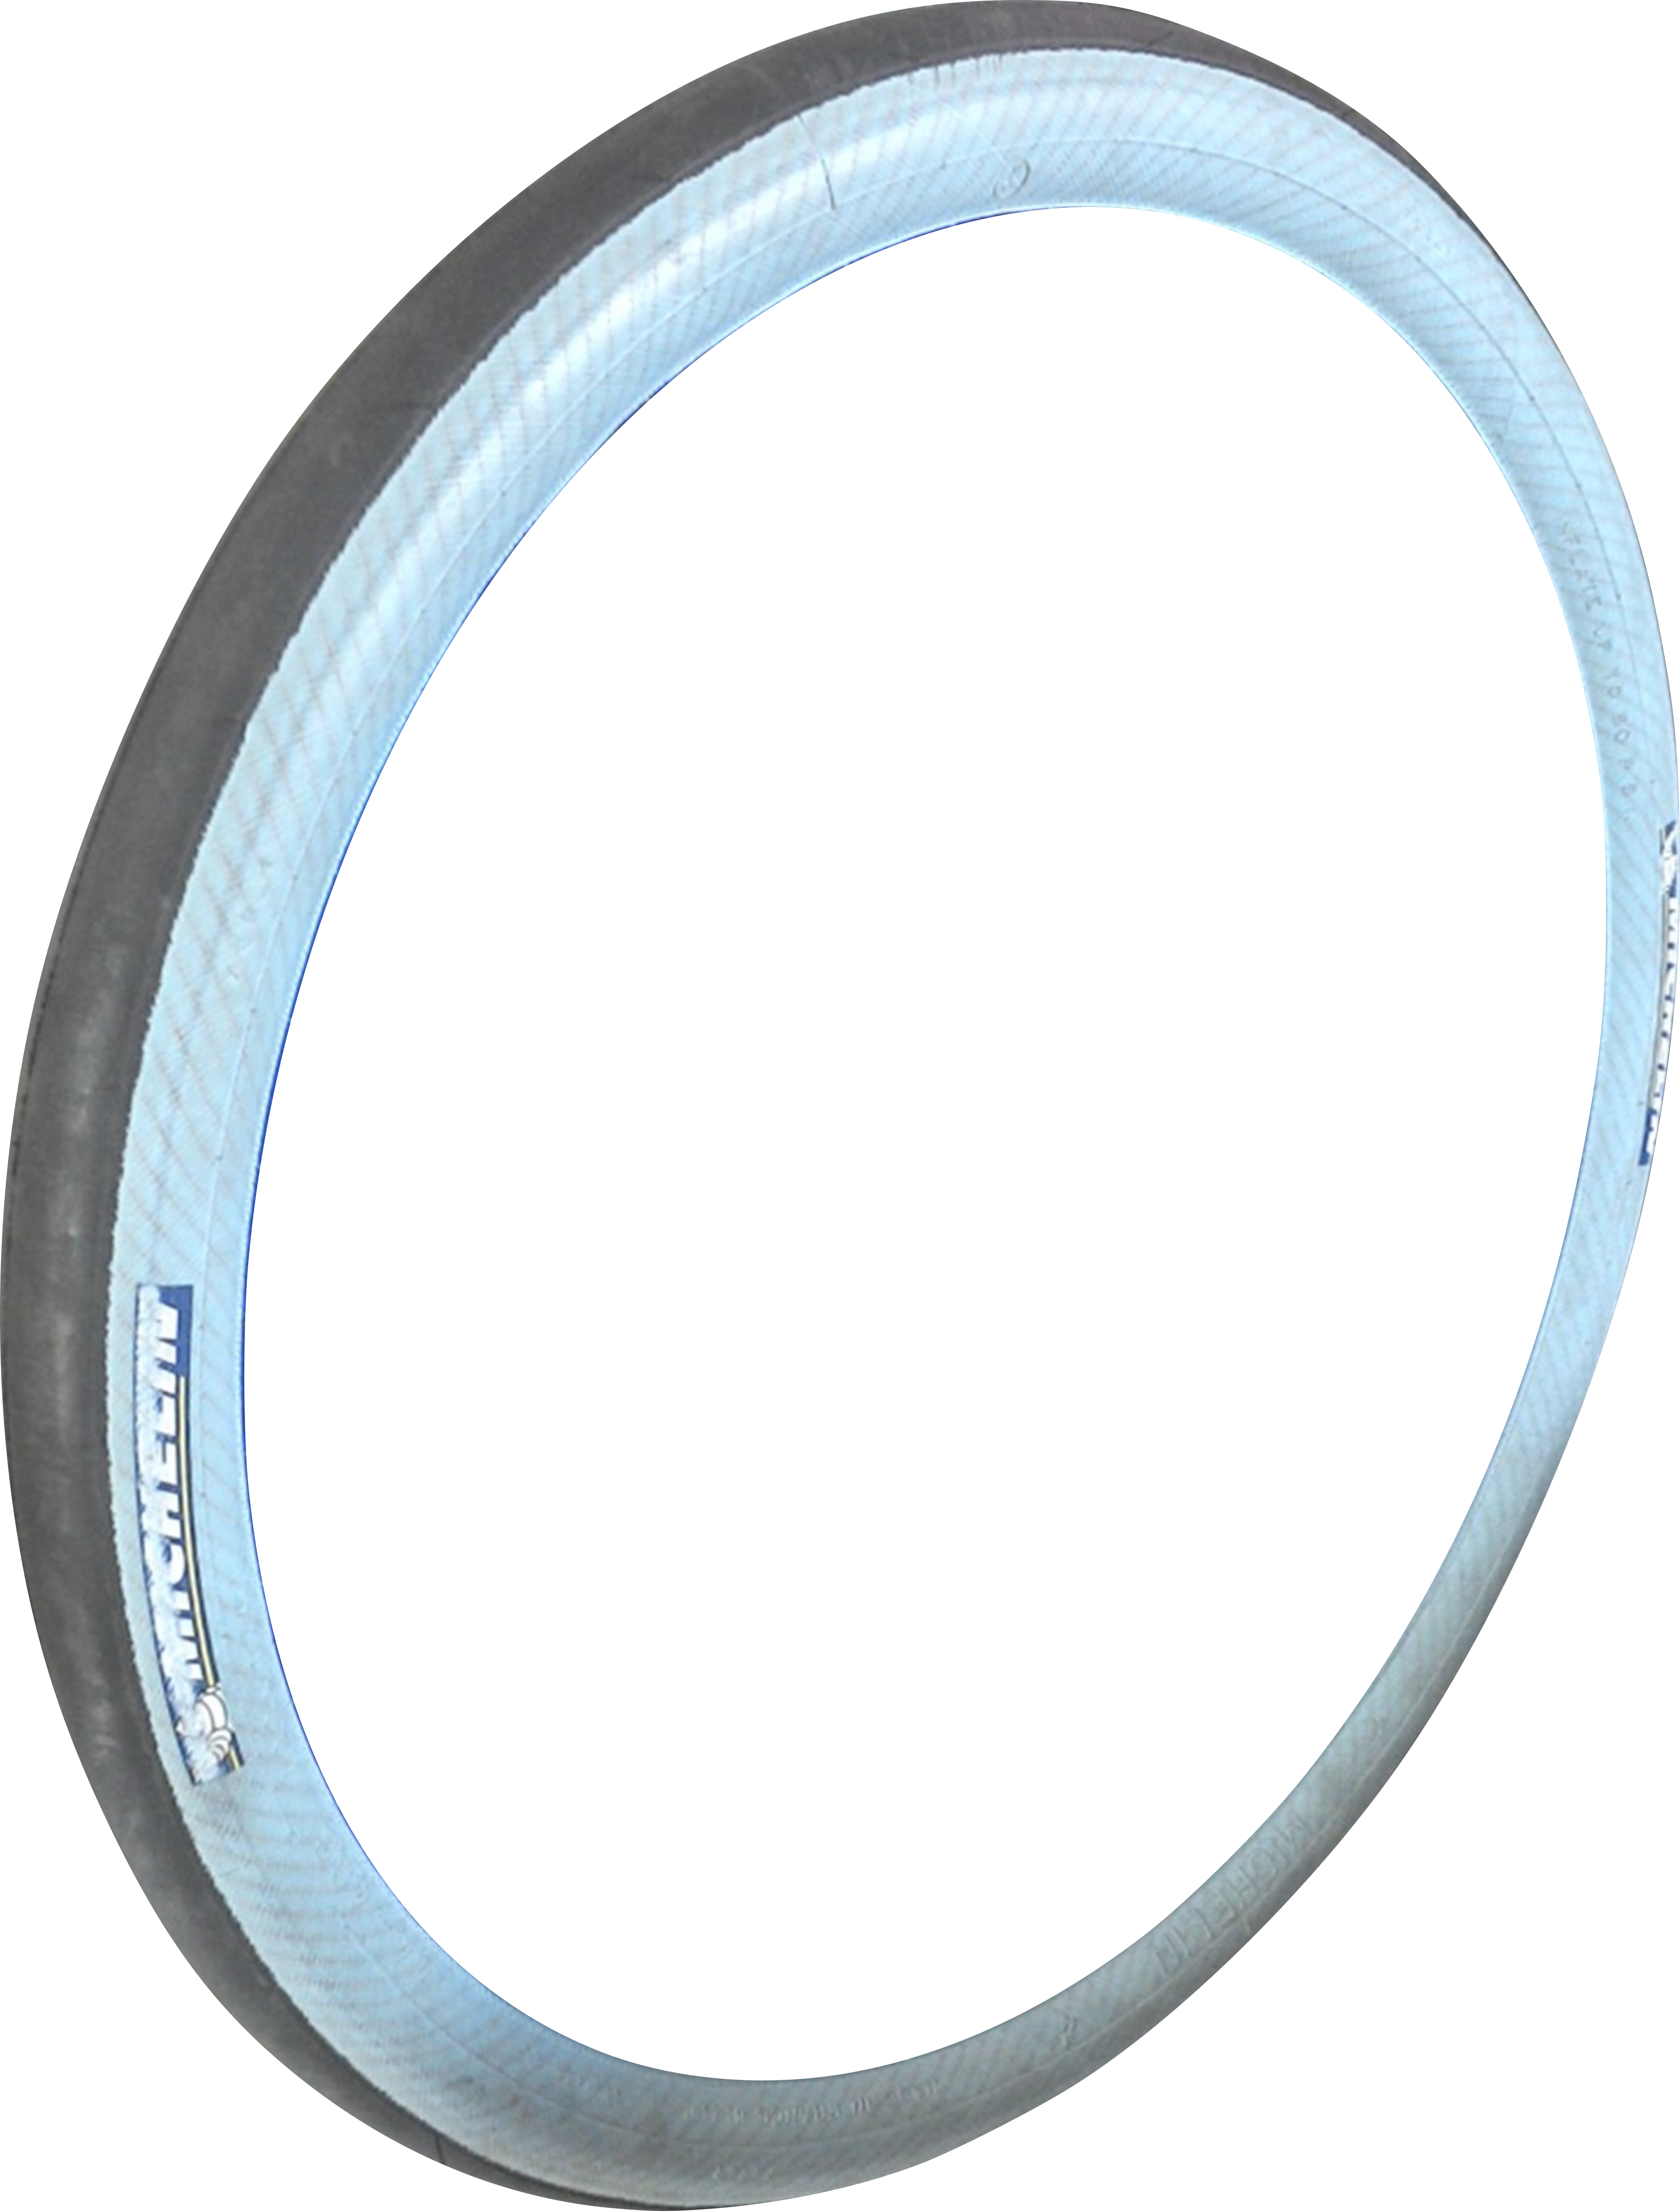
\includegraphics[scale=0.25]{DescricaoProcesso/Figuras/pneu_Michelin.png}
	\caption*{\footnotesize Fonte: Equipe Milhagem UFMG.}
\end{figure}

\subsection{Sistema de propulsão}
\label{subsec:sistema_propulsao}

De forma genérica, o sistema de propulsão de um veículo elétrico, representado no diagrama da Figura \ref{fig:diagrama_propulsao}, é composto por
bateria, conversor de potencia, motor elétrico e transmissão.

\begin{figure}[H]
	\centering
	\caption{Diagrama de blocos do sistema de propulsão de um veículo elétrico}
	\label{fig:diagrama_propulsao}
	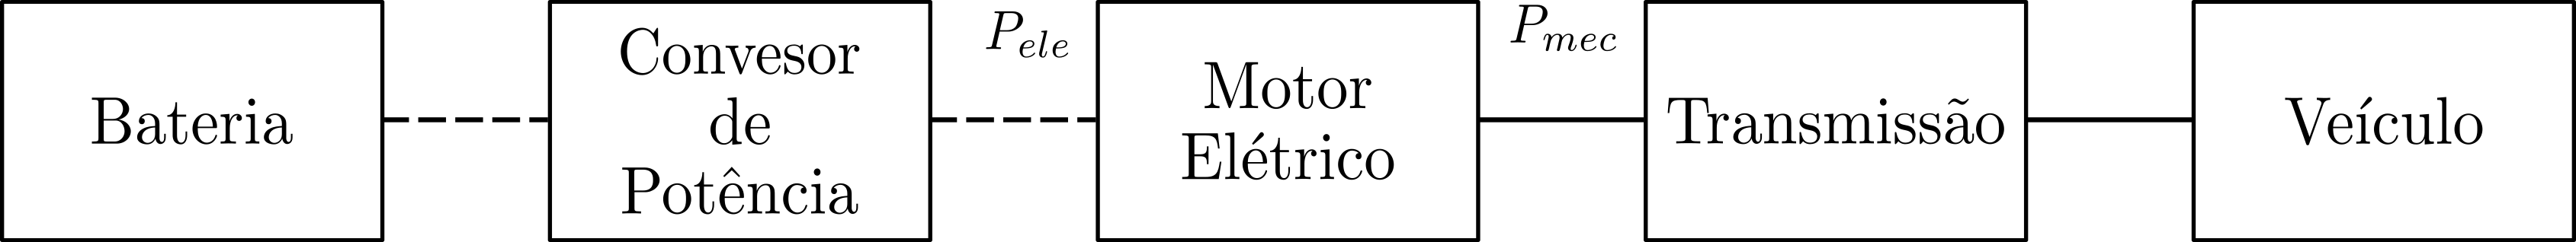
\includegraphics{DescricaoProcesso/Figuras/g874.png}
	\caption*{\footnotesize Fonte: Elaborado pelo autor.}
\end{figure}

\subsubsection{Bateria}

Bateria eletroquímica, ou apenas bateria, é um dispositivo em que durante a descarga ocorre a conversão de energia potencial química em energia
elétrica e na carga ocorre a conversão inversa. Ou seja, uma bateria armazena energia elétrica na forma de energia potencial química. Uma bateria é
composta por varais células ligadas entre se. Uma célula de bateria é basicamente composta por dois eletrodos -- positivo e
negativo -- imersos em um eletrólito\cite{book:Modern_Electric_Vehicles}.

\subsubsection{Conversor de Potência}

Conversor eletrônico de potência, ou conversor de potência, é o circuito cujo a finalidade é extrair energia elétrica de um sistema de energia e
transformá-la em uma forma adequada e necessária para um motor\cite{book:Electric_Motor_Control}.

\subsubsection{Motor Elétrico}

O motor elétrico converte a potencia elétrica -- tensão e corrente -- em potencia mecânica rotativa -- torque e rotação -- para impulsionar o
veículo.\cite{book:Modern_Electric_Vehicles} Podem ser classificados em relação a sua alimentação: corrente continua
(CA) ou corrente alternada (CC), conforme apresentado na Figura \ref{classif_motor}.
No entanto o motor de corrente continua sem escovas, ou BLDC do inglês \textit{brushless direct current}, é difícil de ser classificado desse forma
pois sua configuração é semelhante à de um motor CA, enquanto suas características elétricas são semelhantes às de um motor
CC.\cite{book:Electric_Motor_Control} Nesse trabalho estudara-se o modelo dos motores BLDC pois é o tipo de motor utilizado no protótipo DT1.

\begin{figure}[H]
	\centering
	\caption{Classificação de motores elétricos}
	\label{classif_motor}
	\begin{tikzpicture}[grow'=right,
			level distance=4cm,
			level 1/.style={sibling distance=5cm},
			level 2/.style={sibling distance=1.5cm},
			edge from parent fork right]
		\tikzstyle{every node}=[draw,minimum width=1in,text width=1in,align=center]

		%\draw [help lines] (0,-5) grid (10,5);

		\node (Root) {Motor Elétrico}
		child {
				node {Corrente Continua}
				child { node {Excitação independente} }
				child { node {Auto excitação} }
			}
		child {
				node {Corrente Alternada}
				child { node {Síncrono} }
				child { node {Assíncrono (indução)} }
			};
		\node[draw] at (8, 0)	(a) {BLDC};
		\draw[dashed] (6,2) -- (6,-2);
		\draw[dashed] (6,0) -- (6.55,0);
	\end{tikzpicture}
	\caption*{\footnotesize Fonte: Adaptado de \citeauthor{book:Electric_Motor_Control}}
\end{figure}

O motor BLDC foi desenvolvido em 1962 e possui um sistema de comutação eletrônica ao ives de comutação mecânica como os motores CC. Para não utilizar
as escovas da comutação mecânica, os enrolamentos da armadura são colocados no estator (parte estacionaria) e os ímãs são colocados no rotor (parte
rotativa).
A comutação eletrônica baseia-se em sensores para identificar a posição do rotor e acionar o enrolamento necessário para manter o movimento de
rotação.\cite{book:Electric_Motor_Control} O conjunto de equações que descreve a corrente de armadura $i_a$ e o torque gerado $T$ para um motor BLDC
de enrolamentos ligados em
Y com neutro acessível e operando em meia onda (a tensão é aplicada entre o terminal de um enrolamento e o neutro), Figura \ref{diag:motoBLDC}, é

\begin{subequations}
	\label{eq:MotorCC}
	\begin{align}
		u - u_{ind}  = L_{a} \cdot \dot i_{a} + R_{a} \cdot i_{a}\enspace, \label{eq:MotorCC_1} \\
		u_{ind} = K_{v} \cdot \omega_{m}\enspace, \label{eq:MotorCC_2}                          \\
		T = K_{t} \cdot i_{a}\enspace, \label{eq:MotorCC_3}
	\end{align}
\end{subequations}

em que $u$ é a tensão aplicada, $u_{ind}$ é a tensão induzida, $l_{m}$ e $r_{m}$ são, respectivamente a indutância e a resistência da armadura,
$K_{v}$ é a constante de tensão induzida,
$\omega_{m}$ é a rotação do motor e $K_{t}$ é a constante de torque.\cite{book:Permanent_Magnet_Motor}

\begin{figure}[H]
	\centering
	\caption{Circuito equivalente de um motor BLDC}
	\begin{center}
		\begin{circuitikz}
			%\draw [help lines] (-1,-2) grid (9,5);

			% circuito
			\draw (0,3) to[V, i<^=$i_a$, v_=$u$] (0,0);
			\draw (0,3) to[R, l=$R_A$] (3,3);
			\draw (3,3) to[L, l=$L_A$] (4,3);
			\draw (4,3) -- (5,3);
			\draw (5,3) to[V, v_=$u_{ind}$] (5,0);
			\draw (0,0) -- (5,0);

			% motor
			\draw[fill=black] (4.85,0.85) rectangle (5.15,2.15);
			\draw[fill=white] (5,1.5) ellipse (.45 and .45);

			% eixo
			\draw[fill=black] (5.45,1.45) rectangle (6.8,1.55);

			% rotação e torque
			\draw[line width=0.7pt,<-] (5.8,1) arc (-30:30:1);
			\draw[line width=0.7pt,<-] (6.4,1) arc (-30:30:1);

			% anotações
			\draw (5.85,2.2) node {$\omega_m$};
			\draw (6.4,2.25) node {$T$};
			\draw (4.5, 2.25) node {$+$};
			\draw (4.5, 0.75) node {$-$};
		\end{circuitikz}
	\end{center}
	\label{diag:motoBLDC}
	\caption*{\footnotesize Fonte: Elaborado pelo autor.}
\end{figure}

O prototipo DT1 é equipado com um motor Dunkermotoren BG75x75 40V (Figura \ref{fig:motor_bg75}). O motor que possui 3 enrolamentos, imã de neodímio
com 8 polos e sensor hall integrado para medir a posição do rotor (24 pulsos por volta), suas características elétricas e mecânicas estão
apresentadas na Tabela \ref{tab:dadosBg75}.

\begin{figure}[H]
	\centering
	\caption{Motor Dunkermotoren BG75x75 40V}
	\label{fig:motor_bg75}
	\includegraphics[scale=0.25]{DescricaoProcesso/Figuras/bg75.png}
	\caption*{\footnotesize Fonte: Adaptado de }
\end{figure}

\begin{table}[H]
	\centering
	\caption{Dados do motor BG75x75 40V}
	\label{tab:dadosBg75}
	\rowcolors{1}{}{lightgray}
	\begin{tabular}{lcc}
		\toprule
		Tensão nominal            & {[}V{]}        & 40     \\
		Corrente nominal          & {[}A{]}        & 15,6   \\
		Torque nominal            & {[}N.m{]}      & 150    \\
		Velocidade nominal        & {[}rpm{]}      & 3370   \\
		Troque de atrito          & {[}N.m{]}      & 0,13   \\
		Torque de parada          & {[}N.m{]}      & 12     \\
		Velocidade sem carga      & {[}rpm{]}      & 4100   \\
		Potencia de saída nominal & {[}W{]}        & 530    \\
		Potencia de saída máxima  & {[}W{]}        & 1150   \\
		Constante de torque       & {[}N.m/A{]}    & 0,119  \\
		Resistência               & {[}$\Omega${]} & 0,07   \\
		Indutância                & {[}mH{]}       & 0,45   \\
		Corrente de pico          & {[}A{]}        & 63     \\
		Inercia do rotor          & {[}g.m²{]}     & 0,0625 \\
		Massa                     & {[}kg{]}       & 2,8    \\
		\bottomrule
	\end{tabular}
	\caption*{\footnotesize Fonte: Adaptado de }
\end{table}

\subsubsection{Transmição}

A transmissão do veículo regula a transferência de potência do motor para as rodas. É basicamente composta por mecanismo de
redução -- ex. caixa de câmbio -- e por um mecanismo de interrupção -- ex. embreagem\cite{book:Modern_Electric_Vehicles}.
No DT1, o mecanismo de redução utilizado é do tipo roda de atrito e o mecanismo de interrupção é o pivotamento entre os componentes da roda de atrito (Figura ).

Rodas de atrito são uma das maneiras mais simples para se transmitir potencia mecânica entre eixos. São composta por dois ou mais cilindros em contato direto.  
Para não ocorrer deslizamento em uma roda de atrito o torque transmitido não deve exceder a força de atrito entre os cilindros. A eficiência na transmissão do torque 

\begin{subequations}
	\label{eq:Transmissao}
	\begin{align}
		\varphi = \frac{R_{motor}}{R_{roda}}\enspace, \label{eq:Transmissao_1} \\
		\omega_{roda} = -\frac{\omega_{motor}}{\varphi}\enspace, \label{eq:Transmissao_2}  \\
		T_{roda} =\varphi \cdot T_{motor} \cdot \eta \enspace, \label{eq:Transmissao_3}
	\end{align}
\end{subequations}


\section{Controle Ótimo}

"O objetivo da teoria de controle ótimo é determinar os sinais de controle que farão com que um processo satisfaça as restrições físicas e ao mesmo
tempo minimize
(ou maximize) alguns critérios de desempenho."\cite{book:Kirk}

O seguinte conjunto de equações é uma formulação genérica e comum para um problema de controle ótimo (OCP)

\begin{mini!}
{x(\cdot),u(\cdot)}{\int_{0}^{T} L(x(t),u(t)) \,\mathrm{d}t + E(x(T)) \label{eq:ObjOCP}}
{\label{eq:formulacaoOCP}}{}
\addConstraint{x(0)-x_{0}}{=0 \label{eq:C1_OCP}}{}
\addConstraint{\dot x(t) - f(x(t),u(t))}{=0, \quad}{t \in \left[0,T\right]  \label{eq:C2_OCP}}
\addConstraint{h(x(t),u(t))}{\leq 0, \quad}{t \in \left[0,T\right]  \label{eq:C3_OCP}}
\addConstraint{r(x(T))}{\leq 0 \enspace, \label{eq:C4_OCP}}{}
\end{mini!}

em que a Equação \ref{eq:ObjOCP} é o funcional-objetivo, Equação \ref{eq:C1_OCP} é uma restrição de estados inciais fixos, Equação \ref{eq:C2_OCP} é
a restrição
que representa a dinâmica
do sistema, Equação \ref{eq:C3_OCP} são restrições de caminho sobre os estados do sistema e sobre as variáveis de controle e Equação \ref{eq:C4_OCP}
é uma restrição de espaço para os estados finais.

O funcional-objetivo, também conhecido como objetivo de Bolza, é composto por uma integral de $L(x,u)$ conhecida como termo de Lagrange
e uma função $E(x)$ conhecida como termo de Meyer\cite{book:Numerical_Optimal_Control}.

\begin{figure}[H]
	\centering
	\caption{Exemplo do comportamento desejado das variáveis em um OPC}
	\label{fig:simpleOPC}
	\begin{tikzpicture}
		%\draw [help lines] (-1,-2) grid (12,7);
		\centering
		\begin{axis}[
				width=11cm, height=8cm,
				xmin=0, xmax=15,
				ymin=0, ymax=10,
				xlabel=$t$,
				xtick = {0,15}, xticklabels = {$0$,$T$},
				yticklabels={}]
			\addplot[smooth] plot coordinates {
					(0, 4)
					(2, 4.25)
					(4, 5)
					(6, 7)
					(10, 7)
					(11, 6)
					(12, 5.5)
					(15, 5.3)
				}node[pos=.5, below] {estado $x(t)$};

			\addplot[smooth] plot coordinates {
					(0, 1)
					(2, 1.1)
					(5, 2)
				};
			\addplot[smooth] plot coordinates {
					(5, 2.5)
					(8, 2.8)
					(10, 1.5)
				}node[pos=.5, above] {vari\'{a}vel de controle $u(t)$};
			\addplot[smooth] plot coordinates {
					(10, 0)
					(13, 0)
				};
			\addplot[smooth] plot coordinates {
					(13, 1.5)
					(14, 1.5)
					(15, 0)
				};

			\addplot[dashed, black] coordinates {
					(0,8) (15,8)
				}node[pos=.5, above] {restri\c{c}\~{o}es de caminho $h(x(t),u(t)) \leq 0$};

		\end{axis}
		\filldraw[black] (0,2.57) circle (2pt) node[left] {
				\begin{tabular}{r}
					valor inicial \\$x_0$
				\end{tabular}
			};
		\draw (9.2,3) -- (9.6,3) (9.2,4) -- (9.6,4);
		\draw[dashed,line width=0.75mm] (9.4,3) -- (9.4,4) node[right, pos=.5] {
			\begin{tabular}{l}
				restri\c{c}\~{a}o de \\valor final\\	$r(x(T))\leq 0$
			\end{tabular}
		};
	\end{tikzpicture}
	\caption*{\footnotesize Fonte: Adaptado de }
\end{figure}

\begin{figure}[H]
	\centering
	\caption{Visão geral do métodos numéricos para controle ótimo}
	\label{fig:diagrama_metodos_numericos}
	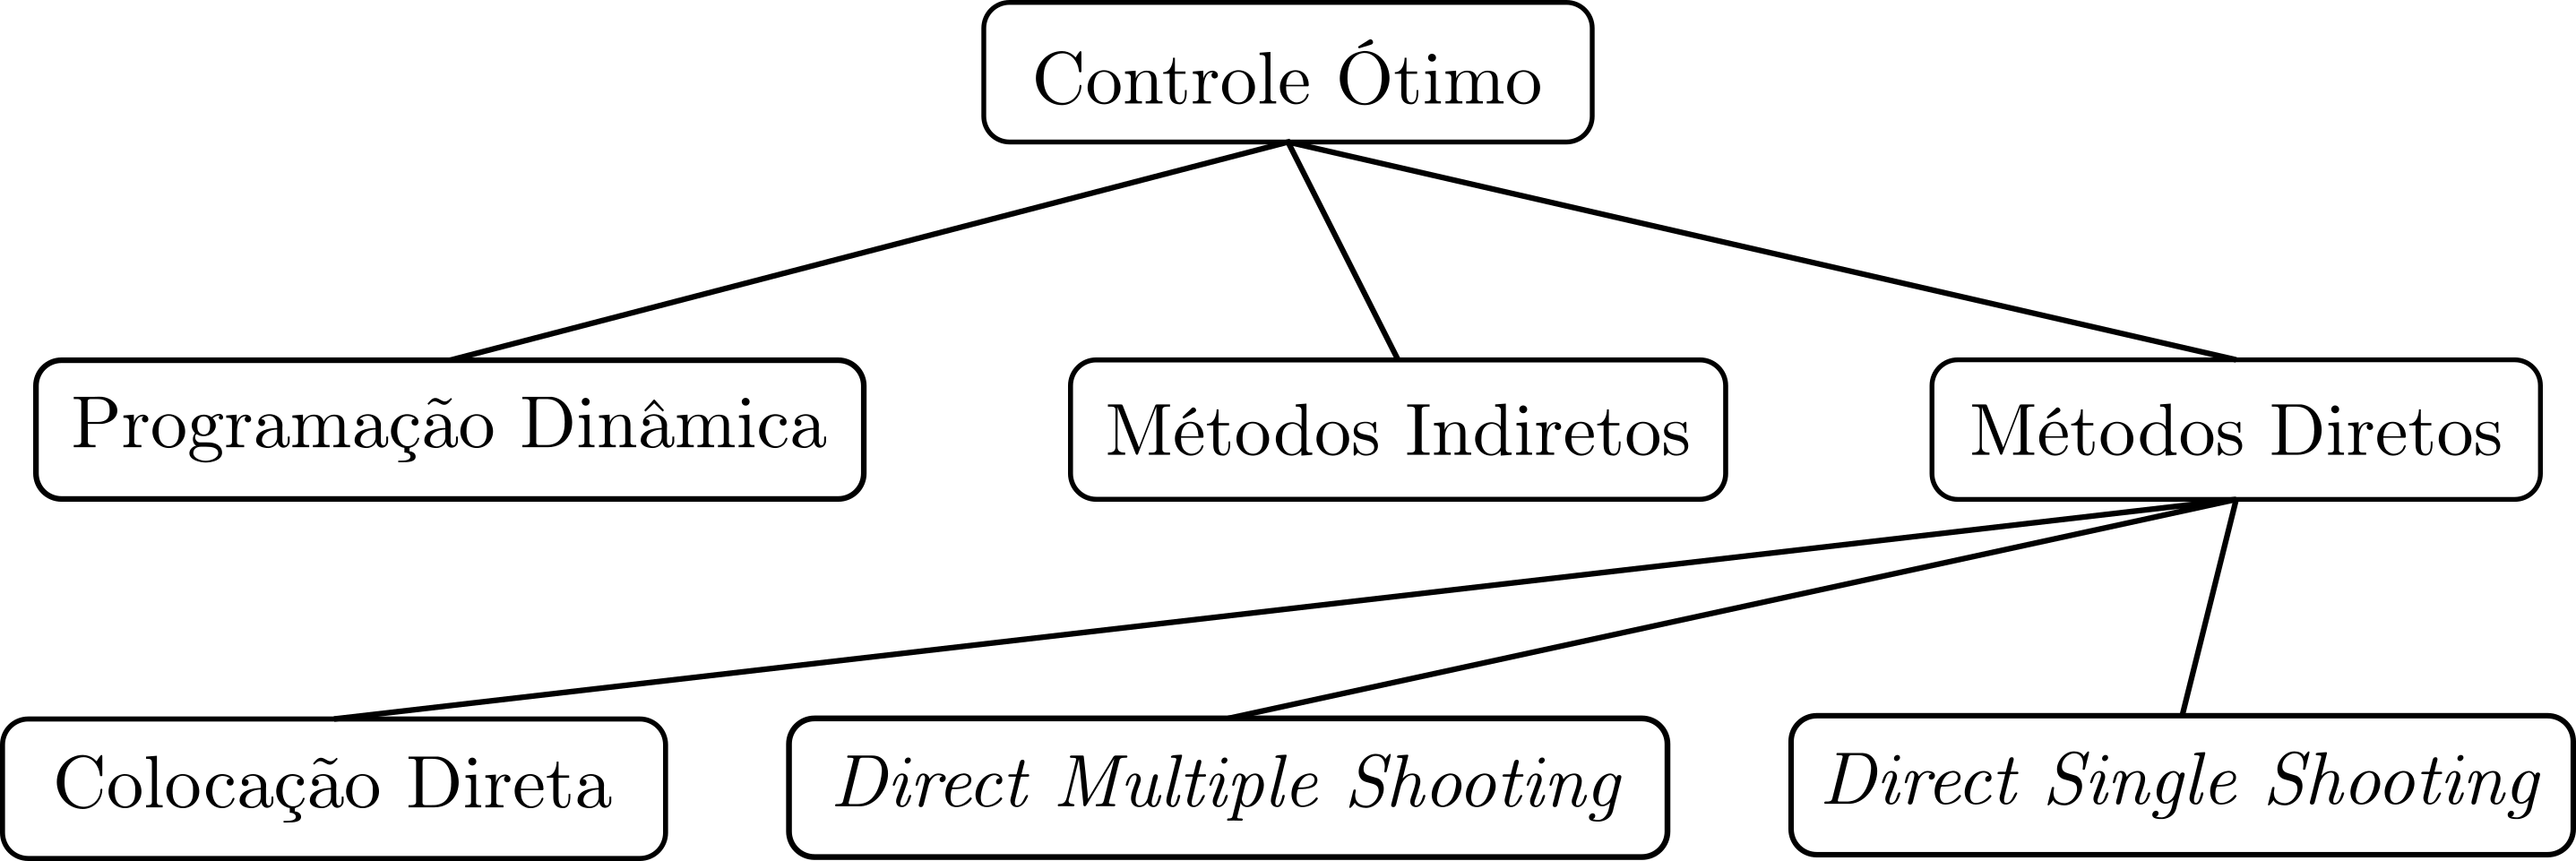
\includegraphics{DescricaoProcesso/Figuras/diagrama_metodos_numericos.png}
	\caption*{\footnotesize Fonte: Adaptado de \citeauthor{article:Diehl}}
\end{figure}

\clearpage
\chapter{Metodologia}
\label{chap:metodologia}
\thispagestyle{empty}

É apresentado neste capítulo o desenvolvimento realizado neste projeto, os problemas encontrados e as soluções propostas.
Na primeira e segunda seção tem-se a definição do modelo matemático do veículo protótipo DT1 e da pista. A terceira seção traz a formulação proposta para o problema de controle ótimo que encontrar
a estratégia de pista ótima. Por fim, na última  seção é apresentado os passos realizados no desenvolvimento do código que soluciona o OCP proposto. 

\section{Modelo do veículo DT1} 

O modelo da dinâmica do veículo protótipo DT1 foi definido com base na revisão bibliográfica apresentada na Seção \ref{sec:modelo}. 
Para isto as seguintes simplificações e considerações foram feita:

\begin{itemize}
    \item \textbf{Dinâmica lateral:} não foi levando em conta a dinâmica lateral do veículo considerando que ele se move apenas em linha reta; 
    \item \textbf{Vento:} a velocidade do vento foi desconsiderada na Equação (\ref{eq:Fa});
    \item \textbf{Pneus:} a variação do coeficiente de rolamento em função da temperatura, da pressão e a velocidade não foi considerada na Equação (\ref{eq:Fr});
    \item \textbf{Rolamentos:} o atrito viscos dos rolamentos foi considerado nulo;
    \item \textbf{Perdas elétricas:} a bateria e o conversor eletrônico de potência foram tratados como componentes ideias não modificações na dinâmica das grandezas elétricas;
    \item \textbf{Indutância do motor:} como a dinâmica da velocidade é pelo menos dez vez mais lenta que a dinâmica da corrente elétrica, a contribuição do  indutor foi removida da Equação (\ref{eq:propulsao_1}).  
\end{itemize}

A partir das Equações (\ref{eq:SomaForcas}) à (\ref{eq:Fr}) e (\ref{eq:propulsao}) e destas simplificações e considerações foi definido a 
seguinte equação para descrever o comportamento do veículo

\begin{subequations}
	\label{eq:modelo_1}
    \begin{align}
        \left( m_v + m_p + N_r \cdot \frac{J_r}{r_r^2}  + \frac{J_m}{r_m^2} \right) \dot v = F_t - (F_a + F_g + F_r) \enspace,\\   
        F_{t} =  \frac{K_t \cdot i_a \cdot \eta}{r_m} \enspace,\\
		R_{a} \cdot i_{a} = u - \frac{K_{v} \cdot v}{r_m} \enspace, \\
        F_{a} = \frac{\rho \cdot a_f \cdot c_d \cdot v^2}{2} \enspace,\\
        F_{g} = (m_v + m_p) \cdot g \cdot \sin(\theta(x)) \enspace,\\
        F_{r}  = c_{r} \cdot (m_v + m_p) \cdot g \cdot \cos(\theta(x)) \enspace,
	\end{align}
\end{subequations}

em que as variáveis são $\dot v$ a aceleração 
do carro em [$m/s^2$], $v$ a velocidade do carro em [$m/s^2$], $x$ a distância  percorrida pelo carro na pista em [$m$], 
$u$ a tensão aplicada no motor em [$V$], $r_m$ o raio do cilindro de transmissão no eixo do motor elétrico em [$m$] e $\theta$ é a inclinação da pista em [$rad$] 
e as constantes estão apresentadas na Tabela \ref{tab:constantes}. Não foi realizado ensaio para determinar ou verificar essas constantes e este modelo
pois o projeto foi realizado, em sua maior parte, durante o Ensino Remoto Emergencial de 2020. As constantes foram definidas através da bibliografia apresentada
e por dados fornecidos pela equipe Milhagem UFMG. 

% em que as variáveis são $u$ a tensão aplicada no motor em [$V$], 
% $r_m$ o raio do cilindro de transmissão no eixo do motor em [$m$], 
% $\theta$ é a inclinação da pista em [$rad$], $\dot v$, $v$ e $x$ são respectivamente a aceleração em [$m/s^2$], a velocidade em [$m/s$] e posição [$m$] do carro
% e as constantes estão apresentadas na Tabela \ref{tab:constantes}. Não foi realizado ensaio para determinar ou verificar essas constantes ou este modelo
% pois o projeto foi realizado, em sua maior parte, durante o Ensino Remoto Emergêncial. As constantes foram definidas através da bibliografia apresentada
% e por dados fornecidos pela equipe Milhagem UFMG. 

\begin{table}[H]
	\centering
	\caption{Constantes utilizadas no modelo do veículo}
	\rowcolors{1}{}{lightgray}
	\begin{tabular}{llll}
		\toprule
		\textbf{Constante} & \textbf{Simbolo} & \textbf{Unidade} & \textbf{Valor}\\
		\hline
		Massa veículo                       & $m_v$  & [$kg$]              & 36      \\
        Massa do piloto                     & $m_p$  & [$kg$]              & 50      \\
        Resistência de armadura             & $R_a$  & [$\Omega$]        & 0,07    \\  
        Const. de tensão induzida           & $K_v$  & [$V/(rad/s)$]       & 0,119   \\
        Quantidade de rodas                 & $N_r$  & [ ]                & 3       \\
        Momento de inercia da roda          & $J_r$  & [$kg.m^2$]        & 0,015   \\
        Momento de inercia do motor         & $J_m$  & [$kg.m^2$]        & $0,0625 \times 10^{-3}$\\
        Raio da roda                        & $r_r$  & [$m$]               & 0,254   \\
        Const. de torque                    & $K_t$  & [$Nm/A$]            & 0,119   \\
        Eficiência da roda de atrito        & $\eta$ & [ ]                & 0,95    \\
        Densidade do ar                     & $\rho$ & [$kg/m^3$]        & 1,22    \\
        Areá fronta do veículo              & $a_f$  & [$m^2$]           & 0,26    \\
        Coef. de arrasto aerodinâmico       & $c_d$  & [ ]                & 0,164   \\
        Aceleração da gravidade             & $g$    & [$m/s^2$]         & 9,81    \\
        Coef. de resistência ao rolamento   & $c_r$  & [ ]                & 0,0024  \\
		\bottomrule
	\end{tabular}
	\caption*{\footnotesize Fonte: Elaborada pelo autor.}
	\label{tab:constantes}
\end{table}


\section{Modelo da pista}

Para obter os dados de altitude da pista da Shell Eco-marathon Americas de 2019 no Kartódromo de Sonoma foi feito uma requisição a equipe
\textit{Duke Electric Vehicles} da \textit{Duke University} que disponibilizou os dados coletados e tratos por ela. A Figura apresentada \ref{fig:altitude_pista} 
o perfil de altitude da pista com estes dados.

\begin{figure}[h]
    \centering
    \caption{Perfil de altitude da pista da Shell Eco-marathon Americas de 2019}
    % This file was created by matlab2tikz.
%
%The latest updates can be retrieved from
%  http://www.mathworks.com/matlabcentral/fileexchange/22022-matlab2tikz-matlab2tikz
%where you can also make suggestions and rate matlab2tikz.
%
\definecolor{mycolor1}{rgb}{0.00000,0.44700,0.74100}%
%
\begin{tikzpicture}[scale=0.75]

\begin{axis}[%
width=4.521in,
height=3.566in,
at={(0.758in,0.481in)},
scale only axis,
xmin=0,
xmax=1500,
xlabel style={font=\color{white!15!black}},
xlabel={distância  ao longo da pista [m]},
ymin=-2,
ymax=5,
ylabel style={font=\color{white!15!black}},
ylabel={Altitude relativa [m]},
axis background/.style={fill=white},
xmajorgrids,
ymajorgrids
]
\addplot [color=mycolor1, forget plot]
  table[row sep=crcr]{%
0	0\\
5.12221633837888	0.0357379396676334\\
10.0516199164945	0.104972074967328\\
15.1016863618342	0.107722115067246\\
20.0557383939357	0.143408459194609\\
25.0180390039261	0.185390922437452\\
30.0994558692112	0.242808963848907\\
35.0194754612144	0.265343842059095\\
40.1032362448675	0.306213896817238\\
45.0302720648865	0.34432100835364\\
50.0199618336967	0.363243823798147\\
55.0601872298759	0.408402295729659\\
60.081861665023	0.448736973032622\\
65.0034315382065	0.507448710411661\\
70.0133461222134	0.528655675550714\\
75.0427696663329	0.548738481850909\\
80.0289031360195	0.580077859552539\\
85.0540374361473	0.603092814287619\\
90.0039519341915	0.647564873838286\\
95.0344626775333	0.699131894236861\\
100.08412719663	0.734374644606736\\
105.087949763056	0.776654148548195\\
110.029320108579	0.801470868883285\\
115.109002769075	0.830801204323592\\
120.047990525275	0.859470217807589\\
125.077509699709	0.91471428857013\\
130.043700015891	0.986995023844734\\
135.057777483852	1.04455129324355\\
140.023845274091	1.12650442548788\\
145.067814961286	1.1975924169145\\
150.071951699855	1.29765754647297\\
155.067333935021	1.42611842181642\\
160.046476069651	1.55343586345637\\
165.024396395583	1.70034960164136\\
170.059139443888	1.81757768174917\\
175.033685409674	1.83842327477578\\
180.100556336227	1.88992242741691\\
185.093553265802	1.95895970651273\\
190.075606815513	2.00573333352113\\
195.072302587681	2.00650260273968\\
200.084744663884	2.1076074957122\\
205.046000450717	2.21707009877046\\
210.03864921318	2.36430784814989\\
215.098558493801	2.52909944692323\\
220.067805214036	2.68727014749316\\
225.104324773213	2.84193460225021\\
230.05185929419	3.03165841315539\\
235.077383866855	3.15829537724148\\
240.017508877014	3.27837165636326\\
245.005808937912	3.42016227481439\\
250.015268947595	3.52188807387367\\
255.050892541585	3.60834889388607\\
260.0063277381	3.68748899725192\\
265.001156445286	3.80818363772489\\
270.070454536791	3.95485125560833\\
275.015227568311	4.08844028589769\\
280.07919560007	4.22764024171798\\
285.072102690404	4.32337923819937\\
290.088508702335	4.42913326069625\\
295.020995241378	4.48294754669859\\
300.057050371967	4.54487313347786\\
305.071971070169	4.60995547396562\\
310.067857483967	4.6480347286057\\
315.047026372111	4.67283089060249\\
320.011218889021	4.6916842630321\\
325.045486563677	4.73623001881343\\
330.005090294992	4.73121711204915\\
335.084013035874	4.74915299856471\\
340.005128438622	4.76033344145669\\
345.046186095374	4.70260303614258\\
350.059781945331	4.66277010581372\\
355.037249011958	4.56879524739148\\
360.088602713913	4.39077246022415\\
365.046961987169	4.17467114933649\\
370.01071293774	3.95628631039429\\
375.04960497426	3.75611837613893\\
380.013235457204	3.5983623827951\\
385.010028062919	3.53529426275642\\
390.024258467701	3.46152316489486\\
395.073752715841	3.4504967877954\\
400.100767589134	3.4657282840199\\
405.044216785212	3.50316296864385\\
410.046252351497	3.45107272053722\\
415.003397910249	3.39522146375892\\
420.068346926989	3.36561232213679\\
425.00814024125	3.27320493082273\\
430.018228184296	3.19784489867244\\
435.033185395297	3.17867482035181\\
440.062335167934	3.36366439572127\\
445.067880453611	3.67678539727011\\
450.112944370747	4.02373555328033\\
455.11403031075	4.32732894090232\\
460.031288489432	4.56208775403152\\
465.01377484305	4.74555059404158\\
470.094421755121	4.83813648123462\\
475.007478345653	4.81994370474145\\
480.093488339411	4.8294559666483\\
485.000116654387	4.8345701495991\\
490.093619430145	4.80574940639705\\
495.087218007541	4.72226349670508\\
500.086065915516	4.63320429294828\\
505.104190099561	4.54126835063877\\
510.019711436402	4.46206553739806\\
515.048889261962	4.31136925109454\\
520.050480466514	4.21620789363706\\
525.012290421834	4.13402072221267\\
530.040185205617	4.06237307599751\\
535.013378599529	3.99088064611747\\
540.003754990435	3.93460579828708\\
545.081387320683	3.85947030304406\\
550.11616167678	3.80514844662332\\
555.10335455619	3.7335202568295\\
560.090760735292	3.65628812843982\\
565.018483478686	3.59900863087375\\
570.063865000408	3.55724806163802\\
575.087323611412	3.51314509373265\\
580.07577584618	3.43907631088358\\
585.003009891568	3.35668016868912\\
590.013775544679	3.27571958492176\\
595.053529786038	3.23793714976627\\
600.023704620358	3.16736800714642\\
605.081284173436	3.08484077108421\\
610.024102859829	2.99222287368472\\
615.003442302492	2.94648330432707\\
620.019195038574	2.85930067853677\\
625.106885313401	2.76507427978904\\
630.079658274351	2.69969907593198\\
635.079625831954	2.61986156018748\\
640.018038586473	2.52039761917368\\
645.040866697825	2.41451099895905\\
650.067821212943	2.32463779545542\\
655.003093402256	2.21811729440853\\
660.057310505983	2.11457052992626\\
665.023052254712	2.03802093262931\\
670.058568408263	1.94486754473429\\
675.053678819237	1.89254797025235\\
680.089975845145	1.80918873004759\\
685.080739434188	1.70896309716183\\
690.039547759312	1.66520815629269\\
695.04128133922	1.58163176026549\\
700.01571840371	1.48361138379975\\
705.100318245575	1.42705947673011\\
710.019961384519	1.32367399862178\\
715.004297485676	1.21468583866631\\
720.109323670961	1.17472385243005\\
725.084032125554	1.06928976180669\\
730.023660108317	0.97829622998816\\
735.020965856036	0.873257703766727\\
740.005772883376	0.800793016734662\\
745.055880794773	0.675465616374825\\
750.08620183061	0.616332205593579\\
755.063882098672	0.531733627663317\\
760.079998487305	0.425911531812245\\
765.00088746981	0.384668536036159\\
770.100450999183	0.250972178052027\\
775.036344554228	0.185002672519197\\
780.100972351368	0.0944669917970231\\
785.110777356283	0.00424681786595187\\
790.014199541226	-0.0877488857035857\\
795.031774748258	-0.151269250674299\\
800.038746459351	-0.197911047695362\\
805.05940463916	-0.298606267166549\\
810.069922249436	-0.354147137463012\\
815.011285342744	-0.436415813148143\\
820.070273291529	-0.500705315325784\\
825.049129224306	-0.516697795689539\\
830.078334479066	-0.562586602466058\\
835.079917061121	-0.610495075536122\\
840.010310427578	-0.644306068445897\\
845.07792109013	-0.664970855281195\\
850.113021601948	-0.677655324069427\\
855.070006367424	-0.703860435330877\\
860.021479776857	-0.699585417456964\\
865.100283344574	-0.700075425590552\\
870.020283889233	-0.726123522598239\\
875.090901709233	-0.755029496513072\\
880.106208036219	-0.74511641673366\\
885.039935288171	-0.727018970914558\\
890.058500773151	-0.722186723565405\\
895.006123352769	-0.741774912437538\\
900.035076834166	-0.746446244295468\\
905.090735591922	-0.781833160047785\\
910.064264483581	-0.792282145661944\\
915.010308889022	-0.790591647249885\\
920.110660510359	-0.804983218867607\\
925.000057748328	-0.81387796395538\\
930.087286174934	-0.821078712745179\\
935.081959695617	-0.854342056420616\\
940.083370727433	-0.870369930688935\\
945.023076471185	-0.889801875533173\\
950.107469060826	-0.917110565222884\\
955.001696634935	-0.941004986463057\\
960.015704709223	-0.959084187968011\\
965.006099584317	-0.972591040045769\\
970.066311968145	-0.997699227028884\\
975.021311554673	-1.00210603527331\\
980.023935653497	-1.02050010358338\\
985.0557115927	-1.03001588832064\\
990.065339116062	-1.0474959859586\\
995.087140728748	-1.04881847398743\\
1000.11285386713	-1.06068643764929\\
1005.03101498249	-1.06025858866119\\
1010.05869005492	-1.07621878989248\\
1015.01960887244	-1.08990079418245\\
1020.06220081832	-1.08646689527809\\
1025.01707253991	-1.12333716493696\\
1030.00297566732	-1.10569017773104\\
1035.08298560737	-1.13088720503955\\
1040.05671127273	-1.15161012323982\\
1045.06760175857	-1.13333843294349\\
1050.09200275284	-1.13056775279367\\
1055.0337580459	-1.13431715900329\\
1060.07859805313	-1.14957175665922\\
1065.01880107785	-1.2184672627233\\
1070.05067138596	-1.29399145326404\\
1075.06739191434	-1.3496454433149\\
1080.10731907944	-1.41333750417389\\
1085.05830526203	-1.47889231260441\\
1090.06332613413	-1.47779420150597\\
1095.06083863951	-1.46194482553275\\
1100.0155023143	-1.40645504732296\\
1105.00814784638	-1.33620982389129\\
1110.09964467657	-1.27117524821844\\
1115.10402310126	-1.23738812041945\\
1120.06585797096	-1.16852843923131\\
1125.06998177916	-1.09857014264178\\
1130.03989431487	-1.00406079298401\\
1135.0046876791	-0.923322197955167\\
1140.00092053022	-0.880226149213422\\
1145.06584140678	-0.914932604927785\\
1150.10441017199	-0.999495113766608\\
1155.01642846417	-1.04913338491673\\
1160.08008576993	-1.15724500731527\\
1165.04400368188	-1.23524918477314\\
1170.09655572421	-1.29253981852399\\
1175.04634875881	-1.25432433005151\\
1180.0747507166	-1.28885430740302\\
1185.10101425169	-1.24240287439272\\
1190.06633644638	-1.20071987552745\\
1195.03322734328	-1.1523639426173\\
1200.07252895776	-1.07111757257261\\
1205.02773236319	-1.08181865955013\\
1210.01366466762	-1.06827008647517\\
1215.08807911301	-1.07430468531357\\
1220.01367957885	-1.06065222673203\\
1225.02091257449	-1.04657795625494\\
1230.10758634789	-1.04686564225696\\
1235.07298541367	-1.04902302468824\\
1240.02914031163	-1.05056387902854\\
1245.01024457689	-1.06742413773579\\
1250.04723544874	-1.07038841007536\\
1255.06983097477	-1.02475451501524\\
1260.08320135719	-1.03256570030218\\
1265.00193720948	-1.01054464670626\\
1270.08131455567	-0.994223191541616\\
1275.03935496426	-0.980185167817517\\
1280.06757029612	-0.938386124695866\\
1285.04672980522	-0.934087633864927\\
1290.08554681933	-0.920352338366993\\
1295.07741776746	-0.917402124918478\\
1300.02553175819	-0.934915504004597\\
1305.08298789323	-0.912389354524508\\
1310.05439673914	-0.896608327073881\\
1315.05207271433	-0.850469572128962\\
1320.1122572406	-0.816591871675576\\
1325.05104362104	-0.766240094292945\\
1330.06920105181	-0.782409795667201\\
1335.00713872223	-0.771164708786958\\
1340.1044526585	-0.734420905253737\\
1345.07366591704	-0.714223134495311\\
1350.01768337595	-0.704229603660398\\
1355.01060864161	-0.665559200367077\\
1360.08583062332	-0.639871651449299\\
1365.10063454942	-0.606048874273892\\
1370.01713527779	-0.597891199712674\\
1375.04107249332	-0.547816241396431\\
1380.04884560394	-0.495825279060784\\
1385.00445136726	-0.460338726096202\\
1390.02283826446	-0.418375494281441\\
1395.07601543318	-0.362995995067974\\
1401.94143963255	-0.32049007615395\\
1406.26897648743	-0.287264745376155\\
1410.59732430282	-0.25817957036593\\
1415.09024756453	-0.229638711479017\\
1420.0334666681	-0.17511941675372\\
1425.04296595411	-0.124723774183674\\
1430.10690463865	-0.102871966436186\\
1435.05728385009	-0.0481843051562433\\
1440.0152027299	-0.0130804853312747\\
};
\end{axis}

\begin{axis}[%
width=5.833in,
height=4.375in,
at={(0in,0in)},
scale only axis,
xmin=0,
xmax=1,
ymin=0,
ymax=1,
axis line style={draw=none},
ticks=none,
axis x line*=bottom,
axis y line*=left
]
\end{axis}
\end{tikzpicture}%
    \label{fig:altitude_pista}
    \caption*{\footnotesize{Fonte: Dados da equipe de competição \textit{Duke Electric Vehicles}.}}
\end{figure}

Uma forma de representar esses dados no código para solução o OCP é por meio de uma \textit{lookup table} porem ao implementar os dados dessa foram
a solução não convergiu. Uma possível explicação para essa não convergência é que os dados eram derivados duas vezes, uma para determinar a inclinação e outra pelo 
realizada algorítimo de otimização e ao analisar esses dados derivados usando o comando \lstinline[style=Matlab-editor]{diff} do MATLAB  foram observadas curvas
com grande variação de inclinação e ruido. Alem disso seria preciso repetir sete vezes os dois vetores de dados para emular as repetidas voltas realiza pelo carro durante a tentativa.
A solução para esses problemas foi aproximar a curva de altitude da pista por uma sona de senos com o comando \lstinline[style=Matlab-editor]{fit(x, h, 'sin8')} do MATLAB  
e então realizar a derivada para obter a seguinte equação inclinação:

\begin{equation}
	\label{eq:modeloTheta}
	\theta(x) = arctg \left( \sum_{n = 1}^{8} + a_n \cdot cos(b_n \cdot x + c_n) \right)
	\enspace,
\end{equation}

% \begin{table}[H]
% 	\centering
% 	\caption{Ceficientes da Equação (\ref{eq:modeloTheta})}
% 	\rowcolors{1}{}{lightgray}
% 	\begin{tabular}{crcr}
% 		\toprule
% 		\textbf{Coef.} & \textbf{Valor} & \textbf{Coef.} & \textbf{Valor}\\
% 		\hline
% 		$a_1$   & 0,012293 & $a_5$   & 0,003958  \\
%         $b_1$   & 0,004363 & $b_5$   & 0,017449  \\
%         $c_1$   &-0,228758 & $c_5$   &-3,058604  \\  
%         $a_2$   & 0,003041 & $a_6$   & 0,005365  \\
%         $b_2$   & 0,000236 & $b_6$   & 0,026184  \\
%         $c_2$   & 0,399758 & $c_6$   & 0,579933  \\
%         $a_3$   & 0,005818 & $a_7$   & 0,004361  \\
%         $b_3$   & 0,008726 & $b_7$   & 0,021814  \\
%         $c_3$   &-2,193381 & $c_7$   & 1,627015  \\
%         $a_4$   & 0,002926 & $a_8$   & 0,005539  \\
%         $b_4$   & 0,000246 & $b_8$   & 0,030552  \\
%         $c_4$   & 3,490690 & $c_8$   &-1,400496  \\
% 		\bottomrule
% 	\end{tabular}
% 	\caption*{\footnotesize Fonte: Elaborada pelo autor.}
% 	\label{tab:coeficientes}
% \end{table}

\begin{table}[H]
	\centering
	\caption{Coeficientes da Equação (\ref{eq:modeloTheta})}
	\rowcolors{1}{}{lightgray}
	\begin{tabular}{crcrcrcr}
		\toprule
		\textbf{Coef.} & \textbf{Valor} & \textbf{Coef.} & \textbf{Valor} & \textbf{Coef.} & \textbf{Valor} & \textbf{Coef.} & \textbf{Valor}\\
		\hline
        $a_1$   & 0,012293 & $a_3$   & 0,005818 & $a_5$   & 0,003958 & $a_7$   & 0,004361  \\
        $b_1$   & 0,004363 & $b_3$   & 0,008726 & $b_5$   & 0,017449 & $b_7$   & 0,021814  \\
        $c_1$   &-0,228758 & $c_3$   &-2,193381 & $c_5$   &-3,058604 & $c_7$   & 1,627015  \\
        $a_2$   & 0,003041 & $a_4$   & 0,002926 & $a_6$   & 0,005365 & $a_8$   & 0,005539  \\
        $b_2$   & 0,000236 & $b_4$   & 0,000246 & $b_6$   & 0,026184 & $b_8$   & 0,030552  \\
        $c_2$   & 0,399758 & $c_4$   & 3,490690 & $c_6$   & 0,579933 & $c_8$   &-1,400496  \\
		\bottomrule
	\end{tabular}
	\caption*{\footnotesize Fonte: Elaborada pelo autor.}
	\label{tab:coeficientes}
\end{table}


\section{Problema de controle ótimo (OCP)}
\label{sec:OCPporposto}

Utilizando a formulação genérica de OCP da Equação (\ref{eq:formulacaoOCP}), o modelo do veículo dado pela Equação (\ref{eq:modelo_1})
e o manual de regras de competição da Shell EcoMarathon Américas de 2019 
foi definida a seguinte formulação para o problema de controle ótimo de encontrar a estratégia de pista que minimiza o consumo de energia

\begin{mini!}
	{i(t), r_m, T}{\int_{0}^{T} i(t) \cdot [i(t) \cdot Ra + Kv \cdot (v(t)/r_m)] \,\mathrm{d}t \label{eq:ObjOCP_final}}
	{\label{eq:formulacaoOCP_final}}{}
    \addConstraint{x(0)}{=0 \label{eq:C1_OCP_final}}{}
    \addConstraint{v(0)}{=0 \label{eq:C2_OCP_final}}{}
    \addConstraint{\dot x(t) - v(t)}{=0, \quad}{t \in \left[0,T\right]  \label{eq:C3_OCP_final}}
    \addConstraint{\dot v(t) - \frac{F_t - (F_a + F_g + F_r)}{M}}{=0, \quad}{t \in \left[0,T\right]  \label{eq:C4_OCP_final}}
	\addConstraint{i(t)-\frac{42-Kv\cdot(v/r_m)}{R_a}}{\leq 0, \quad}{t \in \left[0,T\right]  \label{eq:C5_OCP_final}}
    \addConstraint{0 \leq i(t)}{\leq 30, \quad}{t \in \left[0,T\right]  \label{eq:C6_OCP_final}}
    \addConstraint{0 \leq v(t)}{\leq 12.5, \quad}{t \in \left[0,T\right]  \label{eq:C7_OCP_final}}
    \addConstraint{x(T)}{= 10080 \label{eq:C8_OCP_final}}{}
	\addConstraint{T}{\leq 1400 \label{eq:C9_OCP_final}}{}
	\addConstraint{0.020\leq r_m}{ \leq 0.050, \label{eq:C10_OCP_final}}{}
\end{mini!}

em que a Equação (\ref{eq:ObjOCP_final}) define a energia elétrica consumida como custo a ser minimizado, 
as Equações (\ref{eq:C1_OCP_final}) e (\ref{eq:C2_OCP_final}) são restrições para os estados iniciaisde distância  percorrida e velocidade nulos, 
as Equações (\ref{eq:C3_OCP_final}) e (\ref{eq:C4_OCP_final}) são as restrições que garantem que os estados da reposta repeitem a dinâmica do modelo da Equação (\ref{eq:modelo_1}), 
a Equação (\ref{eq:C5_OCP_final}) é uma restrição de caminho para corrente em razão da tensão máxima da bateria, 
a Equação (\ref{eq:C6_OCP_final}) é uma restrição para o valor máximo de corrente em função do limite de corrente entregue pelo conversor de potência do veículo,
a Equação (\ref{eq:C7_OCP_final}) é uma restrição para o valor máximo da velocidade do carro definida pela organização da competição,
a Equação (\ref{eq:C8_OCP_final}) é um restrições de valor final fixo para a distância  percorrida equivalente a sete voltas na pista,
a Equação (\ref{eq:C9_OCP_final}) é uma restrição para o valor máximo do tempo final em decorrência do limite de velocidade media mínima determinado pela organização da competição,
e a Equação (\ref{eq:C10_OCP_final}) é o intervalo possível para o raio do eixo do motor.


\begin{table}[H]
	\centering
	\caption{Constantes utilizadas no OCP}
	\rowcolors{1}{}{lightgray}
	\begin{tabular}{llll}
		\toprule
		\textbf{Constante} & \textbf{Simbolo} & \textbf{Unidade} & \textbf{Valor}\\
		\hline
		Tensão da bateria   & $u_{bat}$     & [$V$]    & 42    \\
        Corrente máxima     & $I_{max}$     & [$A$]    & 30    \\
        Velocidade máxima   & $v_{max}$     & [$m/s$]  & 12,5  \\  
        Distância total     & $x_f$         & [$m$]    & 10080 \\
        Tempo final         & $t_f$         & [$s$]    & 1400  \\
        Raio minimo         & $r_{m,min}$   & [$m$]    & 0,02  \\
        Raio máxima         & $r_{m,max}$   & [$m$]    & 0,05  \\
		\bottomrule
	\end{tabular}
	\caption*{\footnotesize Fonte: Elaborada pelo autor.}
	\label{tab:constantes_OCP}
\end{table}

\section{Código para solução do OCP}
\label{sec:metodologia_codigos}

Nesta etapa do trabalho a versão do MATLAB  utilizada foi a R2019b Update 7 e a versão do FALCON.m utilizada foi a v1.26.
O compilador MinGW-w64 C/C++, pré-requisito da biblioteca FALCON, foi instalado gratuitamente na versão 19.2.0 pela loja de aplicativos do MATLAB . 
A licença do MATLAB  utilizada foi a licença acadêmica fornecida pela UFMG à seus alunos. Já a licença do FALCON.m, de uso individual e intransferível,
foi obtida por meio de solicitação feita ao \textit{Institute of Flight System Dynamics} da \textit{Technische Universit{\"a}t M{\"u}nchen} pelo site \url{https://www.fsd.lrg.tum.de/software/falcon-m/license-and-download/}.

A implementação do código para solução do problema de controle ótimo proposto segui os seguintes passos:

\begin{enumerate}
    \item \textbf{Definir as variáveis de estado e de controle e os parâmetros:} no arquivo principal, do tipo \textit{script}, instanciar as  as variáveis de estado e de controle e os parâmetros otimizáveis e seus limites máximos e mínimos;
    \item \textbf{Implementar os modelos dinâmicos:} em arquivos do tipo \textit{function}, implementar o modelo dinâmico do sistema; 
    \item \textbf{Definir os modelos dinâmicos dos subsistemas:} no arquivo principal, utilizar o e \textit{Model Builder} da \textit{FALCON.m} para vincular os arquivos do passo 2 no programa principal;
    \item \textbf{Derivar as funções necessária:} o \textit{Model Builder} irá criar, a partir da chamado do método \lstinline[style=Matlab-editor]{.Build()}, as derivadas analíticas de todos os subsistemas e combiná-los ao gradiente geral dos modelos usando a regra da cadeia;
    \item \textbf{Implementar funções de custo e de restrição de caminho:} repetir os passos de 1 à 4 para todas as restrições de caminho e funções de custo;
    \item \textbf{Definir o problema de controle ótimo:}  no arquivo principal, gerados no passo 4 com o problema e definir as condições finais e iniciais para os estados do sistema;
    \item \textbf{Resolver o problema:} chamar o método \lstinline[style=Matlab-editor]{.Solve()}, no arquivo, principal para a resolução do problema.
\end{enumerate}

O código de solução desenvolvido a partir destes passos é composto por quatro aquivos, apresentados na Figura \ref{fig:matlab_files}, três \textit{functions} e um \textit{script}. Os aquivos \textit{function}, \lstinline[style=Matlab-editor]{i_max.m},
\lstinline[style=Matlab-editor]{lagrange_cost.m} e \lstinline[style=Matlab-editor]{mdl_dt1_pista.m} são, respectivamente, 
a restrição de caminho corrente da Equação(\ref{eq:C5_OCP_final}), o custo de Lagrange da Equação (\ref{eq:ObjOCP_final}) e o modelo da dinâmica do veículo da Equação (\ref{eq:modelo_1}) acrescido do modelo de inclinação da pista da Equação (\ref{eq:modeloTheta}).

\begin{figure}[h]
    \centering
    \caption{Arquivos MATLAB  do projeto}
    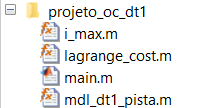
\includegraphics[]{Metodologia/Figuras/matlab_files.png}
    \label{fig:matlab_files}
    \caption*{\footnotesize{Fonte: Elaborada pelo autor.}}
\end{figure}


Durante a escrita do arquivo \lstinline[style=Matlab-editor]{main.m} uma dificuldade encontrada foi a determinação da variável \lstinline[style=Matlab-editor]{scale}, 
última  variável nos construtores \lstinline[style=Matlab-editor]{falcon.State()}, \lstinline[style=Matlab-editor]{falcon.Control()} e \lstinline[style=Matlab-editor]{falcon.Parameter()}.
Inicialmente os valores definidos foram a ordem de grandeza da cada variável o que gerou matrizes mau condicionadas no NLP e consequente um alto tempo de solução o problema. 
Os valores corretos, conforme sugerido no manual do FALCON.m\cite{manual:Falcon}, dever ser definidos de tal forma que a ordem de grandeza da variável seja um. Por exemplo: uma variávelque
representa a correte elétrica de um circuito em [mA] deve ter o parâmero \lstinline[style=Matlab-editor]{scale} igual a $10^{-3}$. 
A definição dos estados, variável de controle e parâmetros com o parâmetro \lstinline[style=Matlab-editor]{scale} adequado é apresentado no Código \ref{lst:scale}. 

\begin{figure}[h]
    \begin{lstlisting}[
        caption={[Trecho do arquivo main.m]Trecho do arquivo \lstinline[style=Matlab-editor]{main.m} com definição dos estados, variável de controle e parâmetros do OCP proposto}, 
        label={lst:scale},
        style      = Matlab-editor,
        basicstyle = \mlttfamily,
        firstnumber=4]
% vetor de estados
x_vec = [ falcon.State('x',   0,  11000, 1e-4);...
          falcon.State('v',   0,  12.5, 1e-1) ];
% variavel de controle
u_vec = falcon.Control('i', 0,  63, 1);
% tempo final
tf = falcon.Parameter('FinalTime', 1400, 0, 1400, 1e-3);
% raio do cilindro no motor
rm = falcon.Parameter('raioM', 0.026, 0.020, 0.050, 1e2);
    \end{lstlisting}
    \caption*{\footnotesize{Fonte: Elaborado pelo autor.}}
\end{figure}

Além disso, foi verificado que, a biblioteca FALCON.m versão v1.26 não funcionou no MATLAB  R2020a quando o optimizador  IPOPT era utilizado.
Isto ocorreu pois não há garantia de compatibilidade, no Windows, por parte do MATLAB  em sua evolução, a arquivos MEX (interface com programas escritos em C, C++ ou Fortran) gerados em versões 
anteriores e a biblioteca IPOPT é chamada por meio de um arquivo MEX não compatível apos a versão R2019b do MATLAB . Novas versões da FALCON.m
devem possibilitar o uso e versões mais novas do MATLAB  pois os arquivos MEX serão compilados novamente.




\clearpage
\chapter{Resultados}
\label{chap:resultados}

Os resultados obtidos com o desenvolvimento desse projeto são apresentados e discutidos nesse capitulo em três seções. 
Na Seção \ref{sec:resultados_modelo} 
A Seção \ref{sec:resultados_pista}
E a Seção \ref{sec:resultados_otimo}

\section{Modelo do veiculo DT1}
\label{sec:resultados_modelo}

O modelo obtido para o veiculo para o veiculo DT1 foi a Equação (\ref{eq:modelo_1}) e o conjunto de constates da Tabela \ref{tab:constantes}.
Entretanto esse modelo não foi validado experimentalmente pois esse projeto foi realizado, em sua maior parte, durante o regime de ensino remoto
emergência causado pela pandemia de Covid-19 em 2020. Na solução do OPC proposto a marca de consumo calculado para a estrategia ótima
foi de $900,3$ [km/kWh] que é um valor muito distante das marcas realmente realizas pelo DT1 de $266,5$ [km/kWh] em 2018 e de $226,9$ [km/kWh] em 2019  no Kartódromo de Sonoma na Shell Eco-marathon Americas. 
Apesar de que uma melhora na marca era esperada, esta grande diferença entre os valores das marcas deve ser analisada com ceticismo, ela indica que as constantes do modelo podem precisar ser ajustadas e/ou as simplificações revistas.


\section{Modelo da pista}
\label{sec:resultados_pista}

A curva ajustada para representar a altitude relativa em função da distancia apresentou um erro maior nos pontos que a distancia percorrida esta entre 290 e 575 e metros e entre 1005 e 1265 metros. O máximo erro destes
intervalos foi de 19\% e 34\% respetivamente. Ja no restante do intervalo o erro máximo ficou abaixo de 10\%. 
O modelo de inclinação, obtido a partir da arco tangente da derivada desta curva, foi aprestando na Equação (\ref{eq:modeloTheta}). 
A Figura \ref{graf:modelo_pista} apresenta uma comparação entre os dados de altitude e a curva ajusta.
O comportamento periódico desejado na curva ajustada para descrever a repetição das voltas na tentativa é a apresentado na \ref{graf:pista_voltas}.


\begin{figure}[H]
    \centering
    \caption{Curva ajustada para representar altitude da pista}
    % This file was created by matlab2tikz.
%
%The latest updates can be retrieved from
%  http://www.mathworks.com/matlabcentral/fileexchange/22022-matlab2tikz-matlab2tikz
%where you can also make suggestions and rate matlab2tikz.
%
\definecolor{mycolor1}{rgb}{0.00000,0.44700,0.74100}%
\definecolor{mycolor2}{rgb}{0.85000,0.32500,0.09800}%
%
\begin{tikzpicture}[scale=0.85]

\begin{axis}[%
width=4.521in,
height=3.566in,
at={(0.758in,0.481in)},
scale only axis,
xmin=0,
xmax=1440,
xlabel style={font=\color{white!15!black}},
xlabel={Distancia percorrida [m]},
ymin=-2,
ymax=5,
ylabel style={font=\color{white!15!black}},
ylabel={Altitude relativa [m]},
axis background/.style={fill=white},
xmajorgrids,
ymajorgrids,
legend style={legend cell align=left, align=left, draw=white!15!black}
]
\addplot [color=mycolor1, only marks, mark size=1.0pt, mark=o, mark options={solid, mycolor1}]
  table[row sep=crcr]{%
0	0\\
5.1222	0.035738\\
10.052	0.10497\\
15.102	0.10772\\
20.056	0.14341\\
25.018	0.18539\\
30.099	0.24281\\
35.019	0.26534\\
40.103	0.30621\\
45.03	0.34432\\
50.02	0.36324\\
55.06	0.4084\\
60.082	0.44874\\
65.003	0.50745\\
70.013	0.52866\\
75.043	0.54874\\
80.029	0.58008\\
85.054	0.60309\\
90.004	0.64756\\
95.034	0.69913\\
100.08	0.73437\\
105.09	0.77665\\
110.03	0.80147\\
115.11	0.8308\\
120.05	0.85947\\
125.08	0.91471\\
130.04	0.987\\
135.06	1.0446\\
140.02	1.1265\\
145.07	1.1976\\
150.07	1.2977\\
155.07	1.4261\\
160.05	1.5534\\
165.02	1.7003\\
170.06	1.8176\\
175.03	1.8384\\
180.1	1.8899\\
185.09	1.959\\
190.08	2.0057\\
195.07	2.0065\\
200.08	2.1076\\
205.05	2.2171\\
210.04	2.3643\\
215.1	2.5291\\
220.07	2.6873\\
225.1	2.8419\\
230.05	3.0317\\
235.08	3.1583\\
240.02	3.2784\\
245.01	3.4202\\
250.02	3.5219\\
255.05	3.6083\\
260.01	3.6875\\
265	3.8082\\
270.07	3.9549\\
275.02	4.0884\\
280.08	4.2276\\
285.07	4.3234\\
290.09	4.4291\\
295.02	4.4829\\
300.06	4.5449\\
305.07	4.61\\
310.07	4.648\\
315.05	4.6728\\
320.01	4.6917\\
325.05	4.7362\\
330.01	4.7312\\
335.08	4.7492\\
340.01	4.7603\\
345.05	4.7026\\
350.06	4.6628\\
355.04	4.5688\\
360.09	4.3908\\
365.05	4.1747\\
370.01	3.9563\\
375.05	3.7561\\
380.01	3.5984\\
385.01	3.5353\\
390.02	3.4615\\
395.07	3.4505\\
400.1	3.4657\\
405.04	3.5032\\
410.05	3.4511\\
415	3.3952\\
420.07	3.3656\\
425.01	3.2732\\
430.02	3.1978\\
435.03	3.1787\\
440.06	3.3637\\
445.07	3.6768\\
450.11	4.0237\\
455.11	4.3273\\
460.03	4.5621\\
465.01	4.7456\\
470.09	4.8381\\
475.01	4.8199\\
480.09	4.8295\\
485	4.8346\\
490.09	4.8057\\
495.09	4.7223\\
500.09	4.6332\\
505.1	4.5413\\
510.02	4.4621\\
515.05	4.3114\\
520.05	4.2162\\
525.01	4.134\\
530.04	4.0624\\
535.01	3.9909\\
540	3.9346\\
545.08	3.8595\\
550.12	3.8051\\
555.1	3.7335\\
560.09	3.6563\\
565.02	3.599\\
570.06	3.5572\\
575.09	3.5131\\
580.08	3.4391\\
585	3.3567\\
590.01	3.2757\\
595.05	3.2379\\
600.02	3.1674\\
605.08	3.0848\\
610.02	2.9922\\
615	2.9465\\
620.02	2.8593\\
625.11	2.7651\\
630.08	2.6997\\
635.08	2.6199\\
640.02	2.5204\\
645.04	2.4145\\
650.07	2.3246\\
655	2.2181\\
660.06	2.1146\\
665.02	2.038\\
670.06	1.9449\\
675.05	1.8925\\
680.09	1.8092\\
685.08	1.709\\
690.04	1.6652\\
695.04	1.5816\\
700.02	1.4836\\
705.1	1.4271\\
710.02	1.3237\\
715	1.2147\\
720.11	1.1747\\
725.08	1.0693\\
730.02	0.9783\\
735.02	0.87326\\
740.01	0.80079\\
745.06	0.67547\\
750.09	0.61633\\
755.06	0.53173\\
760.08	0.42591\\
765	0.38467\\
770.1	0.25097\\
775.04	0.185\\
780.1	0.094467\\
785.11	0.0042468\\
790.01	-0.087749\\
795.03	-0.15127\\
800.04	-0.19791\\
805.06	-0.29861\\
810.07	-0.35415\\
815.01	-0.43642\\
820.07	-0.50071\\
825.05	-0.5167\\
830.08	-0.56259\\
835.08	-0.6105\\
840.01	-0.64431\\
845.08	-0.66497\\
850.11	-0.67766\\
855.07	-0.70386\\
860.02	-0.69959\\
865.1	-0.70008\\
870.02	-0.72612\\
875.09	-0.75503\\
880.11	-0.74512\\
885.04	-0.72702\\
890.06	-0.72219\\
895.01	-0.74177\\
900.04	-0.74645\\
905.09	-0.78183\\
910.06	-0.79228\\
915.01	-0.79059\\
920.11	-0.80498\\
925	-0.81388\\
930.09	-0.82108\\
935.08	-0.85434\\
940.08	-0.87037\\
945.02	-0.8898\\
950.11	-0.91711\\
955	-0.941\\
960.02	-0.95908\\
965.01	-0.97259\\
970.07	-0.9977\\
975.02	-1.0021\\
980.02	-1.0205\\
985.06	-1.03\\
990.07	-1.0475\\
995.09	-1.0488\\
1000.1	-1.0607\\
1005	-1.0603\\
1010.1	-1.0762\\
1015	-1.0899\\
1020.1	-1.0865\\
1025	-1.1233\\
1030	-1.1057\\
1035.1	-1.1309\\
1040.1	-1.1516\\
1045.1	-1.1333\\
1050.1	-1.1306\\
1055	-1.1343\\
1060.1	-1.1496\\
1065	-1.2185\\
1070.1	-1.294\\
1075.1	-1.3496\\
1080.1	-1.4133\\
1085.1	-1.4789\\
1090.1	-1.4778\\
1095.1	-1.4619\\
1100	-1.4065\\
1105	-1.3362\\
1110.1	-1.2712\\
1115.1	-1.2374\\
1120.1	-1.1685\\
1125.1	-1.0986\\
1130	-1.0041\\
1135	-0.92332\\
1140	-0.88023\\
1145.1	-0.91493\\
1150.1	-0.9995\\
1155	-1.0491\\
1160.1	-1.1572\\
1165	-1.2352\\
1170.1	-1.2925\\
1175	-1.2543\\
1180.1	-1.2889\\
1185.1	-1.2424\\
1190.1	-1.2007\\
1195	-1.1524\\
1200.1	-1.0711\\
1205	-1.0818\\
1210	-1.0683\\
1215.1	-1.0743\\
1220	-1.0607\\
1225	-1.0466\\
1230.1	-1.0469\\
1235.1	-1.049\\
1240	-1.0506\\
1245	-1.0674\\
1250	-1.0704\\
1255.1	-1.0248\\
1260.1	-1.0326\\
1265	-1.0105\\
1270.1	-0.99422\\
1275	-0.98019\\
1280.1	-0.93839\\
1285	-0.93409\\
1290.1	-0.92035\\
1295.1	-0.9174\\
1300	-0.93492\\
1305.1	-0.91239\\
1310.1	-0.89661\\
1315.1	-0.85047\\
1320.1	-0.81659\\
1325.1	-0.76624\\
1330.1	-0.78241\\
1335	-0.77116\\
1340.1	-0.73442\\
1345.1	-0.71422\\
1350	-0.70423\\
1355	-0.66556\\
1360.1	-0.63987\\
1365.1	-0.60605\\
1370	-0.59789\\
1375	-0.54782\\
1380	-0.49583\\
1385	-0.46034\\
1390	-0.41838\\
1395.1	-0.363\\
1401.9	-0.32049\\
1406.3	-0.28726\\
1410.6	-0.25818\\
1415.1	-0.22964\\
1420	-0.17512\\
1425	-0.12472\\
1430.1	-0.10287\\
1435.1	-0.048184\\
1440	-0.01308\\
1440	0\\
1445.1222	0.035738\\
1450.052	0.10497\\
1455.102	0.10772\\
1460.056	0.14341\\
1465.018	0.18539\\
1470.099	0.24281\\
1475.019	0.26534\\
1480.103	0.30621\\
1485.03	0.34432\\
1490.02	0.36324\\
1495.06	0.4084\\
1500.082	0.44874\\
1505.003	0.50745\\
1510.013	0.52866\\
1515.043	0.54874\\
1520.029	0.58008\\
1525.054	0.60309\\
1530.004	0.64756\\
1535.034	0.69913\\
1540.08	0.73437\\
1545.09	0.77665\\
1550.03	0.80147\\
1555.11	0.8308\\
1560.05	0.85947\\
1565.08	0.91471\\
1570.04	0.987\\
1575.06	1.0446\\
1580.02	1.1265\\
1585.07	1.1976\\
1590.07	1.2977\\
1595.07	1.4261\\
1600.05	1.5534\\
1605.02	1.7003\\
1610.06	1.8176\\
1615.03	1.8384\\
1620.1	1.8899\\
1625.09	1.959\\
1630.08	2.0057\\
1635.07	2.0065\\
1640.08	2.1076\\
1645.05	2.2171\\
1650.04	2.3643\\
1655.1	2.5291\\
1660.07	2.6873\\
1665.1	2.8419\\
1670.05	3.0317\\
1675.08	3.1583\\
1680.02	3.2784\\
1685.01	3.4202\\
1690.02	3.5219\\
1695.05	3.6083\\
1700.01	3.6875\\
1705	3.8082\\
1710.07	3.9549\\
1715.02	4.0884\\
1720.08	4.2276\\
1725.07	4.3234\\
1730.09	4.4291\\
1735.02	4.4829\\
1740.06	4.5449\\
1745.07	4.61\\
1750.07	4.648\\
1755.05	4.6728\\
1760.01	4.6917\\
1765.05	4.7362\\
1770.01	4.7312\\
1775.08	4.7492\\
1780.01	4.7603\\
1785.05	4.7026\\
1790.06	4.6628\\
1795.04	4.5688\\
1800.09	4.3908\\
1805.05	4.1747\\
1810.01	3.9563\\
1815.05	3.7561\\
1820.01	3.5984\\
1825.01	3.5353\\
1830.02	3.4615\\
1835.07	3.4505\\
1840.1	3.4657\\
1845.04	3.5032\\
1850.05	3.4511\\
1855	3.3952\\
1860.07	3.3656\\
1865.01	3.2732\\
1870.02	3.1978\\
1875.03	3.1787\\
1880.06	3.3637\\
1885.07	3.6768\\
1890.11	4.0237\\
1895.11	4.3273\\
1900.03	4.5621\\
1905.01	4.7456\\
1910.09	4.8381\\
1915.01	4.8199\\
1920.09	4.8295\\
1925	4.8346\\
1930.09	4.8057\\
1935.09	4.7223\\
1940.09	4.6332\\
1945.1	4.5413\\
1950.02	4.4621\\
1955.05	4.3114\\
1960.05	4.2162\\
1965.01	4.134\\
1970.04	4.0624\\
1975.01	3.9909\\
1980	3.9346\\
1985.08	3.8595\\
1990.12	3.8051\\
1995.1	3.7335\\
2000.09	3.6563\\
2005.02	3.599\\
2010.06	3.5572\\
2015.09	3.5131\\
2020.08	3.4391\\
2025	3.3567\\
2030.01	3.2757\\
2035.05	3.2379\\
2040.02	3.1674\\
2045.08	3.0848\\
2050.02	2.9922\\
2055	2.9465\\
2060.02	2.8593\\
2065.11	2.7651\\
2070.08	2.6997\\
2075.08	2.6199\\
2080.02	2.5204\\
2085.04	2.4145\\
2090.07	2.3246\\
2095	2.2181\\
2100.06	2.1146\\
2105.02	2.038\\
2110.06	1.9449\\
2115.05	1.8925\\
2120.09	1.8092\\
2125.08	1.709\\
2130.04	1.6652\\
2135.04	1.5816\\
2140.02	1.4836\\
2145.1	1.4271\\
2150.02	1.3237\\
2155	1.2147\\
2160.11	1.1747\\
2165.08	1.0693\\
2170.02	0.9783\\
2175.02	0.87326\\
2180.01	0.80079\\
2185.06	0.67547\\
2190.09	0.61633\\
2195.06	0.53173\\
2200.08	0.42591\\
2205	0.38467\\
2210.1	0.25097\\
2215.04	0.185\\
2220.1	0.094467\\
2225.11	0.0042468\\
2230.01	-0.087749\\
2235.03	-0.15127\\
2240.04	-0.19791\\
2245.06	-0.29861\\
2250.07	-0.35415\\
2255.01	-0.43642\\
2260.07	-0.50071\\
2265.05	-0.5167\\
2270.08	-0.56259\\
2275.08	-0.6105\\
2280.01	-0.64431\\
2285.08	-0.66497\\
2290.11	-0.67766\\
2295.07	-0.70386\\
2300.02	-0.69959\\
2305.1	-0.70008\\
2310.02	-0.72612\\
2315.09	-0.75503\\
2320.11	-0.74512\\
2325.04	-0.72702\\
2330.06	-0.72219\\
2335.01	-0.74177\\
2340.04	-0.74645\\
2345.09	-0.78183\\
2350.06	-0.79228\\
2355.01	-0.79059\\
2360.11	-0.80498\\
2365	-0.81388\\
2370.09	-0.82108\\
2375.08	-0.85434\\
2380.08	-0.87037\\
2385.02	-0.8898\\
2390.11	-0.91711\\
2395	-0.941\\
2400.02	-0.95908\\
2405.01	-0.97259\\
2410.07	-0.9977\\
2415.02	-1.0021\\
2420.02	-1.0205\\
2425.06	-1.03\\
2430.07	-1.0475\\
2435.09	-1.0488\\
2440.1	-1.0607\\
2445	-1.0603\\
2450.1	-1.0762\\
2455	-1.0899\\
2460.1	-1.0865\\
2465	-1.1233\\
2470	-1.1057\\
2475.1	-1.1309\\
2480.1	-1.1516\\
2485.1	-1.1333\\
2490.1	-1.1306\\
2495	-1.1343\\
2500.1	-1.1496\\
2505	-1.2185\\
2510.1	-1.294\\
2515.1	-1.3496\\
2520.1	-1.4133\\
2525.1	-1.4789\\
2530.1	-1.4778\\
2535.1	-1.4619\\
2540	-1.4065\\
2545	-1.3362\\
2550.1	-1.2712\\
2555.1	-1.2374\\
2560.1	-1.1685\\
2565.1	-1.0986\\
2570	-1.0041\\
2575	-0.92332\\
2580	-0.88023\\
2585.1	-0.91493\\
2590.1	-0.9995\\
2595	-1.0491\\
2600.1	-1.1572\\
2605	-1.2352\\
2610.1	-1.2925\\
2615	-1.2543\\
2620.1	-1.2889\\
2625.1	-1.2424\\
2630.1	-1.2007\\
2635	-1.1524\\
2640.1	-1.0711\\
2645	-1.0818\\
2650	-1.0683\\
2655.1	-1.0743\\
2660	-1.0607\\
2665	-1.0466\\
2670.1	-1.0469\\
2675.1	-1.049\\
2680	-1.0506\\
2685	-1.0674\\
2690	-1.0704\\
2695.1	-1.0248\\
2700.1	-1.0326\\
2705	-1.0105\\
2710.1	-0.99422\\
2715	-0.98019\\
2720.1	-0.93839\\
2725	-0.93409\\
2730.1	-0.92035\\
2735.1	-0.9174\\
2740	-0.93492\\
2745.1	-0.91239\\
2750.1	-0.89661\\
2755.1	-0.85047\\
2760.1	-0.81659\\
2765.1	-0.76624\\
2770.1	-0.78241\\
2775	-0.77116\\
2780.1	-0.73442\\
2785.1	-0.71422\\
2790	-0.70423\\
2795	-0.66556\\
2800.1	-0.63987\\
2805.1	-0.60605\\
2810	-0.59789\\
2815	-0.54782\\
2820	-0.49583\\
2825	-0.46034\\
2830	-0.41838\\
2835.1	-0.363\\
2841.9	-0.32049\\
2846.3	-0.28726\\
2850.6	-0.25818\\
2855.1	-0.22964\\
2860	-0.17512\\
2865	-0.12472\\
2870.1	-0.10287\\
2875.1	-0.048184\\
2880	-0.01308\\
2880	0\\
2885.1222	0.035738\\
2890.052	0.10497\\
2895.102	0.10772\\
2900.056	0.14341\\
2905.018	0.18539\\
2910.099	0.24281\\
2915.019	0.26534\\
2920.103	0.30621\\
2925.03	0.34432\\
2930.02	0.36324\\
2935.06	0.4084\\
2940.082	0.44874\\
2945.003	0.50745\\
2950.013	0.52866\\
2955.043	0.54874\\
2960.029	0.58008\\
2965.054	0.60309\\
2970.004	0.64756\\
2975.034	0.69913\\
2980.08	0.73437\\
2985.09	0.77665\\
2990.03	0.80147\\
2995.11	0.8308\\
3000.05	0.85947\\
3005.08	0.91471\\
3010.04	0.987\\
3015.06	1.0446\\
3020.02	1.1265\\
3025.07	1.1976\\
3030.07	1.2977\\
3035.07	1.4261\\
3040.05	1.5534\\
3045.02	1.7003\\
3050.06	1.8176\\
3055.03	1.8384\\
3060.1	1.8899\\
3065.09	1.959\\
3070.08	2.0057\\
3075.07	2.0065\\
3080.08	2.1076\\
3085.05	2.2171\\
3090.04	2.3643\\
3095.1	2.5291\\
3100.07	2.6873\\
3105.1	2.8419\\
3110.05	3.0317\\
3115.08	3.1583\\
3120.02	3.2784\\
3125.01	3.4202\\
3130.02	3.5219\\
3135.05	3.6083\\
3140.01	3.6875\\
3145	3.8082\\
3150.07	3.9549\\
3155.02	4.0884\\
3160.08	4.2276\\
3165.07	4.3234\\
3170.09	4.4291\\
3175.02	4.4829\\
3180.06	4.5449\\
3185.07	4.61\\
3190.07	4.648\\
3195.05	4.6728\\
3200.01	4.6917\\
3205.05	4.7362\\
3210.01	4.7312\\
3215.08	4.7492\\
3220.01	4.7603\\
3225.05	4.7026\\
3230.06	4.6628\\
3235.04	4.5688\\
3240.09	4.3908\\
3245.05	4.1747\\
3250.01	3.9563\\
3255.05	3.7561\\
3260.01	3.5984\\
3265.01	3.5353\\
3270.02	3.4615\\
3275.07	3.4505\\
3280.1	3.4657\\
3285.04	3.5032\\
3290.05	3.4511\\
3295	3.3952\\
3300.07	3.3656\\
3305.01	3.2732\\
3310.02	3.1978\\
3315.03	3.1787\\
3320.06	3.3637\\
3325.07	3.6768\\
3330.11	4.0237\\
3335.11	4.3273\\
3340.03	4.5621\\
3345.01	4.7456\\
3350.09	4.8381\\
3355.01	4.8199\\
3360.09	4.8295\\
3365	4.8346\\
3370.09	4.8057\\
3375.09	4.7223\\
3380.09	4.6332\\
3385.1	4.5413\\
3390.02	4.4621\\
3395.05	4.3114\\
3400.05	4.2162\\
3405.01	4.134\\
3410.04	4.0624\\
3415.01	3.9909\\
3420	3.9346\\
3425.08	3.8595\\
3430.12	3.8051\\
3435.1	3.7335\\
3440.09	3.6563\\
3445.02	3.599\\
3450.06	3.5572\\
3455.09	3.5131\\
3460.08	3.4391\\
3465	3.3567\\
3470.01	3.2757\\
3475.05	3.2379\\
3480.02	3.1674\\
3485.08	3.0848\\
3490.02	2.9922\\
3495	2.9465\\
3500.02	2.8593\\
3505.11	2.7651\\
3510.08	2.6997\\
3515.08	2.6199\\
3520.02	2.5204\\
3525.04	2.4145\\
3530.07	2.3246\\
3535	2.2181\\
3540.06	2.1146\\
3545.02	2.038\\
3550.06	1.9449\\
3555.05	1.8925\\
3560.09	1.8092\\
3565.08	1.709\\
3570.04	1.6652\\
3575.04	1.5816\\
3580.02	1.4836\\
3585.1	1.4271\\
3590.02	1.3237\\
3595	1.2147\\
3600.11	1.1747\\
3605.08	1.0693\\
3610.02	0.9783\\
3615.02	0.87326\\
3620.01	0.80079\\
3625.06	0.67547\\
3630.09	0.61633\\
3635.06	0.53173\\
3640.08	0.42591\\
3645	0.38467\\
3650.1	0.25097\\
3655.04	0.185\\
3660.1	0.094467\\
3665.11	0.0042468\\
3670.01	-0.087749\\
3675.03	-0.15127\\
3680.04	-0.19791\\
3685.06	-0.29861\\
3690.07	-0.35415\\
3695.01	-0.43642\\
3700.07	-0.50071\\
3705.05	-0.5167\\
3710.08	-0.56259\\
3715.08	-0.6105\\
3720.01	-0.64431\\
3725.08	-0.66497\\
3730.11	-0.67766\\
3735.07	-0.70386\\
3740.02	-0.69959\\
3745.1	-0.70008\\
3750.02	-0.72612\\
3755.09	-0.75503\\
3760.11	-0.74512\\
3765.04	-0.72702\\
3770.06	-0.72219\\
3775.01	-0.74177\\
3780.04	-0.74645\\
3785.09	-0.78183\\
3790.06	-0.79228\\
3795.01	-0.79059\\
3800.11	-0.80498\\
3805	-0.81388\\
3810.09	-0.82108\\
3815.08	-0.85434\\
3820.08	-0.87037\\
3825.02	-0.8898\\
3830.11	-0.91711\\
3835	-0.941\\
3840.02	-0.95908\\
3845.01	-0.97259\\
3850.07	-0.9977\\
3855.02	-1.0021\\
3860.02	-1.0205\\
3865.06	-1.03\\
3870.07	-1.0475\\
3875.09	-1.0488\\
3880.1	-1.0607\\
3885	-1.0603\\
3890.1	-1.0762\\
3895	-1.0899\\
3900.1	-1.0865\\
3905	-1.1233\\
3910	-1.1057\\
3915.1	-1.1309\\
3920.1	-1.1516\\
3925.1	-1.1333\\
3930.1	-1.1306\\
3935	-1.1343\\
3940.1	-1.1496\\
3945	-1.2185\\
3950.1	-1.294\\
3955.1	-1.3496\\
3960.1	-1.4133\\
3965.1	-1.4789\\
3970.1	-1.4778\\
3975.1	-1.4619\\
3980	-1.4065\\
3985	-1.3362\\
3990.1	-1.2712\\
3995.1	-1.2374\\
4000.1	-1.1685\\
4005.1	-1.0986\\
4010	-1.0041\\
4015	-0.92332\\
4020	-0.88023\\
4025.1	-0.91493\\
4030.1	-0.9995\\
4035	-1.0491\\
4040.1	-1.1572\\
4045	-1.2352\\
4050.1	-1.2925\\
4055	-1.2543\\
4060.1	-1.2889\\
4065.1	-1.2424\\
4070.1	-1.2007\\
4075	-1.1524\\
4080.1	-1.0711\\
4085	-1.0818\\
4090	-1.0683\\
4095.1	-1.0743\\
4100	-1.0607\\
4105	-1.0466\\
4110.1	-1.0469\\
4115.1	-1.049\\
4120	-1.0506\\
4125	-1.0674\\
4130	-1.0704\\
4135.1	-1.0248\\
4140.1	-1.0326\\
4145	-1.0105\\
4150.1	-0.99422\\
4155	-0.98019\\
4160.1	-0.93839\\
4165	-0.93409\\
4170.1	-0.92035\\
4175.1	-0.9174\\
4180	-0.93492\\
4185.1	-0.91239\\
4190.1	-0.89661\\
4195.1	-0.85047\\
4200.1	-0.81659\\
4205.1	-0.76624\\
4210.1	-0.78241\\
4215	-0.77116\\
4220.1	-0.73442\\
4225.1	-0.71422\\
4230	-0.70423\\
4235	-0.66556\\
4240.1	-0.63987\\
4245.1	-0.60605\\
4250	-0.59789\\
4255	-0.54782\\
4260	-0.49583\\
4265	-0.46034\\
4270	-0.41838\\
4275.1	-0.363\\
4281.9	-0.32049\\
4286.3	-0.28726\\
4290.6	-0.25818\\
4295.1	-0.22964\\
4300	-0.17512\\
4305	-0.12472\\
4310.1	-0.10287\\
4315.1	-0.048184\\
4320	-0.01308\\
4320	0\\
4325.1222	0.035738\\
4330.052	0.10497\\
4335.102	0.10772\\
4340.056	0.14341\\
4345.018	0.18539\\
4350.099	0.24281\\
4355.019	0.26534\\
4360.103	0.30621\\
4365.03	0.34432\\
4370.02	0.36324\\
4375.06	0.4084\\
4380.082	0.44874\\
4385.003	0.50745\\
4390.013	0.52866\\
4395.043	0.54874\\
4400.029	0.58008\\
4405.054	0.60309\\
4410.004	0.64756\\
4415.034	0.69913\\
4420.08	0.73437\\
4425.09	0.77665\\
4430.03	0.80147\\
4435.11	0.8308\\
4440.05	0.85947\\
4445.08	0.91471\\
4450.04	0.987\\
4455.06	1.0446\\
4460.02	1.1265\\
4465.07	1.1976\\
4470.07	1.2977\\
4475.07	1.4261\\
4480.05	1.5534\\
4485.02	1.7003\\
4490.06	1.8176\\
4495.03	1.8384\\
4500.1	1.8899\\
4505.09	1.959\\
4510.08	2.0057\\
4515.07	2.0065\\
4520.08	2.1076\\
4525.05	2.2171\\
4530.04	2.3643\\
4535.1	2.5291\\
4540.07	2.6873\\
4545.1	2.8419\\
4550.05	3.0317\\
4555.08	3.1583\\
4560.02	3.2784\\
4565.01	3.4202\\
4570.02	3.5219\\
4575.05	3.6083\\
4580.01	3.6875\\
4585	3.8082\\
4590.07	3.9549\\
4595.02	4.0884\\
4600.08	4.2276\\
4605.07	4.3234\\
4610.09	4.4291\\
4615.02	4.4829\\
4620.06	4.5449\\
4625.07	4.61\\
4630.07	4.648\\
4635.05	4.6728\\
4640.01	4.6917\\
4645.05	4.7362\\
4650.01	4.7312\\
4655.08	4.7492\\
4660.01	4.7603\\
4665.05	4.7026\\
4670.06	4.6628\\
4675.04	4.5688\\
4680.09	4.3908\\
4685.05	4.1747\\
4690.01	3.9563\\
4695.05	3.7561\\
4700.01	3.5984\\
4705.01	3.5353\\
4710.02	3.4615\\
4715.07	3.4505\\
4720.1	3.4657\\
4725.04	3.5032\\
4730.05	3.4511\\
4735	3.3952\\
4740.07	3.3656\\
4745.01	3.2732\\
4750.02	3.1978\\
4755.03	3.1787\\
4760.06	3.3637\\
4765.07	3.6768\\
4770.11	4.0237\\
4775.11	4.3273\\
4780.03	4.5621\\
4785.01	4.7456\\
4790.09	4.8381\\
4795.01	4.8199\\
4800.09	4.8295\\
4805	4.8346\\
4810.09	4.8057\\
4815.09	4.7223\\
4820.09	4.6332\\
4825.1	4.5413\\
4830.02	4.4621\\
4835.05	4.3114\\
4840.05	4.2162\\
4845.01	4.134\\
4850.04	4.0624\\
4855.01	3.9909\\
4860	3.9346\\
4865.08	3.8595\\
4870.12	3.8051\\
4875.1	3.7335\\
4880.09	3.6563\\
4885.02	3.599\\
4890.06	3.5572\\
4895.09	3.5131\\
4900.08	3.4391\\
4905	3.3567\\
4910.01	3.2757\\
4915.05	3.2379\\
4920.02	3.1674\\
4925.08	3.0848\\
4930.02	2.9922\\
4935	2.9465\\
4940.02	2.8593\\
4945.11	2.7651\\
4950.08	2.6997\\
4955.08	2.6199\\
4960.02	2.5204\\
4965.04	2.4145\\
4970.07	2.3246\\
4975	2.2181\\
4980.06	2.1146\\
4985.02	2.038\\
4990.06	1.9449\\
4995.05	1.8925\\
5000.09	1.8092\\
5005.08	1.709\\
5010.04	1.6652\\
5015.04	1.5816\\
5020.02	1.4836\\
5025.1	1.4271\\
5030.02	1.3237\\
5035	1.2147\\
5040.11	1.1747\\
5045.08	1.0693\\
5050.02	0.9783\\
5055.02	0.87326\\
5060.01	0.80079\\
5065.06	0.67547\\
5070.09	0.61633\\
5075.06	0.53173\\
5080.08	0.42591\\
5085	0.38467\\
5090.1	0.25097\\
5095.04	0.185\\
5100.1	0.094467\\
5105.11	0.0042468\\
5110.01	-0.087749\\
5115.03	-0.15127\\
5120.04	-0.19791\\
5125.06	-0.29861\\
5130.07	-0.35415\\
5135.01	-0.43642\\
5140.07	-0.50071\\
5145.05	-0.5167\\
5150.08	-0.56259\\
5155.08	-0.6105\\
5160.01	-0.64431\\
5165.08	-0.66497\\
5170.11	-0.67766\\
5175.07	-0.70386\\
5180.02	-0.69959\\
5185.1	-0.70008\\
5190.02	-0.72612\\
5195.09	-0.75503\\
5200.11	-0.74512\\
5205.04	-0.72702\\
5210.06	-0.72219\\
5215.01	-0.74177\\
5220.04	-0.74645\\
5225.09	-0.78183\\
5230.06	-0.79228\\
5235.01	-0.79059\\
5240.11	-0.80498\\
5245	-0.81388\\
5250.09	-0.82108\\
5255.08	-0.85434\\
5260.08	-0.87037\\
5265.02	-0.8898\\
5270.11	-0.91711\\
5275	-0.941\\
5280.02	-0.95908\\
5285.01	-0.97259\\
5290.07	-0.9977\\
5295.02	-1.0021\\
5300.02	-1.0205\\
5305.06	-1.03\\
5310.07	-1.0475\\
5315.09	-1.0488\\
5320.1	-1.0607\\
5325	-1.0603\\
5330.1	-1.0762\\
5335	-1.0899\\
5340.1	-1.0865\\
5345	-1.1233\\
5350	-1.1057\\
5355.1	-1.1309\\
5360.1	-1.1516\\
5365.1	-1.1333\\
5370.1	-1.1306\\
5375	-1.1343\\
5380.1	-1.1496\\
5385	-1.2185\\
5390.1	-1.294\\
5395.1	-1.3496\\
5400.1	-1.4133\\
5405.1	-1.4789\\
5410.1	-1.4778\\
5415.1	-1.4619\\
5420	-1.4065\\
5425	-1.3362\\
5430.1	-1.2712\\
5435.1	-1.2374\\
5440.1	-1.1685\\
5445.1	-1.0986\\
5450	-1.0041\\
5455	-0.92332\\
5460	-0.88023\\
5465.1	-0.91493\\
5470.1	-0.9995\\
5475	-1.0491\\
5480.1	-1.1572\\
5485	-1.2352\\
5490.1	-1.2925\\
5495	-1.2543\\
5500.1	-1.2889\\
5505.1	-1.2424\\
5510.1	-1.2007\\
5515	-1.1524\\
5520.1	-1.0711\\
5525	-1.0818\\
5530	-1.0683\\
5535.1	-1.0743\\
5540	-1.0607\\
5545	-1.0466\\
5550.1	-1.0469\\
5555.1	-1.049\\
5560	-1.0506\\
5565	-1.0674\\
5570	-1.0704\\
5575.1	-1.0248\\
5580.1	-1.0326\\
5585	-1.0105\\
5590.1	-0.99422\\
5595	-0.98019\\
5600.1	-0.93839\\
5605	-0.93409\\
5610.1	-0.92035\\
5615.1	-0.9174\\
5620	-0.93492\\
5625.1	-0.91239\\
5630.1	-0.89661\\
5635.1	-0.85047\\
5640.1	-0.81659\\
5645.1	-0.76624\\
5650.1	-0.78241\\
5655	-0.77116\\
5660.1	-0.73442\\
5665.1	-0.71422\\
5670	-0.70423\\
5675	-0.66556\\
5680.1	-0.63987\\
5685.1	-0.60605\\
5690	-0.59789\\
5695	-0.54782\\
5700	-0.49583\\
5705	-0.46034\\
5710	-0.41838\\
5715.1	-0.363\\
5721.9	-0.32049\\
5726.3	-0.28726\\
5730.6	-0.25818\\
5735.1	-0.22964\\
5740	-0.17512\\
5745	-0.12472\\
5750.1	-0.10287\\
5755.1	-0.048184\\
5760	-0.01308\\
5760	0\\
5765.1222	0.035738\\
5770.052	0.10497\\
5775.102	0.10772\\
5780.056	0.14341\\
5785.018	0.18539\\
5790.099	0.24281\\
5795.019	0.26534\\
5800.103	0.30621\\
5805.03	0.34432\\
5810.02	0.36324\\
5815.06	0.4084\\
5820.082	0.44874\\
5825.003	0.50745\\
5830.013	0.52866\\
5835.043	0.54874\\
5840.029	0.58008\\
5845.054	0.60309\\
5850.004	0.64756\\
5855.034	0.69913\\
5860.08	0.73437\\
5865.09	0.77665\\
5870.03	0.80147\\
5875.11	0.8308\\
5880.05	0.85947\\
5885.08	0.91471\\
5890.04	0.987\\
5895.06	1.0446\\
5900.02	1.1265\\
5905.07	1.1976\\
5910.07	1.2977\\
5915.07	1.4261\\
5920.05	1.5534\\
5925.02	1.7003\\
5930.06	1.8176\\
5935.03	1.8384\\
5940.1	1.8899\\
5945.09	1.959\\
5950.08	2.0057\\
5955.07	2.0065\\
5960.08	2.1076\\
5965.05	2.2171\\
5970.04	2.3643\\
5975.1	2.5291\\
5980.07	2.6873\\
5985.1	2.8419\\
5990.05	3.0317\\
5995.08	3.1583\\
6000.02	3.2784\\
6005.01	3.4202\\
6010.02	3.5219\\
6015.05	3.6083\\
6020.01	3.6875\\
6025	3.8082\\
6030.07	3.9549\\
6035.02	4.0884\\
6040.08	4.2276\\
6045.07	4.3234\\
6050.09	4.4291\\
6055.02	4.4829\\
6060.06	4.5449\\
6065.07	4.61\\
6070.07	4.648\\
6075.05	4.6728\\
6080.01	4.6917\\
6085.05	4.7362\\
6090.01	4.7312\\
6095.08	4.7492\\
6100.01	4.7603\\
6105.05	4.7026\\
6110.06	4.6628\\
6115.04	4.5688\\
6120.09	4.3908\\
6125.05	4.1747\\
6130.01	3.9563\\
6135.05	3.7561\\
6140.01	3.5984\\
6145.01	3.5353\\
6150.02	3.4615\\
6155.07	3.4505\\
6160.1	3.4657\\
6165.04	3.5032\\
6170.05	3.4511\\
6175	3.3952\\
6180.07	3.3656\\
6185.01	3.2732\\
6190.02	3.1978\\
6195.03	3.1787\\
6200.06	3.3637\\
6205.07	3.6768\\
6210.11	4.0237\\
6215.11	4.3273\\
6220.03	4.5621\\
6225.01	4.7456\\
6230.09	4.8381\\
6235.01	4.8199\\
6240.09	4.8295\\
6245	4.8346\\
6250.09	4.8057\\
6255.09	4.7223\\
6260.09	4.6332\\
6265.1	4.5413\\
6270.02	4.4621\\
6275.05	4.3114\\
6280.05	4.2162\\
6285.01	4.134\\
6290.04	4.0624\\
6295.01	3.9909\\
6300	3.9346\\
6305.08	3.8595\\
6310.12	3.8051\\
6315.1	3.7335\\
6320.09	3.6563\\
6325.02	3.599\\
6330.06	3.5572\\
6335.09	3.5131\\
6340.08	3.4391\\
6345	3.3567\\
6350.01	3.2757\\
6355.05	3.2379\\
6360.02	3.1674\\
6365.08	3.0848\\
6370.02	2.9922\\
6375	2.9465\\
6380.02	2.8593\\
6385.11	2.7651\\
6390.08	2.6997\\
6395.08	2.6199\\
6400.02	2.5204\\
6405.04	2.4145\\
6410.07	2.3246\\
6415	2.2181\\
6420.06	2.1146\\
6425.02	2.038\\
6430.06	1.9449\\
6435.05	1.8925\\
6440.09	1.8092\\
6445.08	1.709\\
6450.04	1.6652\\
6455.04	1.5816\\
6460.02	1.4836\\
6465.1	1.4271\\
6470.02	1.3237\\
6475	1.2147\\
6480.11	1.1747\\
6485.08	1.0693\\
6490.02	0.9783\\
6495.02	0.87326\\
6500.01	0.80079\\
6505.06	0.67547\\
6510.09	0.61633\\
6515.06	0.53173\\
6520.08	0.42591\\
6525	0.38467\\
6530.1	0.25097\\
6535.04	0.185\\
6540.1	0.094467\\
6545.11	0.0042468\\
6550.01	-0.087749\\
6555.03	-0.15127\\
6560.04	-0.19791\\
6565.06	-0.29861\\
6570.07	-0.35415\\
6575.01	-0.43642\\
6580.07	-0.50071\\
6585.05	-0.5167\\
6590.08	-0.56259\\
6595.08	-0.6105\\
6600.01	-0.64431\\
6605.08	-0.66497\\
6610.11	-0.67766\\
6615.07	-0.70386\\
6620.02	-0.69959\\
6625.1	-0.70008\\
6630.02	-0.72612\\
6635.09	-0.75503\\
6640.11	-0.74512\\
6645.04	-0.72702\\
6650.06	-0.72219\\
6655.01	-0.74177\\
6660.04	-0.74645\\
6665.09	-0.78183\\
6670.06	-0.79228\\
6675.01	-0.79059\\
6680.11	-0.80498\\
6685	-0.81388\\
6690.09	-0.82108\\
6695.08	-0.85434\\
6700.08	-0.87037\\
6705.02	-0.8898\\
6710.11	-0.91711\\
6715	-0.941\\
6720.02	-0.95908\\
6725.01	-0.97259\\
6730.07	-0.9977\\
6735.02	-1.0021\\
6740.02	-1.0205\\
6745.06	-1.03\\
6750.07	-1.0475\\
6755.09	-1.0488\\
6760.1	-1.0607\\
6765	-1.0603\\
6770.1	-1.0762\\
6775	-1.0899\\
6780.1	-1.0865\\
6785	-1.1233\\
6790	-1.1057\\
6795.1	-1.1309\\
6800.1	-1.1516\\
6805.1	-1.1333\\
6810.1	-1.1306\\
6815	-1.1343\\
6820.1	-1.1496\\
6825	-1.2185\\
6830.1	-1.294\\
6835.1	-1.3496\\
6840.1	-1.4133\\
6845.1	-1.4789\\
6850.1	-1.4778\\
6855.1	-1.4619\\
6860	-1.4065\\
6865	-1.3362\\
6870.1	-1.2712\\
6875.1	-1.2374\\
6880.1	-1.1685\\
6885.1	-1.0986\\
6890	-1.0041\\
6895	-0.92332\\
6900	-0.88023\\
6905.1	-0.91493\\
6910.1	-0.9995\\
6915	-1.0491\\
6920.1	-1.1572\\
6925	-1.2352\\
6930.1	-1.2925\\
6935	-1.2543\\
6940.1	-1.2889\\
6945.1	-1.2424\\
6950.1	-1.2007\\
6955	-1.1524\\
6960.1	-1.0711\\
6965	-1.0818\\
6970	-1.0683\\
6975.1	-1.0743\\
6980	-1.0607\\
6985	-1.0466\\
6990.1	-1.0469\\
6995.1	-1.049\\
7000	-1.0506\\
7005	-1.0674\\
7010	-1.0704\\
7015.1	-1.0248\\
7020.1	-1.0326\\
7025	-1.0105\\
7030.1	-0.99422\\
7035	-0.98019\\
7040.1	-0.93839\\
7045	-0.93409\\
7050.1	-0.92035\\
7055.1	-0.9174\\
7060	-0.93492\\
7065.1	-0.91239\\
7070.1	-0.89661\\
7075.1	-0.85047\\
7080.1	-0.81659\\
7085.1	-0.76624\\
7090.1	-0.78241\\
7095	-0.77116\\
7100.1	-0.73442\\
7105.1	-0.71422\\
7110	-0.70423\\
7115	-0.66556\\
7120.1	-0.63987\\
7125.1	-0.60605\\
7130	-0.59789\\
7135	-0.54782\\
7140	-0.49583\\
7145	-0.46034\\
7150	-0.41838\\
7155.1	-0.363\\
7161.9	-0.32049\\
7166.3	-0.28726\\
7170.6	-0.25818\\
7175.1	-0.22964\\
7180	-0.17512\\
7185	-0.12472\\
7190.1	-0.10287\\
7195.1	-0.048184\\
7200	-0.01308\\
7200	0\\
7205.1222	0.035738\\
7210.052	0.10497\\
7215.102	0.10772\\
7220.056	0.14341\\
7225.018	0.18539\\
7230.099	0.24281\\
7235.019	0.26534\\
7240.103	0.30621\\
7245.03	0.34432\\
7250.02	0.36324\\
7255.06	0.4084\\
7260.082	0.44874\\
7265.003	0.50745\\
7270.013	0.52866\\
7275.043	0.54874\\
7280.029	0.58008\\
7285.054	0.60309\\
7290.004	0.64756\\
7295.034	0.69913\\
7300.08	0.73437\\
7305.09	0.77665\\
7310.03	0.80147\\
7315.11	0.8308\\
7320.05	0.85947\\
7325.08	0.91471\\
7330.04	0.987\\
7335.06	1.0446\\
7340.02	1.1265\\
7345.07	1.1976\\
7350.07	1.2977\\
7355.07	1.4261\\
7360.05	1.5534\\
7365.02	1.7003\\
7370.06	1.8176\\
7375.03	1.8384\\
7380.1	1.8899\\
7385.09	1.959\\
7390.08	2.0057\\
7395.07	2.0065\\
7400.08	2.1076\\
7405.05	2.2171\\
7410.04	2.3643\\
7415.1	2.5291\\
7420.07	2.6873\\
7425.1	2.8419\\
7430.05	3.0317\\
7435.08	3.1583\\
7440.02	3.2784\\
7445.01	3.4202\\
7450.02	3.5219\\
7455.05	3.6083\\
7460.01	3.6875\\
7465	3.8082\\
7470.07	3.9549\\
7475.02	4.0884\\
7480.08	4.2276\\
7485.07	4.3234\\
7490.09	4.4291\\
7495.02	4.4829\\
7500.06	4.5449\\
7505.07	4.61\\
7510.07	4.648\\
7515.05	4.6728\\
7520.01	4.6917\\
7525.05	4.7362\\
7530.01	4.7312\\
7535.08	4.7492\\
7540.01	4.7603\\
7545.05	4.7026\\
7550.06	4.6628\\
7555.04	4.5688\\
7560.09	4.3908\\
7565.05	4.1747\\
7570.01	3.9563\\
7575.05	3.7561\\
7580.01	3.5984\\
7585.01	3.5353\\
7590.02	3.4615\\
7595.07	3.4505\\
7600.1	3.4657\\
7605.04	3.5032\\
7610.05	3.4511\\
7615	3.3952\\
7620.07	3.3656\\
7625.01	3.2732\\
7630.02	3.1978\\
7635.03	3.1787\\
7640.06	3.3637\\
7645.07	3.6768\\
7650.11	4.0237\\
7655.11	4.3273\\
7660.03	4.5621\\
7665.01	4.7456\\
7670.09	4.8381\\
7675.01	4.8199\\
7680.09	4.8295\\
7685	4.8346\\
7690.09	4.8057\\
7695.09	4.7223\\
7700.09	4.6332\\
7705.1	4.5413\\
7710.02	4.4621\\
7715.05	4.3114\\
7720.05	4.2162\\
7725.01	4.134\\
7730.04	4.0624\\
7735.01	3.9909\\
7740	3.9346\\
7745.08	3.8595\\
7750.12	3.8051\\
7755.1	3.7335\\
7760.09	3.6563\\
7765.02	3.599\\
7770.06	3.5572\\
7775.09	3.5131\\
7780.08	3.4391\\
7785	3.3567\\
7790.01	3.2757\\
7795.05	3.2379\\
7800.02	3.1674\\
7805.08	3.0848\\
7810.02	2.9922\\
7815	2.9465\\
7820.02	2.8593\\
7825.11	2.7651\\
7830.08	2.6997\\
7835.08	2.6199\\
7840.02	2.5204\\
7845.04	2.4145\\
7850.07	2.3246\\
7855	2.2181\\
7860.06	2.1146\\
7865.02	2.038\\
7870.06	1.9449\\
7875.05	1.8925\\
7880.09	1.8092\\
7885.08	1.709\\
7890.04	1.6652\\
7895.04	1.5816\\
7900.02	1.4836\\
7905.1	1.4271\\
7910.02	1.3237\\
7915	1.2147\\
7920.11	1.1747\\
7925.08	1.0693\\
7930.02	0.9783\\
7935.02	0.87326\\
7940.01	0.80079\\
7945.06	0.67547\\
7950.09	0.61633\\
7955.06	0.53173\\
7960.08	0.42591\\
7965	0.38467\\
7970.1	0.25097\\
7975.04	0.185\\
7980.1	0.094467\\
7985.11	0.0042468\\
7990.01	-0.087749\\
7995.03	-0.15127\\
8000.04	-0.19791\\
8005.06	-0.29861\\
8010.07	-0.35415\\
8015.01	-0.43642\\
8020.07	-0.50071\\
8025.05	-0.5167\\
8030.08	-0.56259\\
8035.08	-0.6105\\
8040.01	-0.64431\\
8045.08	-0.66497\\
8050.11	-0.67766\\
8055.07	-0.70386\\
8060.02	-0.69959\\
8065.1	-0.70008\\
8070.02	-0.72612\\
8075.09	-0.75503\\
8080.11	-0.74512\\
8085.04	-0.72702\\
8090.06	-0.72219\\
8095.01	-0.74177\\
8100.04	-0.74645\\
8105.09	-0.78183\\
8110.06	-0.79228\\
8115.01	-0.79059\\
8120.11	-0.80498\\
8125	-0.81388\\
8130.09	-0.82108\\
8135.08	-0.85434\\
8140.08	-0.87037\\
8145.02	-0.8898\\
8150.11	-0.91711\\
8155	-0.941\\
8160.02	-0.95908\\
8165.01	-0.97259\\
8170.07	-0.9977\\
8175.02	-1.0021\\
8180.02	-1.0205\\
8185.06	-1.03\\
8190.07	-1.0475\\
8195.09	-1.0488\\
8200.1	-1.0607\\
8205	-1.0603\\
8210.1	-1.0762\\
8215	-1.0899\\
8220.1	-1.0865\\
8225	-1.1233\\
8230	-1.1057\\
8235.1	-1.1309\\
8240.1	-1.1516\\
8245.1	-1.1333\\
8250.1	-1.1306\\
8255	-1.1343\\
8260.1	-1.1496\\
8265	-1.2185\\
8270.1	-1.294\\
8275.1	-1.3496\\
8280.1	-1.4133\\
8285.1	-1.4789\\
8290.1	-1.4778\\
8295.1	-1.4619\\
8300	-1.4065\\
8305	-1.3362\\
8310.1	-1.2712\\
8315.1	-1.2374\\
8320.1	-1.1685\\
8325.1	-1.0986\\
8330	-1.0041\\
8335	-0.92332\\
8340	-0.88023\\
8345.1	-0.91493\\
8350.1	-0.9995\\
8355	-1.0491\\
8360.1	-1.1572\\
8365	-1.2352\\
8370.1	-1.2925\\
8375	-1.2543\\
8380.1	-1.2889\\
8385.1	-1.2424\\
8390.1	-1.2007\\
8395	-1.1524\\
8400.1	-1.0711\\
8405	-1.0818\\
8410	-1.0683\\
8415.1	-1.0743\\
8420	-1.0607\\
8425	-1.0466\\
8430.1	-1.0469\\
8435.1	-1.049\\
8440	-1.0506\\
8445	-1.0674\\
8450	-1.0704\\
8455.1	-1.0248\\
8460.1	-1.0326\\
8465	-1.0105\\
8470.1	-0.99422\\
8475	-0.98019\\
8480.1	-0.93839\\
8485	-0.93409\\
8490.1	-0.92035\\
8495.1	-0.9174\\
8500	-0.93492\\
8505.1	-0.91239\\
8510.1	-0.89661\\
8515.1	-0.85047\\
8520.1	-0.81659\\
8525.1	-0.76624\\
8530.1	-0.78241\\
8535	-0.77116\\
8540.1	-0.73442\\
8545.1	-0.71422\\
8550	-0.70423\\
8555	-0.66556\\
8560.1	-0.63987\\
8565.1	-0.60605\\
8570	-0.59789\\
8575	-0.54782\\
8580	-0.49583\\
8585	-0.46034\\
8590	-0.41838\\
8595.1	-0.363\\
8601.9	-0.32049\\
8606.3	-0.28726\\
8610.6	-0.25818\\
8615.1	-0.22964\\
8620	-0.17512\\
8625	-0.12472\\
8630.1	-0.10287\\
8635.1	-0.048184\\
8640	-0.01308\\
8640	0\\
8645.1222	0.035738\\
8650.052	0.10497\\
8655.102	0.10772\\
8660.056	0.14341\\
8665.018	0.18539\\
8670.099	0.24281\\
8675.019	0.26534\\
8680.103	0.30621\\
8685.03	0.34432\\
8690.02	0.36324\\
8695.06	0.4084\\
8700.082	0.44874\\
8705.003	0.50745\\
8710.013	0.52866\\
8715.043	0.54874\\
8720.029	0.58008\\
8725.054	0.60309\\
8730.004	0.64756\\
8735.034	0.69913\\
8740.08	0.73437\\
8745.09	0.77665\\
8750.03	0.80147\\
8755.11	0.8308\\
8760.05	0.85947\\
8765.08	0.91471\\
8770.04	0.987\\
8775.06	1.0446\\
8780.02	1.1265\\
8785.07	1.1976\\
8790.07	1.2977\\
8795.07	1.4261\\
8800.05	1.5534\\
8805.02	1.7003\\
8810.06	1.8176\\
8815.03	1.8384\\
8820.1	1.8899\\
8825.09	1.959\\
8830.08	2.0057\\
8835.07	2.0065\\
8840.08	2.1076\\
8845.05	2.2171\\
8850.04	2.3643\\
8855.1	2.5291\\
8860.07	2.6873\\
8865.1	2.8419\\
8870.05	3.0317\\
8875.08	3.1583\\
8880.02	3.2784\\
8885.01	3.4202\\
8890.02	3.5219\\
8895.05	3.6083\\
8900.01	3.6875\\
8905	3.8082\\
8910.07	3.9549\\
8915.02	4.0884\\
8920.08	4.2276\\
8925.07	4.3234\\
8930.09	4.4291\\
8935.02	4.4829\\
8940.06	4.5449\\
8945.07	4.61\\
8950.07	4.648\\
8955.05	4.6728\\
8960.01	4.6917\\
8965.05	4.7362\\
8970.01	4.7312\\
8975.08	4.7492\\
8980.01	4.7603\\
8985.05	4.7026\\
8990.06	4.6628\\
8995.04	4.5688\\
9000.09	4.3908\\
9005.05	4.1747\\
9010.01	3.9563\\
9015.05	3.7561\\
9020.01	3.5984\\
9025.01	3.5353\\
9030.02	3.4615\\
9035.07	3.4505\\
9040.1	3.4657\\
9045.04	3.5032\\
9050.05	3.4511\\
9055	3.3952\\
9060.07	3.3656\\
9065.01	3.2732\\
9070.02	3.1978\\
9075.03	3.1787\\
9080.06	3.3637\\
9085.07	3.6768\\
9090.11	4.0237\\
9095.11	4.3273\\
9100.03	4.5621\\
9105.01	4.7456\\
9110.09	4.8381\\
9115.01	4.8199\\
9120.09	4.8295\\
9125	4.8346\\
9130.09	4.8057\\
9135.09	4.7223\\
9140.09	4.6332\\
9145.1	4.5413\\
9150.02	4.4621\\
9155.05	4.3114\\
9160.05	4.2162\\
9165.01	4.134\\
9170.04	4.0624\\
9175.01	3.9909\\
9180	3.9346\\
9185.08	3.8595\\
9190.12	3.8051\\
9195.1	3.7335\\
9200.09	3.6563\\
9205.02	3.599\\
9210.06	3.5572\\
9215.09	3.5131\\
9220.08	3.4391\\
9225	3.3567\\
9230.01	3.2757\\
9235.05	3.2379\\
9240.02	3.1674\\
9245.08	3.0848\\
9250.02	2.9922\\
9255	2.9465\\
9260.02	2.8593\\
9265.11	2.7651\\
9270.08	2.6997\\
9275.08	2.6199\\
9280.02	2.5204\\
9285.04	2.4145\\
9290.07	2.3246\\
9295	2.2181\\
9300.06	2.1146\\
9305.02	2.038\\
9310.06	1.9449\\
9315.05	1.8925\\
9320.09	1.8092\\
9325.08	1.709\\
9330.04	1.6652\\
9335.04	1.5816\\
9340.02	1.4836\\
9345.1	1.4271\\
9350.02	1.3237\\
9355	1.2147\\
9360.11	1.1747\\
9365.08	1.0693\\
9370.02	0.9783\\
9375.02	0.87326\\
9380.01	0.80079\\
9385.06	0.67547\\
9390.09	0.61633\\
9395.06	0.53173\\
9400.08	0.42591\\
9405	0.38467\\
9410.1	0.25097\\
9415.04	0.185\\
9420.1	0.094467\\
9425.11	0.0042468\\
9430.01	-0.087749\\
9435.03	-0.15127\\
9440.04	-0.19791\\
9445.06	-0.29861\\
9450.07	-0.35415\\
9455.01	-0.43642\\
9460.07	-0.50071\\
9465.05	-0.5167\\
9470.08	-0.56259\\
9475.08	-0.6105\\
9480.01	-0.64431\\
9485.08	-0.66497\\
9490.11	-0.67766\\
9495.07	-0.70386\\
9500.02	-0.69959\\
9505.1	-0.70008\\
9510.02	-0.72612\\
9515.09	-0.75503\\
9520.11	-0.74512\\
9525.04	-0.72702\\
9530.06	-0.72219\\
9535.01	-0.74177\\
9540.04	-0.74645\\
9545.09	-0.78183\\
9550.06	-0.79228\\
9555.01	-0.79059\\
9560.11	-0.80498\\
9565	-0.81388\\
9570.09	-0.82108\\
9575.08	-0.85434\\
9580.08	-0.87037\\
9585.02	-0.8898\\
9590.11	-0.91711\\
9595	-0.941\\
9600.02	-0.95908\\
9605.01	-0.97259\\
9610.07	-0.9977\\
9615.02	-1.0021\\
9620.02	-1.0205\\
9625.06	-1.03\\
9630.07	-1.0475\\
9635.09	-1.0488\\
9640.1	-1.0607\\
9645	-1.0603\\
9650.1	-1.0762\\
9655	-1.0899\\
9660.1	-1.0865\\
9665	-1.1233\\
9670	-1.1057\\
9675.1	-1.1309\\
9680.1	-1.1516\\
9685.1	-1.1333\\
9690.1	-1.1306\\
9695	-1.1343\\
9700.1	-1.1496\\
9705	-1.2185\\
9710.1	-1.294\\
9715.1	-1.3496\\
9720.1	-1.4133\\
9725.1	-1.4789\\
9730.1	-1.4778\\
9735.1	-1.4619\\
9740	-1.4065\\
9745	-1.3362\\
9750.1	-1.2712\\
9755.1	-1.2374\\
9760.1	-1.1685\\
9765.1	-1.0986\\
9770	-1.0041\\
9775	-0.92332\\
9780	-0.88023\\
9785.1	-0.91493\\
9790.1	-0.9995\\
9795	-1.0491\\
9800.1	-1.1572\\
9805	-1.2352\\
9810.1	-1.2925\\
9815	-1.2543\\
9820.1	-1.2889\\
9825.1	-1.2424\\
9830.1	-1.2007\\
9835	-1.1524\\
9840.1	-1.0711\\
9845	-1.0818\\
9850	-1.0683\\
9855.1	-1.0743\\
9860	-1.0607\\
9865	-1.0466\\
9870.1	-1.0469\\
9875.1	-1.049\\
9880	-1.0506\\
9885	-1.0674\\
9890	-1.0704\\
9895.1	-1.0248\\
9900.1	-1.0326\\
9905	-1.0105\\
9910.1	-0.99422\\
9915	-0.98019\\
9920.1	-0.93839\\
9925	-0.93409\\
9930.1	-0.92035\\
9935.1	-0.9174\\
9940	-0.93492\\
9945.1	-0.91239\\
9950.1	-0.89661\\
9955.1	-0.85047\\
9960.1	-0.81659\\
9965.1	-0.76624\\
9970.1	-0.78241\\
9975	-0.77116\\
9980.1	-0.73442\\
9985.1	-0.71422\\
9990	-0.70423\\
9995	-0.66556\\
10000.1	-0.63987\\
10005.1	-0.60605\\
10010	-0.59789\\
10015	-0.54782\\
10020	-0.49583\\
10025	-0.46034\\
10030	-0.41838\\
10035.1	-0.363\\
10041.9	-0.32049\\
10046.3	-0.28726\\
10050.6	-0.25818\\
10055.1	-0.22964\\
10060	-0.17512\\
10065	-0.12472\\
10070.1	-0.10287\\
10075.1	-0.048184\\
10080	-0.01308\\
};
\addlegendentry{Dados}

\addplot [color=mycolor2, line width=2.0pt]
  table[row sep=crcr]{%
1	-0.109711917352081\\
2	-0.0997651899252466\\
3	-0.0897698810709357\\
4	-0.0797287446201807\\
5	-0.0696445893482892\\
6	-0.0595202761884084\\
7	-0.0493587153657857\\
8	-0.0391628634552307\\
9	-0.0289357203643766\\
10	-0.0186803262454241\\
11	-0.00839975833814072\\
12	0.00190287225302775\\
13	0.0122244238447967\\
14	0.0225617275208154\\
15	0.0329115905342793\\
16	0.0432707997642147\\
17	0.0536361252221968\\
18	0.0640043236061954\\
19	0.0743721418981765\\
20	0.0847363210020255\\
21	0.0950935994183011\\
22	0.10544071695227\\
23	0.115774418451625\\
24	0.126091457570232\\
25	0.136388600554215\\
26	0.146662630046643\\
27	0.156910348907032\\
28	0.167128584041869\\
29	0.177314190242296\\
30	0.187464054025096\\
31	0.197575097473076\\
32	0.207644282070944\\
33	0.217668612532733\\
34	0.227645140616833\\
35	0.237570968924681\\
36	0.247443254679135\\
37	0.257259213478585\\
38	0.267016123022827\\
39	0.276711326806761\\
40	0.286342237777955\\
41	0.295906341954157\\
42	0.305401201996829\\
43	0.31482446073683\\
44	0.324173844648373\\
45	0.333447167267411\\
46	0.342642332550677\\
47	0.351757338171582\\
48	0.360790278749266\\
49	0.369739349007116\\
50	0.378602846857121\\
51	0.387379176406482\\
52	0.396066850882955\\
53	0.404664495475469\\
54	0.413170850086601\\
55	0.421584771993597\\
56	0.429905238414653\\
57	0.438131348977282\\
58	0.446262328085635\\
59	0.454297527183765\\
60	0.462236426911864\\
61	0.470078639152616\\
62	0.477823908964901\\
63	0.48547211640215\\
64	0.493023278212789\\
65	0.500477549420268\\
66	0.507835224780295\\
67	0.515096740113001\\
68	0.522262673507857\\
69	0.529333746399276\\
70	0.536310824510952\\
71	0.543194918667103\\
72	0.549987185468885\\
73	0.556688927834383\\
74	0.563301595400693\\
75	0.569826784786738\\
76	0.576266239715584\\
77	0.582621850995138\\
78	0.588895656356266\\
79	0.595089840147451\\
80	0.601206732885304\\
81	0.607248810660309\\
82	0.613218694397363\\
83	0.619119148970783\\
84	0.624953082173597\\
85	0.630723543541058\\
86	0.636433723028484\\
87	0.642086949543627\\
88	0.647686689333937\\
89	0.65323654422923\\
90	0.658740249740376\\
91	0.664201673014787\\
92	0.669624810649624\\
93	0.675013786363756\\
94	0.680372848529662\\
95	0.685706367566601\\
96	0.691018833196505\\
97	0.696314851564177\\
98	0.701599142223534\\
99	0.706876534991757\\
100	0.712151966673313\\
101	0.717430477656014\\
102	0.722717208381324\\
103	0.728017395691319\\
104	0.733336369054802\\
105	0.738679546675193\\
106	0.744052431482965\\
107	0.74946060701548\\
108	0.754909733187238\\
109	0.760405541953632\\
110	0.765953832871438\\
111	0.771560468559376\\
112	0.777231370062181\\
113	0.78297251212174\\
114	0.788789918358932\\
115	0.79468965636995\\
116	0.80067783274093\\
117	0.806760587984841\\
118	0.812944091404689\\
119	0.819234535887123\\
120	0.825638132630689\\
121	0.832161105813\\
122	0.838809687201189\\
123	0.845590110710099\\
124	0.852508606912708\\
125	0.859571397507372\\
126	0.866784689746526\\
127	0.874154670831542\\
128	0.881687502278485\\
129	0.889389314259593\\
130	0.897266199925306\\
131	0.90532420971175\\
132	0.913569345638601\\
133	0.922007555602291\\
134	0.930644727669546\\
135	0.939486684376279\\
136	0.948539177036865\\
137	0.957807880068862\\
138	0.967298385338234\\
139	0.977016196530147\\
140	0.986966723550419\\
141	0.997155276962692\\
142	1.00758706246638\\
143	1.01826717542049\\
144	1.02920059541823\\
145	1.04039218091768\\
146	1.05184666393315\\
147	1.06356864479253\\
148	1.07556258696539\\
149	1.08783281196671\\
150	1.10038349434116\\
151	1.11321865673269\\
152	1.12634216504421\\
153	1.13975772369197\\
154	1.15346887095939\\
155	1.16747897445478\\
156	1.18179122667758\\
157	1.19640864069742\\
158	1.21133404595037\\
159	1.22657008415676\\
160	1.24211920536458\\
161	1.25798366412261\\
162	1.27416551578732\\
163	1.29066661296739\\
164	1.30748860210963\\
165	1.32463292023\\
166	1.34210079179331\\
167	1.35989322574508\\
168	1.37801101269887\\
169	1.39645472228233\\
170	1.41522470064511\\
171	1.43432106813152\\
172	1.45374371712087\\
173	1.47349231003823\\
174	1.49356627753802\\
175	1.51396481686316\\
176	1.53468689038181\\
177	1.55573122430403\\
178	1.57709630758033\\
179	1.59878039098392\\
180	1.62078148637854\\
181	1.64309736617324\\
182	1.66572556296566\\
183	1.68866336937503\\
184	1.71190783806596\\
185	1.73545578196407\\
186	1.75930377466407\\
187	1.78344815103107\\
188	1.80788500799552\\
189	1.83261020554207\\
190	1.85761936789249\\
191	1.88290788488262\\
192	1.90847091353314\\
193	1.93430337981386\\
194	1.96039998060092\\
195	1.98675518582623\\
196	2.01336324081832\\
197	2.04021816883358\\
198	2.06731377377662\\
199	2.09464364310851\\
200	2.12220115094128\\
201	2.14997946131707\\
202	2.17797153167001\\
203	2.20617011646895\\
204	2.23456777103872\\
205	2.26315685555767\\
206	2.29192953922907\\
207	2.3208778046236\\
208	2.34999345219024\\
209	2.37926810493255\\
210	2.40869321324736\\
211	2.43826005992245\\
212	2.46795976528997\\
213	2.49778329253208\\
214	2.52772145313502\\
215	2.55776491248792\\
216	2.58790419562238\\
217	2.6181296930887\\
218	2.6484316669646\\
219	2.67880025699213\\
220	2.70922548683822\\
221	2.73969727047449\\
222	2.77020541867136\\
223	2.80073964560196\\
224	2.83128957555078\\
225	2.86184474972198\\
226	2.89239463314251\\
227	2.92292862165459\\
228	2.95343604899239\\
229	2.98390619393747\\
230	3.01432828754759\\
231	3.04469152045332\\
232	3.07498505021674\\
233	3.10519800874678\\
234	3.13531950976514\\
235	3.16533865631731\\
236	3.19524454832257\\
237	3.2250262901572\\
238	3.25467299826489\\
239	3.28417380878838\\
240	3.31351788521627\\
241	3.34269442603896\\
242	3.37169267240758\\
243	3.40050191578993\\
244	3.42911150561708\\
245	3.45751085691481\\
246	3.48568945791337\\
247	3.51363687762984\\
248	3.54134277341653\\
249	3.5687968984697\\
250	3.59598910929215\\
251	3.62290937310388\\
252	3.64954777519449\\
253	3.6758945262116\\
254	3.70193996937896\\
255	3.7276745876386\\
256	3.75308901071093\\
257	3.77817402206705\\
258	3.80292056580736\\
259	3.82731975344089\\
260	3.85136287055955\\
261	3.87504138340178\\
262	3.8983469453001\\
263	3.92127140300705\\
264	3.94380680289427\\
265	3.96594539701938\\
266	3.98767964905558\\
267	4.00900224007881\\
268	4.02990607420762\\
269	4.05038428409089\\
270	4.07043023623851\\
271	4.09003753619072\\
272	4.10920003352126\\
273	4.12791182667023\\
274	4.14616726760231\\
275	4.16396096628622\\
276	4.18128779499155\\
277	4.19814289239901\\
278	4.21452166752049\\
279	4.23041980342545\\
280	4.24583326077007\\
281	4.26075828112619\\
282	4.27519139010672\\
283	4.28912940028479\\
284	4.30256941390377\\
285	4.31550882537567\\
286	4.32794532356539\\
287	4.33987689385871\\
288	4.35130182001184\\
289	4.36221868578063\\
290	4.37262637632781\\
291	4.38252407940657\\
292	4.39191128631927\\
293	4.40078779264996\\
294	4.40915369876975\\
295	4.41700941011424\\
296	4.4243556372323\\
297	4.43119339560589\\
298	4.43752400524036\\
299	4.44334909002558\\
300	4.44867057686754\\
301	4.45349069459108\\
302	4.457811972614\\
303	4.46163723939335\\
304	4.46496962064464\\
305	4.46781253733511\\
306	4.47016970345218\\
307	4.47204512354857\\
308	4.47344309006565\\
309	4.47436818043676\\
310	4.47482525397249\\
311	4.47481944853005\\
312	4.47435617696902\\
313	4.47344112339597\\
314	4.47208023920066\\
315	4.47027973888656\\
316	4.4680460956988\\
317	4.46538603705261\\
318	4.46230653976574\\
319	4.4588148250982\\
320	4.45491835360308\\
321	4.45062481979224\\
322	4.44594214662091\\
323	4.44087847979514\\
324	4.43544218190666\\
325	4.42964182639929\\
326	4.42348619137163\\
327	4.4169842532207\\
328	4.41014518013129\\
329	4.40297832541612\\
330	4.39549322071171\\
331	4.38769956903536\\
332	4.37960723770841\\
333	4.37122625115138\\
334	4.36256678355636\\
335	4.35363915144245\\
336	4.34445380609995\\
337	4.33502132592912\\
338	4.3253524086795\\
339	4.31545786359578\\
340	4.30534860347637\\
341	4.29503563665075\\
342	4.28453005888202\\
343	4.27384304520075\\
344	4.26298584167675\\
345	4.25196975713493\\
346	4.24080615482196\\
347	4.22950644403014\\
348	4.21808207168501\\
349	4.20654451390342\\
350	4.19490526752858\\
351	4.18317584164875\\
352	4.17136774910629\\
353	4.15949249800367\\
354	4.14756158321321\\
355	4.13558647789713\\
356	4.12357862504465\\
357	4.11154942903283\\
358	4.09951024721769\\
359	4.08747238156232\\
360	4.07544707030866\\
361	4.06344547969927\\
362	4.05147869575584\\
363	4.03955771612091\\
364	4.02769344196904\\
365	4.01589666999407\\
366	4.00417808447856\\
367	3.99254824945187\\
368	3.98101760094286\\
369	3.9695964393335\\
370	3.95829492181928\\
371	3.94712305498246\\
372	3.93609068748393\\
373	3.9252075028795\\
374	3.91448301256626\\
375	3.90392654886448\\
376	3.89354725824066\\
377	3.88335409467688\\
378	3.87335581319173\\
379	3.86356096351794\\
380	3.8539778839416\\
381	3.84461469530785\\
382	3.83547929519766\\
383	3.82657935228032\\
384	3.81792230084603\\
385	3.8095153355228\\
386	3.80136540618183\\
387	3.79347921303529\\
388	3.78586320193033\\
389	3.7785235598429\\
390	3.7714662105749\\
391	3.76469681065797\\
392	3.75822074546703\\
393	3.75204312554657\\
394	3.74616878315244\\
395	3.74060226901177\\
396	3.73534784930355\\
397	3.73040950286191\\
398	3.72579091860443\\
399	3.72149549318722\\
400	3.71752632888846\\
401	3.71388623172202\\
402	3.71057770978239\\
403	3.70760297182218\\
404	3.70496392606295\\
405	3.70266217924036\\
406	3.70069903588404\\
407	3.69907549783257\\
408	3.6977922639839\\
409	3.69684973028098\\
410	3.69624798993257\\
411	3.69598683386881\\
412	3.69606575143087\\
413	3.696483931294\\
414	3.69724026262302\\
415	3.69833333645899\\
416	3.69976144733586\\
417	3.70152259512545\\
418	3.70361448710909\\
419	3.70603454027406\\
420	3.70877988383266\\
421	3.71184736196174\\
422	3.71523353676012\\
423	3.71893469142148\\
424	3.72294683361971\\
425	3.72726569910387\\
426	3.73188675549965\\
427	3.73680520631396\\
428	3.74201599513916\\
429	3.74751381005348\\
430	3.75329308821359\\
431	3.75934802063559\\
432	3.76567255716023\\
433	3.77226041159817\\
434	3.77910506705089\\
435	3.78619978140265\\
436	3.79353759297901\\
437	3.80111132636698\\
438	3.80891359839194\\
439	3.81693682424627\\
440	3.82517322376462\\
441	3.83361482784037\\
442	3.84225348497805\\
443	3.85108086797624\\
444	3.86008848073516\\
445	3.86926766518358\\
446	3.87860960831893\\
447	3.88810534935504\\
448	3.89774578697137\\
449	3.90752168665778\\
450	3.91742368814878\\
451	3.92744231294103\\
452	3.93756797188787\\
453	3.94779097286473\\
454	3.95810152849891\\
455	3.9684897639575\\
456	3.97894572478696\\
457	3.98945938479794\\
458	4.00002065398885\\
459	4.01061938650176\\
460	4.02124538860396\\
461	4.03188842668885\\
462	4.04253823528946\\
463	4.05318452509815\\
464	4.06381699098601\\
465	4.07442532001532\\
466	4.08499919943867\\
467	4.09552832467819\\
468	4.10600240727855\\
469	4.11641118282712\\
470	4.12674441883511\\
471	4.13699192257323\\
472	4.14714354885554\\
473	4.15718920776546\\
474	4.16711887231744\\
475	4.17692258604844\\
476	4.18659047053311\\
477	4.19611273281659\\
478	4.20547967275912\\
479	4.2146816902867\\
480	4.2237092925419\\
481	4.23255310092945\\
482	4.24120385805082\\
483	4.2496524345225\\
484	4.25788983567266\\
485	4.26590720811094\\
486	4.2736958461663\\
487	4.28124719818788\\
488	4.28855287270419\\
489	4.29560464443574\\
490	4.30239446015653\\
491	4.30891444440015\\
492	4.31515690500581\\
493	4.32111433850053\\
494	4.32677943531317\\
495	4.3321450848165\\
496	4.33720438019367\\
497	4.34195062312541\\
498	4.34637732829458\\
499	4.35047822770483\\
500	4.35424727481023\\
501	4.35767864845305\\
502	4.36076675660683\\
503	4.3635062399222\\
504	4.36589197507301\\
505	4.36791907790061\\
506	4.36958290635413\\
507	4.37087906322485\\
508	4.37180339867307\\
509	4.37235201254586\\
510	4.37252125648434\\
511	4.37230773581937\\
512	4.3717083112546\\
513	4.37072010033616\\
514	4.36934047870826\\
515	4.3675670811544\\
516	4.36539780242376\\
517	4.36283079784287\\
518	4.3598644837126\\
519	4.35649753749068\\
520	4.35272889776038\\
521	4.34855776398591\\
522	4.34398359605537\\
523	4.33900611361233\\
524	4.33362529517718\\
525	4.32784137705962\\
526	4.32165485206388\\
527	4.31506646798832\\
528	4.3080772259214\\
529	4.30068837833595\\
530	4.2929014269841\\
531	4.28471812059516\\
532	4.27614045237907\\
533	4.2671706573381\\
534	4.2578112093897\\
535	4.24806481830353\\
536	4.23793442645581\\
537	4.22742320540438\\
538	4.21653455228793\\
539	4.20527208605294\\
540	4.19363964351227\\
541	4.18164127523908\\
542	4.1692812413003\\
543	4.15656400683361\\
544	4.14349423747244\\
545	4.13007679462315\\
546	4.11631673059911\\
547	4.10221928361617\\
548	4.08778987265435\\
549	4.07303409219048\\
550	4.05795770680688\\
551	4.04256664568099\\
552	4.02686699696113\\
553	4.01086500203356\\
554	3.99456704968623\\
555	3.97797967017443\\
556	3.96110952919395\\
557	3.9439634217671\\
558	3.92654826604728\\
559	3.90887109704762\\
560	3.89093906029948\\
561	3.8727594054464\\
562	3.85433947977933\\
563	3.835686721719\\
564	3.81680865425108\\
565	3.7977128783202\\
566	3.77840706618851\\
567	3.75889895476481\\
568	3.73919633891009\\
569	3.71930706472535\\
570	3.69923902282769\\
571	3.6790001416205\\
572	3.65859838056367\\
573	3.63804172344964\\
574	3.61733817169125\\
575	3.59649573762712\\
576	3.57552243785032\\
577	3.55442628656624\\
578	3.53321528898524\\
579	3.51189743475577\\
580	3.49048069144366\\
581	3.46897299806302\\
582	3.44738225866437\\
583	3.42571633598532\\
584	3.40398304516934\\
585	3.38219014755764\\
586	3.36034534455971\\
587	3.33845627160733\\
588	3.31653049219728\\
589	3.29457549202773\\
590	3.27259867323291\\
591	3.25060734872116\\
592	3.22860873662072\\
593	3.20660995483798\\
594	3.18461801573243\\
595	3.1626398209129\\
596	3.14068215615896\\
597	3.11875168647178\\
598	3.09685495125832\\
599	3.07499835965259\\
600	3.05318818597778\\
601	3.03143056535272\\
602	3.00973148944607\\
603	2.98809680238163\\
604	2.96653219679764\\
605	2.94504321006331\\
606	2.92363522065523\\
607	2.90231344469643\\
608	2.88108293266053\\
609	2.85994856624337\\
610	2.83891505540443\\
611	2.81798693557988\\
612	2.7971685650694\\
613	2.77646412259824\\
614	2.75587760505637\\
615	2.73541282541585\\
616	2.71507341082784\\
617	2.69486280090027\\
618	2.67478424615707\\
619	2.65484080667973\\
620	2.63503535093172\\
621	2.61537055476623\\
622	2.59584890061747\\
623	2.57647267687554\\
624	2.55724397744495\\
625	2.53816470148625\\
626	2.5192365533407\\
627	2.50046104263711\\
628	2.48183948458024\\
629	2.46337300041987\\
630	2.44506251809937\\
631	2.42690877308266\\
632	2.40891230935803\\
633	2.39107348061748\\
634	2.37339245160964\\
635	2.35586919966461\\
636	2.33850351638863\\
637	2.32129500952646\\
638	2.30424310498911\\
639	2.28734704904458\\
640	2.27060591066894\\
641	2.25401858405504\\
642	2.23758379127608\\
643	2.22130008510087\\
644	2.20516585195784\\
645	2.18917931504444\\
646	2.17333853757858\\
647	2.15764142618867\\
648	2.1420857344385\\
649	2.12666906648345\\
650	2.11138888085396\\
651	2.09624249436254\\
652	2.08122708613009\\
653	2.06633970172749\\
654	2.05157725742822\\
655	2.03693654456761\\
656	2.02241423400436\\
657	2.0080068806799\\
658	1.9937109282708\\
659	1.97952271392983\\
660	1.9654384731108\\
661	1.95145434447245\\
662	1.93756637485646\\
663	1.92377052433487\\
664	1.91006267132177\\
665	1.89643861774434\\
666	1.88289409426817\\
667	1.86942476557189\\
668	1.85602623566586\\
669	1.84269405324981\\
670	1.82942371710442\\
671	1.81621068151138\\
672	1.80305036169709\\
673	1.78993813929447\\
674	1.77686936781789\\
675	1.7638393781459\\
676	1.75084348400672\\
677	1.73787698746101\\
678	1.72493518437715\\
679	1.71201336989347\\
680	1.69910684386258\\
681	1.68621091627265\\
682	1.67332091264045\\
683	1.66043217937128\\
684	1.6475400890807\\
685	1.6346400458732\\
686	1.62172749057283\\
687	1.6087979059011\\
688	1.59584682159725\\
689	1.58286981947622\\
690	1.56986253841976\\
691	1.55682067929601\\
692	1.54374000980317\\
693	1.53061636923277\\
694	1.51744567314825\\
695	1.50422391797463\\
696	1.49094718549518\\
697	1.47761164725092\\
698	1.46421356883914\\
699	1.45074931410699\\
700	1.43721534923656\\
701	1.42360824671759\\
702	1.40992468920459\\
703	1.3961614732547\\
704	1.38231551294322\\
705	1.36838384335348\\
706	1.35436362393823\\
707	1.34025214174942\\
708	1.32604681453375\\
709	1.31174519369124\\
710	1.29734496709447\\
711	1.28284396176586\\
712	1.268240146411\\
713	1.25353163380579\\
714	1.23871668303546\\
715	1.22379370158368\\
716	1.20876124727001\\
717	1.19361803003431\\
718	1.17836291356657\\
719	1.16299491678098\\
720	1.1475132151332\\
721	1.13191714177985\\
722	1.11620618857945\\
723	1.10038000693407\\
724	1.08443840847141\\
725	1.06838136556677\\
726	1.05220901170479\\
727	1.03592164168099\\
728	1.01951971164311\\
729	1.00300383897255\\
730	0.986374802006352\\
731	0.969633539600276\\
732	0.952781150533595\\
733	0.935818892756565\\
734	0.918748182481501\\
735	0.901570593118622\\
736	0.884287854057938\\
737	0.866901849298617\\
738	0.849414615927377\\
739	0.831828342447627\\
740	0.814145366961175\\
741	0.796368175204486\\
742	0.778499398441604\\
743	0.760541811215943\\
744	0.742498328963352\\
745	0.724372005488898\\
746	0.706166030310012\\
747	0.687883725868709\\
748	0.669528544615737\\
749	0.651104065969613\\
750	0.632613993153629\\
751	0.614062149913995\\
752	0.59545247712242\\
753	0.576789029266517\\
754	0.558075970831511\\
755	0.539317572576848\\
756	0.52051820771137\\
757	0.501682347970819\\
758	0.482814559601524\\
759	0.463919499254195\\
760	0.445001909791833\\
761	0.426066616015826\\
762	0.40711852031439\\
763	0.388162598237564\\
764	0.369203894003033\\
765	0.3502475159371\\
766	0.331298631855219\\
767	0.31236246438649\\
768	0.293444286246612\\
769	0.274549415463817\\
770	0.255683210562321\\
771	0.236851065707892\\
772	0.218058405820147\\
773	0.199310681656212\\
774	0.1806133648704\\
775	0.161971943054579\\
776	0.143391914763913\\
777	0.124878784532656\\
778	0.106438057884686\\
779	0.0880752363434726\\
780	0.0697958124461434\\
781	0.051605264766321\\
782	0.0335090529503783\\
783	0.0155126127717403\\
784	-0.00237864879216312\\
785	-0.0201593584557181\\
786	-0.0378241814891784\\
787	-0.0553678265464439\\
788	-0.0727850504521007\\
789	-0.0900706629433051\\
790	-0.107219531362142\\
791	-0.124226585294145\\
792	-0.14108682114871\\
793	-0.157795306677225\\
794	-0.174347185424754\\
795	-0.190737681111248\\
796	-0.206962101938258\\
797	-0.223015844817255\\
798	-0.238894399515718\\
799	-0.254593352717232\\
800	-0.270108391991932\\
801	-0.28543530967372\\
802	-0.300570006640766\\
803	-0.315508495995898\\
804	-0.330246906643611\\
805	-0.344781486760483\\
806	-0.359108607155931\\
807	-0.373224764520321\\
808	-0.387126584557567\\
809	-0.400810824999471\\
810	-0.414274378499148\\
811	-0.427514275401029\\
812	-0.440527686385026\\
813	-0.453311924982577\\
814	-0.465864449962419\\
815	-0.478182867584034\\
816	-0.490264933716879\\
817	-0.502108555823604\\
818	-0.513711794805605\\
819	-0.525072866709402\\
820	-0.536190144292439\\
821	-0.547062158447048\\
822	-0.557687599481469\\
823	-0.568065318256914\\
824	-0.578194327179846\\
825	-0.588073801048726\\
826	-0.597703077754682\\
827	-0.607081658835615\\
828	-0.616209209883474\\
829	-0.625085560804492\\
830	-0.633710705932377\\
831	-0.642084803994541\\
832	-0.650208177931617\\
833	-0.658081314570625\\
834	-0.665704864152313\\
835	-0.673079639713301\\
836	-0.680206616323806\\
837	-0.687086930181876\\
838	-0.693721877565144\\
839	-0.7001129136413\\
840	-0.706261651138562\\
841	-0.712169858877593\\
842	-0.717839460166397\\
843	-0.723272531059889\\
844	-0.728471298485927\\
845	-0.733438138239738\\
846	-0.738175572848777\\
847	-0.74268626931016\\
848	-0.746973036702966\\
849	-0.75103882367777\\
850	-0.754886715825915\\
851	-0.758519932931108\\
852	-0.761941826106057\\
853	-0.765155874816942\\
854	-0.76816568379864\\
855	-0.770974979863685\\
856	-0.773587608608072\\
857	-0.776007531017083\\
858	-0.778238819974403\\
859	-0.780285656677883\\
860	-0.782152326965385\\
861	-0.783843217554211\\
862	-0.785362812197718\\
863	-0.786715687762759\\
864	-0.787906510231672\\
865	-0.788940030632617\\
866	-0.789821080902082\\
867	-0.790554569683474\\
868	-0.791145478065743\\
869	-0.791598855266032\\
870	-0.791919814260404\\
871	-0.792113527366725\\
872	-0.792185221783824\\
873	-0.79214017509109\\
874	-0.791983710712676\\
875	-0.791721193350526\\
876	-0.791358024390446\\
877	-0.790899637285467\\
878	-0.790351492920757\\
879	-0.789719074964342\\
880	-0.789007885207913\\
881	-0.788223438901982\\
882	-0.787371260089664\\
883	-0.786456876943336\\
884	-0.785485817108429\\
885	-0.784463603058585\\
886	-0.783395747466388\\
887	-0.782287748593872\\
888	-0.781145085706961\\
889	-0.779973214517981\\
890	-0.778777562660339\\
891	-0.777563525199437\\
892	-0.776336460183834\\
893	-0.775101684240631\\
894	-0.773864468219008\\
895	-0.772630032885777\\
896	-0.771403544676772\\
897	-0.770190111507825\\
898	-0.768994778649033\\
899	-0.767822524665918\\
900	-0.766678257431061\\
901	-0.765566810209672\\
902	-0.764492937822513\\
903	-0.763461312889499\\
904	-0.762476522157216\\
905	-0.761543062913525\\
906	-0.76066533949231\\
907	-0.759847659871367\\
908	-0.759094232366312\\
909	-0.758409162423294\\
910	-0.757796449513224\\
911	-0.757259984130101\\
912	-0.756803544895926\\
913	-0.756430795774596\\
914	-0.75614528339705\\
915	-0.755950434499845\\
916	-0.755849553479214\\
917	-0.755845820062558\\
918	-0.755942287099205\\
919	-0.756141878472153\\
920	-0.756447387132398\\
921	-0.756861473257333\\
922	-0.757386662534574\\
923	-0.758025344572475\\
924	-0.758779771438427\\
925	-0.759652056325972\\
926	-0.760644172351588\\
927	-0.761757951481908\\
928	-0.762995083592008\\
929	-0.764357115655263\\
930	-0.765845451065164\\
931	-0.767461349089345\\
932	-0.769205924455963\\
933	-0.771080147072435\\
934	-0.773084841876425\\
935	-0.775220688818839\\
936	-0.77748822297847\\
937	-0.779887834807809\\
938	-0.782419770509426\\
939	-0.785084132542182\\
940	-0.787880880256441\\
941	-0.790809830657308\\
942	-0.793870659294824\\
943	-0.797062901279904\\
944	-0.800385952424716\\
945	-0.803839070506079\\
946	-0.807421376650327\\
947	-0.811131856838005\\
948	-0.81496936352663\\
949	-0.81893261738966\\
950	-0.8230202091697\\
951	-0.827230601643877\\
952	-0.83156213169921\\
953	-0.836013012515704\\
954	-0.840581335854816\\
955	-0.845265074450822\\
956	-0.850062084502543\\
957	-0.85497010826279\\
958	-0.85998677672282\\
959	-0.865109612388973\\
960	-0.870336032148637\\
961	-0.875663350222557\\
962	-0.881088781200466\\
963	-0.886609443156927\\
964	-0.892222360844222\\
965	-0.897924468959036\\
966	-0.903712615479655\\
967	-0.909583565070312\\
968	-0.915534002549265\\
969	-0.921560536417165\\
970	-0.927659702442173\\
971	-0.933827967298308\\
972	-0.940061732253399\\
973	-0.946357336903024\\
974	-0.952711062946772\\
975	-0.959119138003116\\
976	-0.965577739459196\\
977	-0.972082998351742\\
978	-0.978631003275387\\
979	-0.98521780431458\\
980	-0.991839416995314\\
981	-0.998491826252851\\
982	-1.00517099041166\\
983	-1.01187284517371\\
984	-1.01859330761144\\
985	-1.02532828016136\\
986	-1.0320736546148\\
987	-1.03882531610179\\
988	-1.04557914706442\\
989	-1.05233103121591\\
990	-1.05907685748172\\
991	-1.06581252391888\\
992	-1.07253394161012\\
993	-1.07923703852889\\
994	-1.08591776337192\\
995	-1.09257208935567\\
996	-1.09919601797318\\
997	-1.10578558270782\\
998	-1.11233685270072\\
999	-1.1188459363683\\
1000	-1.12530898496673\\
1001	-1.13172219610016\\
1002	-1.13808181716937\\
1003	-1.1443841487579\\
1004	-1.15062554795259\\
1005	-1.15680243159548\\
1006	-1.16291127946437\\
1007	-1.16894863737899\\
1008	-1.1749111202303\\
1009	-1.18079541493006\\
1010	-1.18659828327827\\
1011	-1.19231656474594\\
1012	-1.19794717917071\\
1013	-1.20348712936323\\
1014	-1.2089335036219\\
1015	-1.21428347815398\\
1016	-1.219534319401\\
1017	-1.2246833862666\\
1018	-1.22972813224493\\
1019	-1.23466610744795\\
1020	-1.23949496052998\\
1021	-1.24421244050807\\
1022	-1.24881639847666\\
1023	-1.25330478921534\\
1024	-1.25767567268853\\
1025	-1.26192721543589\\
1026	-1.26605769185266\\
1027	-1.27006548535891\\
1028	-1.27394908945704\\
1029	-1.2777071086769\\
1030	-1.28133825940791\\
1031	-1.28484137061795\\
1032	-1.28821538445846\\
1033	-1.29145935675581\\
1034	-1.29457245738869\\
1035	-1.29755397055166\\
1036	-1.30040329490486\\
1037	-1.30311994361034\\
1038	-1.30570354425522\\
1039	-1.30815383866212\\
1040	-1.31047068258767\\
1041	-1.31265404530945\\
1042	-1.31470400910254\\
1043	-1.31662076860622\\
1044	-1.31840463008209\\
1045	-1.32005601056461\\
1046	-1.32157543690528\\
1047	-1.32296354471177\\
1048	-1.32422107718351\\
1049	-1.32534888384507\\
1050	-1.32634791917912\\
1051	-1.32721924116057\\
1052	-1.32796400969371\\
1053	-1.32858348495424\\
1054	-1.32907902563818\\
1055	-1.32945208711966\\
1056	-1.32970421951983\\
1057	-1.32983706568903\\
1058	-1.32985235910456\\
1059	-1.32975192168643\\
1060	-1.32953766153355\\
1061	-1.32921157058291\\
1062	-1.32877572219428\\
1063	-1.32823226866313\\
1064	-1.32758343866457\\
1065	-1.32683153463096\\
1066	-1.32597893006612\\
1067	-1.32502806679908\\
1068	-1.32398145218017\\
1069	-1.32284165622264\\
1070	-1.32161130869272\\
1071	-1.32029309615128\\
1072	-1.31888975895017\\
1073	-1.31740408818645\\
1074	-1.31583892261768\\
1075	-1.31419714554153\\
1076	-1.31248168164289\\
1077	-1.31069549381186\\
1078	-1.30884157993587\\
1079	-1.30692296966921\\
1080	-1.30494272118333\\
1081	-1.30290391790131\\
1082	-1.30080966521972\\
1083	-1.29866308722129\\
1084	-1.29646732338178\\
1085	-1.29422552527429\\
1086	-1.2919408532744\\
1087	-1.28961647326955\\
1088	-1.28725555337581\\
1089	-1.28486126066543\\
1090	-1.2824367579085\\
1091	-1.27998520033189\\
1092	-1.27750973239868\\
1093	-1.27501348461138\\
1094	-1.27249957034204\\
1095	-1.2699710826924\\
1096	-1.2674310913871\\
1097	-1.2648826397032\\
1098	-1.26232874143874\\
1099	-1.2597723779235\\
1100	-1.25721649507488\\
1101	-1.25466400050152\\
1102	-1.2521177606578\\
1103	-1.24958059805166\\
1104	-1.24705528850855\\
1105	-1.24454455849423\\
1106	-1.24205108249869\\
1107	-1.23957748048393\\
1108	-1.23712631539793\\
1109	-1.23470009075705\\
1110	-1.23230124829924\\
1111	-1.22993216571023\\
1112	-1.22759515442466\\
1113	-1.22529245750443\\
1114	-1.22302624759592\\
1115	-1.22079862496816\\
1116	-1.21861161563352\\
1117	-1.21646716955283\\
1118	-1.21436715892627\\
1119	-1.21231337657165\\
1120	-1.21030753439152\\
1121	-1.20835126193031\\
1122	-1.20644610502275\\
1123	-1.20459352453476\\
1124	-1.20279489519767\\
1125	-1.2010515045369\\
1126	-1.19936455189564\\
1127	-1.1977351475546\\
1128	-1.19616431194811\\
1129	-1.19465297497731\\
1130	-1.19320197542079\\
1131	-1.19181206044295\\
1132	-1.1904838852004\\
1133	-1.18921801254635\\
1134	-1.18801491283324\\
1135	-1.18687496381329\\
1136	-1.18579845063693\\
1137	-1.18478556594874\\
1138	-1.18383641008061\\
1139	-1.18295099134154\\
1140	-1.18212922640351\\
1141	-1.18137094078277\\
1142	-1.18067586941579\\
1143	-1.18004365732892\\
1144	-1.17947386040085\\
1145	-1.17896594621674\\
1146	-1.17851929501302\\
1147	-1.17813320071137\\
1148	-1.17780687204073\\
1149	-1.1775394337459\\
1150	-1.17732992788112\\
1151	-1.17717731518708\\
1152	-1.1770804765497\\
1153	-1.17703821453898\\
1154	-1.17704925502587\\
1155	-1.17711224887545\\
1156	-1.1772257737144\\
1157	-1.17738833577052\\
1158	-1.17759837178243\\
1159	-1.17785425097697\\
1160	-1.17815427711228\\
1161	-1.17849669058402\\
1162	-1.17887967059248\\
1163	-1.17930133736801\\
1164	-1.17975975445233\\
1165	-1.1802529310332\\
1166	-1.18077882432967\\
1167	-1.18133534202543\\
1168	-1.18192034474745\\
1169	-1.18253164858717\\
1170	-1.18316702766148\\
1171	-1.18382421671065\\
1172	-1.18450091373035\\
1173	-1.18519478263486\\
1174	-1.18590345594859\\
1175	-1.18662453752291\\
1176	-1.18735560527541\\
1177	-1.18809421394852\\
1178	-1.18883789788457\\
1179	-1.18958417381426\\
1180	-1.19033054365544\\
1181	-1.19107449731941\\
1182	-1.1918135155214\\
1183	-1.19254507259247\\
1184	-1.19326663928973\\
1185	-1.19397568560175\\
1186	-1.19466968354636\\
1187	-1.19534610995774\\
1188	-1.19600244925976\\
1189	-1.19663619622282\\
1190	-1.19724485870104\\
1191	-1.19782596034705\\
1192	-1.19837704330142\\
1193	-1.19889567085392\\
1194	-1.19937943007381\\
1195	-1.19982593440633\\
1196	-1.20023282623274\\
1197	-1.20059777939114\\
1198	-1.20091850165549\\
1199	-1.20119273717016\\
1200	-1.20141826883758\\
1201	-1.20159292065635\\
1202	-1.20171456000747\\
1203	-1.20178109988638\\
1204	-1.20179050107823\\
1205	-1.20174077427449\\
1206	-1.20162998212844\\
1207	-1.20145624124744\\
1208	-1.20121772412017\\
1209	-1.20091266097655\\
1210	-1.20053934157862\\
1211	-1.20009611694053\\
1212	-1.19958140097587\\
1213	-1.19899367207067\\
1214	-1.19833147458047\\
1215	-1.19759342025004\\
1216	-1.19677818955417\\
1217	-1.19588453295834\\
1218	-1.19491127209801\\
1219	-1.19385730087528\\
1220	-1.1927215864719\\
1221	-1.19150317027772\\
1222	-1.19020116873358\\
1223	-1.18881477408792\\
1224	-1.18734325506641\\
1225	-1.18578595745393\\
1226	-1.18414230458845\\
1227	-1.18241179776642\\
1228	-1.18059401655926\\
1229	-1.17868861904075\\
1230	-1.17669534192531\\
1231	-1.17461400061693\\
1232	-1.17244448916898\\
1233	-1.170186780155\\
1234	-1.16784092445076\\
1235	-1.16540705092781\\
1236	-1.16288536605916\\
1237	-1.16027615343751\\
1238	-1.15757977320668\\
1239	-1.15479666140695\\
1240	-1.15192732923521\\
1241	-1.14897236222076\\
1242	-1.14593241931773\\
1243	-1.14280823191534\\
1244	-1.13960060276704\\
1245	-1.13631040483988\\
1246	-1.13293858008542\\
1247	-1.1294861381337\\
1248	-1.12595415491162\\
1249	-1.12234377118752\\
1250	-1.11865619104356\\
1251	-1.11489268027755\\
1252	-1.1110545647363\\
1253	-1.10714322858218\\
1254	-1.10316011249499\\
1255	-1.0991067118111\\
1256	-1.09498457460212\\
1257	-1.09079529969509\\
1258	-1.0865405346366\\
1259	-1.08222197360304\\
1260	-1.07784135525943\\
1261	-1.07340046056913\\
1262	-1.06890111055705\\
1263	-1.06434516402874\\
1264	-1.05973451524807\\
1265	-1.05507109157593\\
1266	-1.05035685107288\\
1267	-1.04559378006813\\
1268	-1.04078389069783\\
1269	-1.03592921841534\\
1270	-1.0310318194763\\
1271	-1.02609376840127\\
1272	-1.0211171554189\\
1273	-1.01610408389239\\
1274	-1.01105666773226\\
1275	-1.00597702879816\\
1276	-1.00086729429286\\
1277	-0.99572959415116\\
1278	-0.990566058426787\\
1279	-0.98537881468013\\
1280	-0.980169985369829\\
1281	-0.974941685251106\\
1282	-0.969696018783796\\
1283	-0.964435077552992\\
1284	-0.959160937705216\\
1285	-0.953875657403025\\
1286	-0.948581274300908\\
1287	-0.943279803045356\\
1288	-0.937973232801914\\
1289	-0.932663524812038\\
1290	-0.927352609982524\\
1291	-0.922042386510245\\
1292	-0.916734717544915\\
1293	-0.911431428892525\\
1294	-0.906134306762095\\
1295	-0.900845095558306\\
1296	-0.895565495722543\\
1297	-0.890297161624842\\
1298	-0.885041699509146\\
1299	-0.879800665494259\\
1300	-0.874575563632802\\
1301	-0.869367844030426\\
1302	-0.864178901027459\\
1303	-0.859010071445129\\
1304	-0.853862632898394\\
1305	-0.848737802177382\\
1306	-0.843636733699336\\
1307	-0.838560518032916\\
1308	-0.833510180496597\\
1309	-0.828486679832866\\
1310	-0.8234909069598\\
1311	-0.818523683801552\\
1312	-0.813585762199177\\
1313	-0.808677822903139\\
1314	-0.80380047464877\\
1315	-0.798954253315844\\
1316	-0.794139621173347\\
1317	-0.78935696621044\\
1318	-0.784606601554505\\
1319	-0.779888764977077\\
1320	-0.775203618488375\\
1321	-0.770551248021045\\
1322	-0.76593166320362\\
1323	-0.761344797224135\\
1324	-0.756790506784199\\
1325	-0.752268572143764\\
1326	-0.747778697256699\\
1327	-0.743320509997206\\
1328	-0.738893562477005\\
1329	-0.734497331453102\\
1330	-0.730131218825878\\
1331	-0.725794552227129\\
1332	-0.721486585697577\\
1333	-0.71720650045329\\
1334	-0.71295340574034\\
1335	-0.708726339776931\\
1336	-0.704524270782146\\
1337	-0.700346098090333\\
1338	-0.696190653350103\\
1339	-0.69205670180676\\
1340	-0.687942943666946\\
1341	-0.683848015544151\\
1342	-0.679770491983664\\
1343	-0.67570888706545\\
1344	-0.671661656083346\\
1345	-0.667627197298887\\
1346	-0.663603853767973\\
1347	-0.659589915238527\\
1348	-0.655583620117199\\
1349	-0.651583157503078\\
1350	-0.647586669286329\\
1351	-0.643592252309563\\
1352	-0.639597960589686\\
1353	-0.635601807597915\\
1354	-0.631601768595552\\
1355	-0.627595783023065\\
1356	-0.62358175693994\\
1357	-0.619557565512724\\
1358	-0.615521055548607\\
1359	-0.611470048071829\\
1360	-0.60740234094017\\
1361	-0.603315711498686\\
1362	-0.599207919267859\\
1363	-0.595076708663225\\
1364	-0.590919811743553\\
1365	-0.586734950984565\\
1366	-0.582519842075192\\
1367	-0.578272196733286\\
1368	-0.573989725537698\\
1369	-0.569670140773615\\
1370	-0.565311159287994\\
1371	-0.560910505351947\\
1372	-0.556465913526868\\
1373	-0.551975131531127\\
1374	-0.547435923104105\\
1375	-0.542846070864365\\
1376	-0.538203379158715\\
1377	-0.533505676898963\\
1378	-0.528750820383126\\
1379	-0.523936696097869\\
1380	-0.519061223498992\\
1381	-0.514122357766729\\
1382	-0.509118092532717\\
1383	-0.504046462575438\\
1384	-0.49890554648102\\
1385	-0.493693469266257\\
1386	-0.488408404960779\\
1387	-0.483048579145316\\
1388	-0.477612271443018\\
1389	-0.47209781796087\\
1390	-0.46650361367826\\
1391	-0.460828114779785\\
1392	-0.45506984092948\\
1393	-0.449227377483646\\
1394	-0.443299377639554\\
1395	-0.437284564517328\\
1396	-0.4311817331724\\
1397	-0.424989752535953\\
1398	-0.418707567280881\\
1399	-0.412334199610824\\
1400	-0.405868750969924\\
1401	-0.399310403671038\\
1402	-0.392658422440181\\
1403	-0.385912155875092\\
1404	-0.379071037815874\\
1405	-0.372134588625751\\
1406	-0.365102416380069\\
1407	-0.357974217961757\\
1408	-0.350749780061564\\
1409	-0.343428980081461\\
1410	-0.336011786939708\\
1411	-0.328498261776184\\
1412	-0.320888558556666\\
1413	-0.313182924574844\\
1414	-0.305381700850977\\
1415	-0.297485322426174\\
1416	-0.289494318551407\\
1417	-0.281409312770474\\
1418	-0.273231022896199\\
1419	-0.264960260879327\\
1420	-0.256597932569617\\
1421	-0.248145037368798\\
1422	-0.239602667775124\\
1423	-0.23097200881941\\
1424	-0.222254337392517\\
1425	-0.213451021464379\\
1426	-0.204563519194781\\
1427	-0.195593377936197\\
1428	-0.186542233129126\\
1429	-0.177411807090472\\
1430	-0.168203907695618\\
1431	-0.158920426954973\\
1432	-0.149563339485869\\
1433	-0.140134700880815\\
1434	-0.130636645973205\\
1435	-0.121071387001703\\
1436	-0.111441211674644\\
1437	-0.101748481135875\\
1438	-0.0919956278335936\\
1439	-0.0821851532938451\\
1440	-0.0723196258004223\\
};
\addlegendentry{Ajuste}

\end{axis}

\begin{axis}[%
width=5.833in,
height=4.375in,
at={(0in,0in)},
scale only axis,
xmin=0,
xmax=1,
ymin=0,
ymax=1,
axis line style={draw=none},
ticks=none,
axis x line*=bottom,
axis y line*=left
]
\end{axis}
\end{tikzpicture}%
    \label{graf:modelo_pista}
    \caption*{\footnotesize{Fonte: Elaborada pelo autor.}}
\end{figure}

\begin{figure}[H]
    \centering
    \caption{Representação da periodicidade da curva ajusta}
    % This file was created by matlab2tikz.
%
%The latest updates can be retrieved from
%  http://www.mathworks.com/matlabcentral/fileexchange/22022-matlab2tikz-matlab2tikz
%where you can also make suggestions and rate matlab2tikz.
%
\definecolor{mycolor1}{rgb}{0.00000,0.44700,0.74100}%
%
\begin{tikzpicture}[scale=0.85]

\begin{axis}[%
width=4.521in,
height=3.566in,
at={(0.758in,0.481in)},
scale only axis,
xmin=0,
xmax=10080,
xlabel style={font=\color{white!15!black}},
xlabel={Distância percorrida [m]},
ymin=-2,
ymax=5,
ylabel style={font=\color{white!15!black}},
ylabel={Altitude da pista [m]},
axis background/.style={fill=white},
xmajorgrids,
ymajorgrids,
legend style={legend cell align=left, align=left, draw=white!15!black}
]
\addplot [color=mycolor1]
  table[row sep=crcr]{%
1	-0.109711917352081\\
11	-0.00839975833814072\\
21	0.0950935994183011\\
31	0.197575097473076\\
41	0.295906341954157\\
51	0.387379176406482\\
61	0.470078639152616\\
71	0.543194918667103\\
81	0.607248810660309\\
91	0.664201673014787\\
101	0.717430477656014\\
111	0.771560468559376\\
121	0.832161105813\\
131	0.90532420971175\\
141	0.997155276962692\\
151	1.11321865673269\\
161	1.25798366412261\\
171	1.43432106813152\\
181	1.64309736617324\\
191	1.88290788488262\\
201	2.14997946131707\\
211	2.43826005992245\\
221	2.73969727047449\\
231	3.04469152045332\\
241	3.34269442603896\\
251	3.62290937310388\\
261	3.87504138340178\\
271	4.09003753619072\\
281	4.26075828112619\\
291	4.38252407940657\\
301	4.45349069459108\\
311	4.47481944853005\\
321	4.45062481979224\\
331	4.38769956903536\\
341	4.29503563665075\\
351	4.18317584164875\\
361	4.06344547969927\\
371	3.94712305498246\\
381	3.84461469530785\\
391	3.76469681065797\\
401	3.71388623172202\\
411	3.69598683386881\\
421	3.71184736196174\\
431	3.75934802063559\\
441	3.83361482784037\\
451	3.92744231294103\\
461	4.03188842668885\\
471	4.13699192257323\\
481	4.23255310092945\\
491	4.30891444440015\\
501	4.35767864845305\\
511	4.37230773581937\\
521	4.34855776398591\\
531	4.28471812059516\\
541	4.18164127523908\\
551	4.04256664568099\\
561	3.8727594054464\\
571	3.6790001416205\\
581	3.46897299806302\\
591	3.25060734872116\\
601	3.03143056535272\\
611	2.81798693557988\\
621	2.61537055476623\\
631	2.42690877308266\\
641	2.25401858405504\\
651	2.09624249436254\\
661	1.95145434447245\\
671	1.81621068151138\\
681	1.68621091627265\\
691	1.55682067929601\\
701	1.42360824671759\\
711	1.28284396176586\\
721	1.13191714177985\\
731	0.969633539600276\\
741	0.796368175204486\\
751	0.614062149913995\\
761	0.426066616015826\\
771	0.236851065707892\\
781	0.051605264766321\\
791	-0.124226585294145\\
801	-0.28543530967372\\
811	-0.427514275401029\\
821	-0.547062158447048\\
831	-0.642084803994541\\
841	-0.712169858877593\\
851	-0.758519932931108\\
861	-0.783843217554211\\
871	-0.792113527366725\\
881	-0.788223438901982\\
891	-0.777563525199437\\
901	-0.765566810209672\\
911	-0.757259984130101\\
921	-0.756861473257333\\
931	-0.767461349089345\\
941	-0.790809830657308\\
951	-0.827230601643877\\
961	-0.875663350222557\\
971	-0.933827967298308\\
981	-0.998491826252851\\
991	-1.06581252391888\\
1001	-1.13172219610016\\
1011	-1.19231656474594\\
1021	-1.24421244050807\\
1031	-1.28484137061795\\
1041	-1.31265404530945\\
1051	-1.32721924116057\\
1061	-1.32921157058291\\
1071	-1.32029309615128\\
1081	-1.30290391790131\\
1091	-1.27998520033189\\
1101	-1.25466400050152\\
1111	-1.22993216571023\\
1121	-1.20835126193031\\
1131	-1.19181206044295\\
1141	-1.18137094078277\\
1151	-1.17717731518708\\
1161	-1.17849669058402\\
1171	-1.18382421671065\\
1181	-1.19107449731941\\
1191	-1.19782596034705\\
1201	-1.20159292065635\\
1211	-1.20009611694053\\
1221	-1.19150317027772\\
1231	-1.17461400061693\\
1241	-1.14897236222076\\
1251	-1.11489268027755\\
1261	-1.07340046056913\\
1271	-1.02609376840127\\
1281	-0.974941685251106\\
1291	-0.922042386510245\\
1301	-0.869367844030426\\
1311	-0.818523683801552\\
1321	-0.770551248021045\\
1331	-0.725794552227129\\
1341	-0.683848015544151\\
1351	-0.643592252309563\\
1361	-0.603315711498686\\
1371	-0.560910505351947\\
1381	-0.514122357766729\\
1391	-0.460828114779785\\
1401	-0.399310403671038\\
1411	-0.328498261776184\\
1421	-0.248145037368798\\
1431	-0.158920426954973\\
1441	-0.0624016779830519\\
1451	0.0390409958153942\\
1461	0.142458819696212\\
1471	0.244621962609591\\
1481	0.342373910009698\\
1491	0.433009194713195\\
1501	0.514636725900871\\
1511	0.586490261571256\\
1521	0.649150627850389\\
1531	0.70465094198183\\
1541	0.756445837883422\\
1551	0.809237707503833\\
1561	0.868666201312164\\
1571	0.940880473947201\\
1581	1.03202567577401\\
1591	1.14768481484112\\
1601	1.29232337115105\\
1611	1.46878624345062\\
1621	1.67789440831694\\
1631	1.91818212523839\\
1641	2.1858050795613\\
1651	2.4746363321751\\
1661	2.7765514538704\\
1671	3.0818880808922\\
1681	3.38004974341147\\
1691	3.66021056250047\\
1701	3.91206749718755\\
1711	4.12658119495929\\
1721	4.29664574188969\\
1731	4.41763189133126\\
1741	4.48775740399173\\
1751	4.50825126801585\\
1761	4.48329473066804\\
1771	4.41973993115163\\
1781	4.32662498083452\\
1791	4.21452106172837\\
1801	4.09476107417914\\
1811	3.97860935253988\\
1821	3.87643710676308\\
1831	3.79696807207257\\
1841	3.74665334488901\\
1851	3.72922399418815\\
1861	3.7454556265135\\
1871	3.7931618592856\\
1881	3.86741507237606\\
1891	3.96097443033605\\
1901	4.06488454615074\\
1911	4.16919468741892\\
1921	4.26373922867053\\
1931	4.33891587951821\\
1941	4.38639938307744\\
1951	4.3997347376935\\
1961	4.3747649568976\\
1971	4.30986296522801\\
1981	4.20595414475607\\
1991	4.06633382285708\\
2001	3.89630109056\\
2011	3.70264530253945\\
2021	3.49303317666715\\
2031	3.27535163586291\\
2041	3.05706386130738\\
2051	2.84463333293164\\
2061	2.64306324088849\\
2071	2.45558728891871\\
2081	2.28353364450786\\
2091	2.12636792910063\\
2101	1.98190511329033\\
2111	1.84666540848799\\
2121	1.7163370160708\\
2131	1.58629994863694\\
2141	1.45216078056107\\
2151	1.31024842651069\\
2161	1.15802577978455\\
2171	0.994380758508237\\
2181	0.819772148019413\\
2191	0.63621946571085\\
2201	0.447140621642194\\
2211	0.257055072709677\\
2221	0.0711822165349781\\
2231	-0.105026119306842\\
2241	-0.266374844844081\\
2251	-0.408390936247001\\
2261	-0.52772236817059\\
2271	-0.622434877067988\\
2281	-0.692180725667297\\
2291	-0.738225775326999\\
2301	-0.763334352315229\\
2311	-0.771524388431763\\
2321	-0.767716935020035\\
2331	-0.757313347586203\\
2341	-0.745739411463418\\
2351	-0.737997933651879\\
2361	-0.7382697204275\\
2371	-0.749597612541098\\
2381	-0.773679911866189\\
2391	-0.810788934937414\\
2401	-0.859818595970919\\
2411	-0.918452978348607\\
2421	-0.9834369141028\\
2431	-1.05092065765553\\
2441	-1.11684460981355\\
2451	-1.17732724078422\\
2461	-1.22902007508595\\
2471	-1.26939769943262\\
2481	-1.29695778207113\\
2491	-1.31131532379874\\
2501	-1.31318587487361\\
2511	-1.30426321938879\\
2521	-1.28700701334462\\
2531	-1.26436412045858\\
2541	-1.23945315760302\\
2551	-1.21524452852757\\
2561	-1.19426777701328\\
2571	-1.17837453046989\\
2581	-1.1685790351634\\
2591	-1.16498996650145\\
2601	-1.16683768558383\\
2611	-1.17259136664965\\
2621	-1.18015141108624\\
2631	-1.18709518087878\\
2641	-1.19094904643271\\
2651	-1.18945752987899\\
2661	-1.18082112945581\\
2671	-1.163878124775\\
2681	-1.13821188746484\\
2691	-1.10417330744339\\
2701	-1.06281705745925\\
2711	-1.01575962122082\\
2721	-0.964975358495653\\
2731	-0.912553514665536\\
2741	-0.860443314589362\\
2751	-0.810215664323673\\
2761	-0.762868359004461\\
2771	-0.71869720512976\\
2781	-0.677248546929054\\
2791	-0.637360026867475\\
2801	-0.597286881858604\\
2811	-0.554901651476558\\
2821	-0.507946828414134\\
2831	-0.454313597483903\\
2841	-0.392316088042783\\
2851	-0.32092995139631\\
2861	-0.239966711702738\\
2871	-0.150161045476146\\
2881	-0.0531564291649808\\
2891	0.0486153042655554\\
2901	0.152154000824888\\
2911	0.254193570256236\\
2921	0.351560026288614\\
2931	0.441551312851706\\
2941	0.522300934601968\\
2951	0.593086875477846\\
2961	0.654550515125696\\
2971	0.708797066931038\\
2981	0.759358941488504\\
2991	0.811015556340023\\
3001	0.869476400370953\\
3011	0.940947410493913\\
3021	1.03161268752164\\
3031	1.14707310812312\\
3041	1.29178951328604\\
3051	1.46858018988898\\
3061	1.67821998581917\\
3071	1.91918167958509\\
3081	2.18754962831664\\
3091	2.47712207229177\\
3101	2.77970290432061\\
3111	3.08556754338769\\
3121	3.38407219379886\\
3131	3.66436259362606\\
3141	3.91612856605821\\
3151	4.13034521696469\\
3161	4.29994104254356\\
3171	4.42033767516037\\
3181	4.48981521803792\\
3191	4.50967039565048\\
3201	4.48415100883931\\
3211	4.42016809033865\\
3221	4.32680520673144\\
3231	4.21466101621697\\
3241	4.09507504098498\\
3251	3.97929645047824\\
3261	3.87766061455082\\
3271	3.79883782313765\\
3281	3.74921288521327\\
3291	3.73244377411941\\
3301	3.74923295617508\\
3311	3.79732774518316\\
3321	3.87174742517548\\
3331	3.96521654733918\\
3341	4.06876728002307\\
3351	4.17246036019907\\
3361	4.26616516957475\\
3371	4.34033547371321\\
3381	4.38671871661783\\
3391	4.39894329435757\\
3401	4.37293933330678\\
3411	4.3071631763426\\
3421	4.20261273892485\\
3431	4.06263865658181\\
3441	3.89257317190016\\
3451	3.69921354891173\\
3461	3.49020820883375\\
3471	3.27340082063725\\
3481	3.05618971294326\\
3491	2.84495709652224\\
3501	2.64461503596073\\
3511	2.45830362736606\\
3521	2.28726250410126\\
3531	2.1308809180206\\
3541	1.98691565929691\\
3551	1.8518514011584\\
3561	1.72136596576967\\
3571	1.59085453256746\\
3581	1.45596263994659\\
3591	1.31307825849592\\
3601	1.15973811531745\\
3611	0.994912300750151\\
3621	0.819143120439789\\
3631	0.634528032965973\\
3641	0.444551044677242\\
3651	0.253780789344372\\
3661	0.067465453952224\\
3671	-0.108936328528585\\
3681	-0.270244277566914\\
3691	-0.412019541837268\\
3701	-0.530959746561425\\
3711	-0.625190629127377\\
3721	-0.694428927063916\\
3731	-0.740003375712762\\
3741	-0.764733857930665\\
3751	-0.772681697365916\\
3761	-0.768795614412628\\
3771	-0.758486934206376\\
3781	-0.747173456839254\\
3791	-0.739833492203418\\
3801	-0.740609799003622\\
3811	-0.752497782021677\\
3821	-0.777143858212993\\
3831	-0.814769239760178\\
3841	-0.864222532183184\\
3851	-0.923152632602985\\
3861	-0.988282548629893\\
3871	-1.05575593642078\\
3881	-1.12152216306434\\
3891	-1.18172304029534\\
3901	-1.2330452376257\\
3911	-1.27300661210768\\
3921	-1.30015182191712\\
3931	-1.31414188744043\\
3941	-1.31573289867114\\
3951	-1.30664981102404\\
3961	-1.2893711898497\\
3971	-1.26684891960167\\
3981	-1.24219253384207\\
3991	-1.21835044847344\\
4001	-1.1978197932734\\
4011	-1.18241285119381\\
4021	-1.17310174602351\\
4031	-1.16995463817434\\
4041	-1.17216715502379\\
4051	-1.17818305848217\\
4061	-1.18588920790449\\
4071	-1.19286259337564\\
4081	-1.19664230167593\\
4091	-1.19499720194536\\
4101	-1.1861610808664\\
4111	-1.16901079597025\\
4121	-1.14316933894755\\
4131	-1.10902384946087\\
4141	-1.0676577531166\\
4151	-1.02070537634236\\
4161	-0.970145672985785\\
4171	-0.918058229257204\\
4181	-0.866368817033628\\
4191	-0.816613005865686\\
4201	-0.769744574766057\\
4211	-0.726010844066624\\
4221	-0.684910024423064\\
4231	-0.645236952226242\\
4241	-0.605214027510975\\
4251	-0.562694766890764\\
4261	-0.515419104674251\\
4271	-0.461293297230767\\
4281	-0.398663699763548\\
4291	-0.326553224018508\\
4301	-0.244832078074922\\
4311	-0.154300239894579\\
4321	-0.0566675192038929\\
4331	0.0455727546647442\\
4341	0.149369386827174\\
4351	0.251420549341063\\
4361	0.348535438860226\\
4371	0.43801613507362\\
4381	0.518021462428984\\
4391	0.587874283886948\\
4401	0.648277049708184\\
4411	0.701407398116836\\
4421	0.750875621708201\\
4431	0.801538031519352\\
4441	0.859173593767532\\
4451	0.930044467953282\\
4461	1.02037299678602\\
4471	1.13577713279455\\
4481	1.28071227468474\\
4491	1.45796935967078\\
4501	1.66827650581806\\
4511	1.91004460591045\\
4521	2.17928652306115\\
4531	2.46972577130372\\
4541	2.77309491764668\\
4551	3.07960774777241\\
4561	3.37857390822608\\
4571	3.65911164116987\\
4581	3.9109045630591\\
4591	4.12494312733209\\
4601	4.29419101003624\\
4611	4.41412130287145\\
4621	4.48307678853789\\
4631	4.50242198846714\\
4641	4.47647103250519\\
4651	4.41219335336525\\
4661	4.31871725034078\\
4671	4.20666796676953\\
4681	4.0873906626068\\
4691	3.97211834925178\\
4701	3.87114963927479\\
4711	3.79310061457673\\
4721	3.74428925339168\\
4731	3.72830015534106\\
4741	3.74576265609394\\
4751	3.79435806025612\\
4761	3.86905310750416\\
4771	3.96253849399793\\
4781	4.06583484054178\\
4791	4.16901530948211\\
4801	4.26198522019608\\
4811	4.33525521774953\\
4821	4.38064609247041\\
4831	4.39187005086318\\
4841	4.36494447888093\\
4851	4.29840900944683\\
4861	4.1933337038751\\
4871	4.05312389808791\\
4881	3.88314421678459\\
4891	3.69019897482842\\
4901	3.48191742914298\\
4911	3.26609919799272\\
4921	3.05007710428843\\
4931	2.84015163896252\\
4941	2.64114353254819\\
4951	2.45609932428189\\
4961	2.28617041640072\\
4971	2.13067021610322\\
4981	1.98729802936202\\
4991	1.85250379249395\\
5001	1.72195577913788\\
5011	1.59106511764574\\
5021	1.45551697068141\\
5031	1.31175884148751\\
5041	1.15740153965532\\
5051	0.99149732503302\\
5061	0.814671769383148\\
5071	0.629099789858731\\
5081	0.438330822075135\\
5091	0.246981886079804\\
5101	0.0603291160437442\\
5111	-0.116162866917553\\
5121	-0.277329310060742\\
5131	-0.418766089329753\\
5141	-0.537220822197283\\
5151	-0.630879345724785\\
5161	-0.699522720430722\\
5171	-0.744542168499829\\
5181	-0.768812543414552\\
5191	-0.77643783019091\\
5201	-0.772393610273662\\
5211	-0.76210036636017\\
5221	-0.750967170276958\\
5231	-0.743947226880766\\
5241	-0.745144827455544\\
5251	-0.757507744184746\\
5261	-0.782630549922456\\
5271	-0.820683622954029\\
5281	-0.870470731289588\\
5291	-0.929606210591703\\
5301	-0.99479196170474\\
5311	-1.06216578441959\\
5321	-1.12768670827949\\
5331	-1.18752047223153\\
5341	-1.23838931245838\\
5351	-1.27785457667711\\
5361	-1.30450791418447\\
5371	-1.31805615030916\\
5381	-1.31929550819321\\
5391	-1.30998155813075\\
5401	-1.29261112467127\\
5411	-1.27014043391958\\
5421	-1.24566929528688\\
5431	-1.22212359738301\\
5441	-1.20196767103155\\
5451	-1.18697426226862\\
5461	-1.17807339173284\\
5471	-1.17529293472056\\
5481	-1.17779420370248\\
5491	-1.18399611608134\\
5501	-1.19177265158176\\
5511	-1.19870112164413\\
5521	-1.20233398658379\\
5531	-1.20046501983181\\
5541	-1.19136169939746\\
5551	-1.17393966917773\\
5561	-1.14786153323961\\
5571	-1.11355045593862\\
5581	-1.07211819273916\\
5591	-1.02521633013662\\
5601	-0.974827727368291\\
5611	-0.923021580649208\\
5621	-0.871699504103512\\
5631	-0.822361118090603\\
5641	-0.775915722528825\\
5651	-0.732561882075727\\
5661	-0.691749623454086\\
5671	-0.65223115090478\\
5681	-0.612196409817006\\
5691	-0.569480448737413\\
5701	-0.521821319121635\\
5711	-0.467141081524286\\
5721	-0.403819037629839\\
5731	-0.330926000139338\\
5741	-0.248391360738889\\
5751	-0.157080710186729\\
5761	-0.0587702847557871\\
5771	0.0439852237341798\\
5781	0.148083927953945\\
5791	0.250188792131437\\
5801	0.347092856381779\\
5811	0.436103063773211\\
5821	0.515404282722282\\
5831	0.584364905130815\\
5841	0.643748963145229\\
5851	0.695806840655715\\
5861	0.744226808470209\\
5871	0.793941929590395\\
5881	0.850800277683937\\
5891	0.921119667893307\\
5901	1.011159971315\\
5911	1.12655542147619\\
5921	1.271755172588\\
5931	1.44952207862169\\
5941	1.66053693379028\\
5951	1.90314834984942\\
5961	2.17329754111752\\
5971	2.46463340145052\\
5981	2.76881753564511\\
5991	3.07600269022259\\
6001	3.37545273019981\\
6011	3.656259294355\\
6021	3.9081007238689\\
6031	4.12198370809991\\
6041	4.29090786883547\\
6051	4.41039833106196\\
6061	4.47886088571468\\
6071	4.49772790263973\\
6081	4.471379606938\\
6091	4.40684332952534\\
6101	4.31329137350302\\
6111	4.20137467243125\\
6121	4.08244303908869\\
6131	3.96771233603063\\
6141	3.8674435067867\\
6151	3.79019767061393\\
6161	3.74222544191348\\
6171	3.72703777993521\\
6181	3.74519091099121\\
6191	3.79430043593274\\
6201	3.86928111097238\\
6211	3.96279054259811\\
6221	4.06583870523537\\
6231	4.16851214344749\\
6241	4.26075304238937\\
6251	4.3331297448767\\
6261	4.37753702534393\\
6271	4.38777130422695\\
6281	4.35993736394961\\
6291	4.29265798971039\\
6301	4.1870749929942\\
6311	4.04664779638075\\
6321	3.87677263408077\\
6331	3.68426001332165\\
6341	3.47671916247087\\
6351	3.26190485882661\\
6361	3.04708377558004\\
6371	2.83847424421572\\
6381	2.6408054648315\\
6391	2.45703048271724\\
6401	2.28821278321631\\
6411	2.13359046321988\\
6421	1.99080604758482\\
6431	1.85627554080943\\
6441	1.72565849925616\\
6451	1.59438277965339\\
6461	1.45817382375786\\
6471	1.31353913658475\\
6481	1.15816384991459\\
6491	0.991182380977039\\
6501	0.813303304567194\\
6511	0.626778506348153\\
6521	0.4352221789461\\
6531	0.243298935633004\\
6541	0.0563120162181395\\
6551	-0.120268783558876\\
6561	-0.281294950527896\\
6571	-0.42239763380241\\
6581	-0.540374774359932\\
6591	-0.633472396556515\\
6601	-0.70153572122028\\
6611	-0.746018060524634\\
6621	-0.769848644848614\\
6631	-0.77717338488352\\
6641	-0.77299391283215\\
6651	-0.762739057602265\\
6661	-0.751808423263048\\
6671	-0.745129507602381\\
6681	-0.746767722214123\\
6691	-0.759623018490201\\
6701	-0.785238174383896\\
6711	-0.823733012168367\\
6721	-0.87386693919754\\
6731	-0.93322035773951\\
6741	-0.998474779967866\\
6751	-1.06576288867175\\
6761	-1.13105406663915\\
6771	-1.19053855787688\\
6781	-1.24097457724413\\
6791	-1.27996717273519\\
6801	-1.30615497509042\\
6811	-1.31929038980985\\
6821	-1.32020935804754\\
6831	-1.31069750224054\\
6841	-1.29326925241673\\
6851	-1.27088449661721\\
6861	-1.24663268151009\\
6871	-1.22341663376531\\
6881	-1.20366750708417\\
6891	-1.18911832614556\\
6901	-1.18065703615198\\
6911	-1.17827146502713\\
6921	-1.18108903564423\\
6931	-1.18750439313141\\
6941	-1.19537930179836\\
6951	-1.20229208664139\\
6961	-1.20580923474658\\
6971	-1.20374997459447\\
6981	-1.19441586979588\\
6991	-1.17676154907852\\
7001	-1.15048921068425\\
7011	-1.1160578084506\\
7021	-1.07460699575215\\
7031	-1.02780502950524\\
7041	-0.977637981160131\\
7051	-0.926163924454248\\
7061	-0.875259612208226\\
7071	-0.826388106781589\\
7081	-0.780413772084764\\
7091	-0.737486155146442\\
7101	-0.697007056617631\\
7111	-0.657686230503229\\
7121	-0.617681556658883\\
7131	-0.574810175445773\\
7141	-0.526808933487088\\
7151	-0.471616427767162\\
7161	-0.407645623721687\\
7171	-0.334015869348012\\
7181	-0.250716231079849\\
7191	-0.158678213566937\\
7201	-0.0597445617627375\\
7211	0.0434688150042029\\
7221	0.147809695550517\\
7231	0.249906374477391\\
7241	0.346536401770879\\
7251	0.435012314442613\\
7261	0.513545748882924\\
7271	0.58155127266305\\
7281	0.639855005254393\\
7291	0.690780389188819\\
7301	0.738093760638044\\
7311	0.786804783693372\\
7321	0.842830260918894\\
7331	0.912543089050261\\
7341	1.00223994928583\\
7351	1.11757055938818\\
7361	1.26297702811862\\
7371	1.44119339704165\\
7381	1.65285254976734\\
7391	1.89624043131084\\
7401	2.16722646355438\\
7411	2.45938503801703\\
7421	2.76430717231811\\
7431	3.07208517813766\\
7441	3.37193792328874\\
7451	3.6529313410688\\
7461	3.90473943112655\\
7471	4.11838600618794\\
7481	4.28690739578024\\
7491	4.40588132572593\\
7501	4.47377691574696\\
7511	4.49209442642569\\
7521	4.46527993526424\\
7531	4.400418161491\\
7541	4.30672467685665\\
7551	4.19487520652659\\
7561	4.07622323047485\\
7571	3.9619664741243\\
7581	3.86232730580276\\
7591	3.78581113579335\\
7601	3.73860069188631\\
7611	3.72413303781792\\
7621	3.74289132358689\\
7631	3.79242576274579\\
7641	3.86759969829595\\
7651	3.96103841935221\\
7661	4.06374215910588\\
7671	4.16581180191836\\
7681	4.25722732434861\\
7691	4.3286155798219\\
7701	4.37194595695006\\
7711	4.38109948435756\\
7721	4.35226846800225\\
7731	4.2841586981622\\
7741	4.17798333274786\\
7751	4.03725526139993\\
7761	3.86740155221951\\
7771	3.67523804653447\\
7781	3.46835308341198\\
7791	3.25445581554871\\
7801	3.04074613164843\\
7811	2.83335977527225\\
7821	2.63693423183279\\
7831	2.45432912774566\\
7841	2.28652035687543\\
7851	2.13267124948148\\
7861	1.99036825914209\\
7871	1.85599426732478\\
7881	1.72520094479848\\
7891	1.59343365339373\\
7901	1.45645876325882\\
7911	1.31084424261564\\
7921	1.15434977611166\\
7931	0.986191916808387\\
7941	0.807161970594909\\
7951	0.619588294202077\\
7961	0.427149159872773\\
7971	0.234555978707817\\
7981	0.0471382553501445\\
7991	-0.129629849521732\\
8001	-0.290616767448686\\
8011	-0.431489457692471\\
8021	-0.549096505539075\\
8031	-0.64174419916296\\
8041	-0.709341746213374\\
8051	-0.753404142381356\\
8061	-0.776914393574985\\
8071	-0.78405959540548\\
8081	-0.779866618407227\\
8091	-0.769771827220102\\
8101	-0.759164622340435\\
8111	-0.752946198467872\\
8121	-0.755142682906191\\
8131	-0.768606026551919\\
8141	-0.794827270057781\\
8151	-0.833875964981332\\
8161	-0.884467640493358\\
8171	-0.944149396724428\\
8181	-1.00958307563319\\
8191	-1.07689697975942\\
8201	-1.14207153047971\\
8211	-1.20132204683009\\
8221	-1.25144312467191\\
8231	-1.29008371120361\\
8241	-1.3159293981306\\
8251	-1.32877793633509\\
8261	-1.32950456143636\\
8271	-1.31992437914831\\
8281	-1.30256876786739\\
8291	-1.2804005974098\\
8301	-1.25649831553355\\
8311	-1.23374115727839\\
8321	-1.21452672796891\\
8331	-1.20054815460003\\
8341	-1.19265134310186\\
8351	-1.19078431965754\\
8361	-1.19404104934135\\
8371	-1.20079248162257\\
8381	-1.20888883138123\\
8391	-1.21591012826711\\
8401	-1.21943753540864\\
8411	-1.21731628054999\\
8421	-1.20788239857789\\
8431	-1.19012969157679\\
8441	-1.16379992332827\\
8451	-1.12938759190208\\
8461	-1.08805980784403\\
8471	-1.04150090203569\\
8481	-0.991699460684102\\
8491	-0.940701701124891\\
8501	-0.890358812759513\\
8511	-0.842096695216966\\
8521	-0.796734325721692\\
8531	-0.754371979419795\\
8541	-0.714363197083409\\
8551	-0.675375472459833\\
8561	-0.635535015902263\\
8571	-0.59264162446658\\
8581	-0.544431620444267\\
8591	-0.488860869090527\\
8601	-0.42437671347977\\
8611	-0.350147665068909\\
8621	-0.266222947654343\\
8631	-0.173600270670087\\
8641	-0.0741889588387081\\
8651	0.029334016950841\\
8661	0.133766470226962\\
8671	0.235702572313187\\
8681	0.331905055122274\\
8691	0.419692782874768\\
8701	0.497304883520215\\
8711	0.564202743597134\\
8721	0.62127506928774\\
8731	0.670918666695638\\
8741	0.716978015286696\\
8751	0.764539219899451\\
8761	0.819587424681491\\
8771	0.888550026756298\\
8781	0.977759794334847\\
8791	1.09288113073782\\
8801	1.23834829957129\\
8811	1.41686580522804\\
8821	1.62901804120995\\
8831	1.87302790960728\\
8841	2.14469290726212\\
8851	2.43751305283213\\
8861	2.74300916305842\\
8871	3.05121372906064\\
8881	3.35130141361612\\
8891	3.63231334755117\\
8901	3.88392012472716\\
8911	4.0971635675009\\
8921	4.26511747098089\\
8931	4.38341272272904\\
8941	4.45058208338723\\
8951	4.46819373728526\\
8961	4.44075936223278\\
8971	4.37542054766766\\
8981	4.28143539250787\\
8991	4.16950351116048\\
9001	4.05098106444816\\
9011	3.9370466548522\\
9021	3.8378831748886\\
9031	3.76193958774887\\
9041	3.71533022204889\\
9051	3.70141800223998\\
9061	3.72061304662164\\
9071	3.77040050869587\\
9081	3.84559289760919\\
9091	3.93878396405898\\
9101	4.04096510882081\\
9111	4.1422525140611\\
9121	4.23266487057928\\
9131	4.30288834959105\\
9141	4.34496757598024\\
9151	4.35286857134679\\
9161	4.32287128222323\\
9171	4.25376434719113\\
9181	4.14683185865955\\
9191	4.00563954778157\\
9201	3.8356445378355\\
9211	3.64366714612535\\
9221	3.43727396512377\\
9231	3.22412774583121\\
9241	3.0113609668279\\
9251	2.80502636626579\\
9261	2.60966954257118\\
9271	2.42805679028131\\
9281	2.26107674811657\\
9291	2.10781853241108\\
9301	1.96581324173337\\
9311	1.83141144666797\\
9321	1.70025776416936\\
9331	1.56781583483287\\
9341	1.42989360066487\\
9351	1.28311994656556\\
9361	1.12532933146248\\
9371	0.955820413072912\\
9381	0.775466947419435\\
9391	0.586673257344062\\
9401	0.393181012063504\\
9411	0.199747622672146\\
9421	0.0117280184922139\\
9431	-0.165400080810512\\
9441	-0.326522750100184\\
9451	-0.467343286995707\\
9461	-0.584761231633036\\
9471	-0.677143201659642\\
9481	-0.744462207517106\\
9491	-0.78829451263121\\
9501	-0.811676289767742\\
9511	-0.818835073994697\\
9521	-0.814822159982188\\
9531	-0.805080638858982\\
9541	-0.794988975757328\\
9551	-0.7894214726074\\
9561	-0.792364575784742\\
9571	-0.806622064732274\\
9581	-0.833633309021319\\
9591	-0.873417882386367\\
9601	-0.924647924063045\\
9611	-0.984837866629531\\
9621	-1.05063060077145\\
9631	-1.11815078304702\\
9641	-1.18339055345956\\
9651	-1.2425908683301\\
9661	-1.2925830973638\\
9671	-1.33106027543809\\
9681	-1.35675492421612\\
9691	-1.36950989546535\\
9701	-1.37023928765588\\
9711	-1.36078711515073\\
9721	-1.34370104459822\\
9731	-1.32194624736828\\
9741	-1.29858953894479\\
9751	-1.27648603836314\\
9761	-1.25799943856238\\
9771	-1.24478280093972\\
9781	-1.23764003702797\\
9791	-1.23647962501759\\
9801	-1.24036251066657\\
9811	-1.24763652895464\\
9821	-1.25614101324343\\
9831	-1.26345838798365\\
9841	-1.26718513781449\\
9851	-1.26519302759362\\
9861	-1.25585294076593\\
9871	-1.23819803160341\\
9881	-1.21200959064062\\
9891	-1.17781740521239\\
9901	-1.13681559386255\\
9911	-1.09070395855907\\
9921	-1.04147289893599\\
9931	-0.991156040975843\\
9941	-0.941578310392307\\
9951	-0.894127843829391\\
9961	-0.849577787757336\\
9971	-0.80797889922967\\
9981	-0.768636433971275\\
9991	-0.730175823784505\\
10001	-0.690692012705508\\
10011	-0.647968024570274\\
10021	-0.599740340505644\\
10031	-0.543982825652031\\
10041	-0.479177911405949\\
10051	-0.40454389486101\\
10061	-0.32019063148132\\
10071	-0.227182316423454\\
};
\addlegendentry{Ajuste}

%\addlegendentry{Termino da volta}

\end{axis}

\begin{axis}[%
width=5.833in,
height=4.375in,
at={(0in,0in)},
scale only axis,
xmin=0,
xmax=1,
ymin=0,
ymax=1,
axis line style={draw=none},
ticks=none,
axis x line*=bottom,
axis y line*=left
]
\end{axis}
\end{tikzpicture}%
    \label{graf:pista_voltas}
    \caption*{\footnotesize{Fonte: Elaborada pelo autor.}}
\end{figure}

\section{Estrategia de pista ótima}
\label{sec:resultados_otimo}

\clearpage
\chapter{Conclusões}
\label{chap:conclusao}

O capítulo de conclusão deste projeto de fim de curso está divido em duas seções.
Na Seção \ref{sec:5_1} são feitas as considerações finais sobre os resultados alcançados e uma avaliação do cumprimento dos objetivos definidos inicialmente no Capítulo \ref{chap:intro}.
As propostas de continuidade para o projeto estão na Seção \ref{sec:5_2}.

\section{Considerações Finais}
\label{sec:5_1}

Os objetivos (a) e (d) de definir o modelo matemático para a dinâmica do protótipo DT1 e de definir a estratégia ótima para a pista da Shell EcoMarathon Américas de 2019 
foram atingidos de forma parcial uma vez que, como discutido na Seção \ref{sec:resultados_modelo}, não foi realizado uma validação experimental do modelo em razão da 
realização remota deste projeto. Desta forma não é possível afirmar que o modelo determinado representa fidedignamente o comportamento do veículo
e por consequência que a estratégia de pista encontra é ótima para o caso real.

Formular o problema de controle ótimo pra obter a estratégia ótima e implementar o algoritmo para solução desse OCP,
que são objetos (b) e (c), foram cumpridos integralmente pois a formulação contempla todas as restrições para o comportamento do veículo durante uma tentativa e o solução cumpriu todas estas
restrições com um tempo de computação pequeno. Além disso a formulação do OCP e o código serão de fácil modificação nas propostas de continuidade do trabalho
a fim de concluir os objetivos (a) e (d).

\section{Propostas de Continuidade}
\label{sec:5_2}

A principal proposta para continuidade deste projeto e evolução e validação experimental do modelo matemático do protótipo DT1.
Realizar a validação experimental é de fundamental importância para que os resultados obtidos com a solução do OCP possam ser utilizados pela equipe Milhagem UFMG.
Essa evolução deve considerar pontos como a resistência ao rolamento do pneu em curvas, o atrito viscoso dos rolamento e perdas na bateria e no conversor de potência.

Outro ponto de continuidade é a modificação do código escrito pra que a dinâmica e perdas do indutor da armadura motor sejam consideradas a fim de confirmar
se são desconsideráveis.  
Modificar, também, a restrição de caminho da corrente de forma que ela possa atingir valores maiores que o limite de $30$ [A] durante a partida para que 
seja avaliada na otimização a possibilidade de usar a corrente de pico do motor, que é de $63$ [A], para que o protótipo tenha
uma maior aceleração no momento da partida. 

\clearpage


\addcontentsline{toc}{chapter}{Referências Bibliográficas}
\renewcommand{\bibname}{Referências Bibliográficas}

\bibliographystyle{abntex2-num}
\begin{small}
\bibliography{ListadeReferencias}
\end{small}

\appendix
\chapter{Códigos implementados}

Este apêndice contém os códigos implementados pelo autor apresentados na Seção \ref{sec:metodologia_codigos}.

\lstinputlisting[
  style      = Matlab-editor,
  basicstyle = \mlttfamily,
  caption={[Arquivo i\_max.m]{Arquivo i\_max.m}},
]{Apendices/Codigos/i_max.m}

\lstinputlisting[
  style      = Matlab-editor,
  basicstyle = \mlttfamily,
  caption={[Arquivo lagrange\_cost.m]{Arquivo lagrange\_cost.m}},
]{Apendices/Codigos/LagrangeCost.m}

\newpage

\lstinputlisting[
  style      = Matlab-editor,
  basicstyle = \mlttfamily,
  caption={[Arquivo mdl\_dt1\_pista.m]{Arquivo mdl\_dt1\_pista.m}},
]{Apendices/Codigos/mdl_dt1_pista.m}

\newpage

\lstinputlisting[
  style      = Matlab-editor,
  basicstyle = \mlttfamily,
  caption={[Arquivo main.m]{Arquivo main.m}},
]{Apendices/Codigos/main.m}
\chapter{O que mais faltou}

Inclua aqui informações que não sejam tão relevantes para o entendimento do projeto mas que ainda sejam importantes para documentá-lo. 

\lstinputlisting[
  style      = Matlab-editor,
  basicstyle = \mlttfamily,
]{Apendices/Codigos/code_example.m}

\end{document}

%---------------Fim do documento----------------------------